\documentclass[a4paper,12pt]{article}

\usepackage{mathrsfs,amsthm,graphicx,bm,amssymb,enumerate}
\usepackage{amsmath}
\usepackage{mathrsfs}
\usepackage{txfonts}
\usepackage{mathtools}
\usepackage{empheq}
\usepackage[symbol]{footmisc}
\usepackage{mathrsfs}
\usepackage{enumitem}
\usepackage{xpatch}
\usepackage{caption}
\usepackage{secdot}

%~ \usepackage[]{titlesec}%
%~ \titleformat{\subsubsec}
%~ {\Large\bfseries}
%~ {\ul{\thesubsubsec.\enspace}}
%~ {-0.15em}
%~ {\ul}



\renewcommand{\thefootnote}{\arabic{footnote}}


\DeclareMathOperator{\x}{\mathrm{X}}
\DeclareMathOperator{\la}{\mathrm{L}}
\DeclareMathOperator{\ka}{\mathrm{K}}
\DeclareMathOperator{\md}{\mathrm{mod}}

\theoremstyle{definition}
{\newtheoremstyle{underlinethm}% name
{-1.5mm}        % Space above, empty = `usual value'
{}              % Space below
{}              % Body font
{}    % Indent amount (empty = no indent, \parindent = para indent)
{\bfseries}              % Thm head font
{}             % Punctuation after thm head
{1.5mm}         % Space after thm head: \newline = linebreak
{{{\thmname{#1}\thmnumber{ #2}~\thmnote{(#3)}}}}

\theoremstyle{underlinethm}
\newtheorem{thm}{Theorem}[section]
\newtheorem{example}{Example}[section]
\newtheorem{definition}{Definition}[section]
\newtheoremstyle{underline}% name
{-1.5mm}        % Space above, empty = `usual value'
{}              % Space below
{}              % Body font
{}    % Indent amount (empty = no indent, \parindent = para indent)
{\bfseries}              % Thm head font
{}             % Punctuation after thm head
{1.5mm}         % Space after thm head: \newline = linebreak
{{{\thmname{#1}{\underline{(\thmnumber{ #2})}\relax}~\thmnote{(#3)}}}}  % Thm head spec

\theoremstyle{definition}
\newtheorem{subsubsec}{}[subsection]





%~ \theoremstyle{definition}


%~ \newtheorem{theorem}{Theorem}[section]
%~ \newtheorem{subsubsec}{}[subsection]

%~ \newtheorem{innercustomgeneric}{\customgenericname}
%~ \providecommand{\customgenericname}{}
%~ \newcommand{\newcustomtheorem}[2]{%
  %~ \newenvironment{#1}[1]
  %~ {%
   %~ \renewcommand\customgenericname{#2}%
   %~ \renewcommand\theinnercustomgeneric{##1}%
   %~ \innercustomgeneric
  %~ }
  %~ {\endinnercustomgeneric}
%~ }

%~ \newcustomtheorem{customthm}{Theorem}


\usepackage{tikz}
\usetikzlibrary{calc}
\newcommand*{\vertchar}[2][0pt]{%
  \tikz[
    inner sep=0pt,
    shorten >=-.15ex,
    shorten <=-.15ex,
    line cap=round,
    baseline=(c.base),
  ]\draw
    (0,0) node (c) {#2}
    ($(c.south)+(#1,0)$) -- ($(c.north)+(#1,0)$);%
}


\renewcommand{\thesection}{\arabic{section}}

\makeatother

\begin{document}

\title{Polynomial Representation of Quantum Entanglement Properties of Resonating Valence Bond States and Related States}
\author{Sudipto Singha Roy\footnote{Sudipto will fill in as he is abroad}, Aditi Sen(De){\footnote{Harish-Chandra Research Institute, Chatnag Road, Jhusi, Allahabad, 211019, India.}}, Ujjwal Sen{$^\dagger$} and\\ Ajit Iqbal Singh{\footnote{The Indian National Science Academy, Bahadeirshah Zafar Marg, New Delhi, 110002, India.}}}

\date{\today}

\maketitle

\section*{Abstract}

We study quantum entanglement properties of Resonating valence bond states and related states via polynomial representation. This renders easy proofs of genuine entanglemnet of doped states as well.


\section{Introduction}\label{section-1}

Resonating Valence Bond states (RVB) are important in condensed matter physics. Phillip W. Anderson's RVB paper [A1] is perhaps the most important paper that triggered intensive and extensive studies of the topic. The progress from physics point of view can be gauged by survey or history articles by Anderson [A2 and A3], Baskaran [Ba 1, Ba 2], Poilblanc, Cirac \& Perez-Garaia [PCPG], Shuch [Sh], Zaanen [Z] and an enormous collection of papers cited in them or elsewhere. Some particular aspects concerning quantum entanglement for different types have been studied by Chandran, Kaszlikowski, Sen(De), Sen \& Vedral [CKSSV], Dhar \& Sen(De) [DS], Dhar, Sen(De) \& Sen[DSS], Roy, Dhar, Sen(De) \& Sen [RDSS] and Roy [R].


Polynomial have been used in different ways to study quantum entanglement. For instance, one can see papers by Wallach[W], Parthasarathy[P], Bhat[Bh],\break Skowronek[Sk], Sengupta, Arvind \& Singh [SAS], Josza \& Mitchinson[JM],\break Adesso \& Regula[Ad], Mor[M]. A recent paper by Bandyopadhyay \& Singh[BS] displays a simple way to use polynomials for understanding multipartite entanglement in general and Schmidt rank in particular cases. For multi-qubit systems, the\break theory of polynomial representation of quantum entanglement takes rather a\break simple form. Further, for RVB's and related states it is enough to confine attention to homogeneous polynomials. So we recast a part of [BS] and strengthen it further in Section~\ref{section-2}. The basic theory of polynomials required for this can be found in many standard books but as in [BS] we take Fulton[F] as our basic reference. Similarly for multipartite  entanglement we may refer to any standard source such as Horodecki's[HHH] and Szalay[Sz]. We confine our attention to pure states.

In Section~\ref{section-2}, we give polynomial representation of quantum entanglement by for a multiqubit system. It renders easy conditions for classification of a pure state into a product vector, product vector in a bipartite cut or genuinely entangled in terms of the degree, support, number of terms or irreducibility  of the corresponding polynomial.   

We began Section~\ref{section-3} with basics like coverings and resonating valence to the Cororings and resonance Valence bond states, nearest neighbour (in short, NN) coverings etc. together with a few examples for the sake of self-completeness. Then we give their polynomial representations and obtain results on conditions in terms of them for quantum entanglement properties of RVB states. This brings us to the notion of decomposability  and factorability  etc. for converings together with interrelationships amongst them and renders easy proof of the fact that NN RVB's are genuinely entangled. Master Equations are obtained in terms of coverings for the corresponding RVB state to be a product vector in some bipartite cut. Illustrations have been provided. Doped RVB states are genuinely entangled is shown to be true in a very easy way. Section~\ref{section-4} concentrates on variable coefficients analogues and differences as compared to the constant ones in Section~\ref{section-3}. Doped states with variable coefficient with non-zero sum are shown to be genuinely entangled by a short proof.


\section{Polynomial representation of quantum\\ entanglement for multi-qubit systems}\label{section-2}

Let $\mathbb{N}$ be the set of natural nuumbers $1,2,3, \ldots$ For $m\in \mathbb{N}$, let $\Gamma_{m}= \left\{ j \in \mathbb{N} : j \leq m \right\}$. For any set S, let $P_{S}$ be the set of subsets of S and $\#$ S, the cordinality of S.

We take empty sums to be zero and empty products to be 1.

Let $n \in \mathbb{N}$ with $n \geq 2$.

\subsection{Basics of multi-qubit systems and polynomials}\label{subsection-2.1}

We begin with qubit systems. Let $l \leq j \leq n.$ 

%~ \subsubsection*{(\underline{2.1.1})}
\begin{subsubsec}\label{subsubsection-2.1.1}
Let $\mathcal{H}_{j}$ be a qubit system with ordered basis $\left\{ | \uparrow \rangle_{j}, | \downarrow \rangle_{j}\right\}$ or $\left\{ | O \rangle_{j}, 1 \shortmid \rangle_{j}\right\}$ or $\left\{ \beta^{j}_{1}, \beta^{j}_{2} \right\}$ of orthonormal vectors.
\end{subsubsec}

%~ \subsubsection*{(\underline{2.1.2})}
\begin{subsubsec}\label{subsubsection-2.1.2}
We also consider $\mathcal{H}_{j}$ as the space $\vertchar[.08ex]{C}_{1}[\x_{j}]$ of complex polynomials in $\x_{j}$ of degree at most 
in place of root one, and the constant function $\bold{1}$ and the polynomial $\x_{j}$ constituting an orthonormal basis for $\mathcal{H}_{j}$.

In other words, we consider $\mathcal{H}_{j}$ as the subspace spanned by $\bold{1}$ and $\x_{j}$ of the Hilbert space $\la^{2}(T)$ of square Lebesgue integrable complex functions $f$ on the unit circle. i.e; torus T with $<f, g> = \int \bar{f} g d \lambda$, $\lambda$  being the normalized Lebesgue. measure on T.

\end{subsubsec}

%~ \subsubsection*{(\underline{2.1.3})}
\begin{subsubsec}\label{subsubsection-2.1.3}
Let $\mathcal{H} = \bigotimes\limits_{\rm d=1}^{\rm n} \mathcal{H}_{j}$ be the Hilbert space tensor product of Hilbert spaces $\mathcal{H}_{j}$, $1 \leq j \leq n$.

Let $\mathcal{I}$ be the set of n-tuples $\bold{i} = (i_{j})^{n}_{j=1}$ with $i_{j}=0$ or 1 for $1 \leq j \leq n$. Then $\mathcal{I}$ is in one-one correspondence with the set $P_{n}$ of subsets of $\Gamma_{n}$ via $\bold{i} \longrightarrow K_{\bold{i}} = \left\{j : i_{j} = 1 \right\}$. We note that for $o \leq s \leq n $, $\mathcal{I}_{s} = \left\{ \bold{i} \in \mathcal{I} : |\bold{i}| = \sum_{i=1}^{\rm n} i_{j} = s
\right\}$ equals $\left\{\bold{i} \in g : \# K_{\bold{i}} = s \right\}$ and together, they constitute a decomposition of $\mathcal{I}$.

Further, $\left\{| \bold{i} \rangle = \bigotimes\limits_{j=1}^{\rm n} : |\bold{i}_{j} = {({i_{j}})_{j=1}^{n}} \in \mathcal{I} \right\}$  is an orthonormal  basis for $\mathcal{H}$. A generic element $\xi$ of $\mathcal{H}$ has the form $\xi$ = $\sum_{\bold{i}\in \mathcal{I}} a_{\bold{i}} |\bold{i} \rangle$ for a unique $\bold{a} = {(a_{\bold{i}})_{\bold{i}\in \mathcal{I}}} \vertchar[.08ex]{C}^{\mathcal{I}}$.
\end{subsubsec}

%~ \subsubsection*{(\underline{2.1.4})}
\begin{subsubsec}\label{subsubsection-2.1.4}

Continuing in the spirit set in (2.1.2) above, for $\bold{i} \in \mathcal{I}$ 

\noindent
let $\bold{\x}^{\bold{i}} = \prod\limits_{j=1}^{n} \x_{j}^{i_{j}} = \prod \left\{ \x_{j} : j \in K_{\bold{i}} \right\} = \bold{\x}^{K_{\bold{i}}}$, so as to say by $\bold{\x}$ by $\bold{\x}^{\bold{i}}$ and accordingly, $\xi in \mathcal{H}$ as in (2.1.3) above, by the polynomial F in several variables $\x = (\x_{j})^{n}_{j=1} = (\x_{1}, \x_{2}, \ldots \x_{n})$ given by ${\rm F} (\bold{\x}) = \sum_{\bold{i}\in \mathcal{I}} a_{\bold{i}} \bold{\x}^{\bold{i}}$. This enables us to identity $\mathcal{H}$ with the space $\vertchar[.08ex]{C}_{1}[\bold{\x}]$ of polynomials F in $\bold{\x}$ with degree of each variable $\x_{j}$ being less than or equal to 1. Clearly the degree of each such F is at most $n$. We may also write F as $\sum\limits_{\rm K \in P_{n}} a_{\rm K} \bold{\x}^{\ka} = \sum\limits_{\rm K \in P_{n}} a_{\bold{i}_{\ka}} \bold{\x}^{\bold{i}_{K}}$, where for $\ka \in P_{n} (\bold{i}_{\ka})_{j} =1$ for $j\in \ka $ and $0$ otherwise.

In other words, we consider $\mathcal{H}$ as the subspace spanned by $\left\{ \bold{\x}^{\ka}, \ka \in P_{n}\right\}$ of the Hilbert space $\rm L^{2} \left(T^{n}\right)$ of square integrable complex functions $f$ on the torus $T^{n}$ with the normalized product Lebesque measure $\lambda_{n}$ and take $<f, g> = \int\limits_{T^{n}} \overline{f} g d \lambda_{n}$.
 
 \end{subsubsec}
 
%~ \subsubsection*{(\underline{2.1.5})} 
 \begin{subsubsec}\label{subsubsection-2.1.5}
 Consider any non-empty subset $E$ of $\Gamma_{n}$ with $E \neq \Gamma_{n}$. Let $E' = \Gamma_{n}\smallsetminus E = \{ j \in \Gamma_{n} : j \notin E \}$. Set $\mathcal{H}(E) = \bigotimes\limits_{j \in E} \mathcal{H}_{j}$ and $\mathcal{H}(E') = \bigotimes\limits_{j \in E'}$ $\mathcal{H}_{j}$.
 
 Then $\mathcal{H} = \mathcal{H}(E) \bigotimes \mathcal{H}(E')$ a two-fold tensor product in the bipartite cut $(E, E')$, so as to say.
 
 Let $\vertchar[.08ex]{C}_{1}[\bold{\x}_{E}]$ and  $\vertchar[.08ex]{C}_{1}[\bold{\x}_{E'}]$ have their obvious meanings. Further, $\vertchar[.08ex]{C}_{1}[\bold{\x}] = \vertchar[.08ex]{C}_{1}[\bold{\x}_{E}] \bigotimes  \vertchar[.08ex]{C}_{1}[\bold{\x}_{E'}]$. We note that for $p \in \vertchar[.08ex]{C}_{1}[\bold{\x}_{E}]$, $q \in \vertchar[.08ex]{C}_{1}[\bold{\x}_{E'}]$, $F = p \bigotimes q$ is given by $F(\bold{x}) = p (\bold{\x}_{E}) q (\bold{\x}_{E'})$.
 
 In view of (2.1.4) above we may identiy $\mathcal{H}(E)$ with $\vertchar[.08ex]{C}_{1}[\bold{\x}_{E}]$ and $\mathcal{H}(E')$ with $\vertchar[.08ex]{C}_{1}[\bold{\x}_{E'}]$.
 
 \end{subsubsec}
 
 %~ \subsubsection*{(\underline{2.1.6})}
 \begin{subsubsec}\label{subsubsection-2.1.6}
 Caution is needed in above identification because the context is important. For instance, for $n=4$, $E = \{ 1, 2 \}$, consider the polynomials written in the usual short form $1, \x_{1}-\x_{2}$.
 
 Means $10 \rangle_{1}$ in $\mathcal{H}_{1}$, $100\rangle_{12} = 10 \rangle_{1} \otimes 10 \rangle_{2}$ in $\mathcal(E)$, $100 \rangle_{34} = 10\rangle_{3} \otimes 10 \rangle_{4}$ in $\mathcal{H}(E')$ and $10000\rangle_{1234} = 10 \rangle_{1} \otimes 10 \rangle_{2} \otimes 10 \rangle_{3} \otimes 10 \rangle_{4}$ in $\mathcal{H}$. On the other hand, $X_{1}-X_{2}$ has no meaning in $\mathcal{H}_{1}$ or $\mathcal{H}(E')$ but it stands for $110\rangle_{12} - 101\rangle_{12} = 11 \rangle_{1} \otimes 10 \rangle_{2} - 10 \rangle_{1} \otimes 11 \rangle_{2}$ in $\mathcal{H}_{E}$ and for $11000 \rangle_{1234} - 10100\rangle_{1234} = 11 \rangle_{1} \otimes 10 \rangle_{2} \otimes 10 \rangle_{3} \otimes 10 \rangle_{4}-10 \rangle_{1} \otimes 10 \rangle_{2} \otimes 10 \rangle_{3} \otimes 10 \rangle_{4} $ in $\mathcal{H}$.
\end{subsubsec} 
 
 %%%%%%%%%%%%%%%%%%%%%%%%%%%%%%%%%%%%%%%%%%%%%page no 9 $$$$$$$$$$$$$$$$$$$$$$$$$$$$$$$$$$$$$$$$$$$$$$$$$$$$$$$
 
 \subsection{Multiqubit Entanglement and Polynomial Representation}\label{subsection-2.2}
 
 Let $0 \neq \xi  \in \mathcal{H}$ and $\digamma (\bold{\x})$, the corresponding polynomial in $\vertchar[.08ex]{C}_{1}[\bold{\x}]$. Set $P_{???} = \frac{1}{|| \xi||^{2}} | \xi\rangle \langle \xi|$, the corresponding pure state; i.e; the rank one (orthogonal) projection on the linear span of $\xi$. We consider the following concepts related to entanglement of $\xi$ or $P_{\xi}$ to being with. 
 
 %~ \subsubsection*{(\underline{2.2.1})}\label{2.2.1}
 
 \begin{subsubsec}\label{subsubsection-2.2.1}
 
 \begin{enumerate}[label=(\alph*)]
 \item $\xi$ is a product vector in $\mathcal{H} = \bigotimes\limits_{\rm n}^{j=1} \mathcal{H}_{j}$ if $\xi =\bigotimes\limits_{\rm n}^{j = 1} \xi_{j}$ with $\xi_{j} \in \mathcal{H}_{j}$ for $1 \leq j \leq n$. Otherwise, $\xi$ is called entangled vector.
   
 \item Let $\phi \neq E_{\neq} \subset \Gamma_{n}$ $\xi$ is said to be a product vector in the bipartite cut $(E, E')$ if $\xi$ is a product vector in $\mathcal{H}(E)\otimes \mathcal{H}(E')$, i.e; if $\xi = n \otimes 3$ for some $n \in \mathcal{H}(E)$ and $\xi \in \mathcal(E')$
 
 \item $\xi$ is said to be genuinely entangled if it is not product vector in any bipartite cut.
  
 \end{enumerate}
 
 Clearly for $n = 2$, $\xi$ is entangled if and only if $\xi$ is genuinely entangled.
 
 \end{subsubsec}
 
 %~ \subsubsection*{(\underline{2.2.2})}\label{subsubsection-2.2.2}
 
 \begin{subsubsec}\label{subsubsection-2.2.2}
 The concepts and properties above will be transferred to the corresponding $F(\bold{\x})$ i.e; $F$.
 
 We give some easy consequences as a Theorem below.
 
 We shall use the following notation and terminology for that.
 \end{subsubsec}
 
 \begin{enumerate}[label=(\alph*)]
 
 \item  Let $S_{F}$, the support of $F =\left\{ j \in \Gamma_{n} \; ; \x_{j}\;\; \text{occurs in} F, \text{i.e;}  F \text{has degree 1 in} \x_{j} \right\}$ and $m = \neq S_{F}$, the number of $\x_{j}'$s that occur in $F$.
 
 \item Let $d$ be the degree of $F$. Then $d > 0$ if and only if $m > 0$. Also $m \geq d$ simply because $F$ has degree at most one in each $\x_{j}$.
 
 \item $F$ is said to be homogeneous if each term in $F$ has degree $d$.  
 
 \item Suppose that $F = gh$ with $g$ and $h$ in $\vertchar[.08ex]{C}_{1} [\bold{\x}]$. Then $S_{g} \cap S_{h} = \emptyset$ because degree of $\x_{j}$ in $F(\bold{\x})$ is at most one for $1 \leq j \leq n$. If $g$ and $h$ are such that $S_{g} \neq \Gamma_{n} \neq S_{h}$ then we may take any $E$ with $\emptyset \neq E_{\neq}\subset \Gamma_{n}$ with $S_{g} \subset E$ and $S_{h} \subset E'$. This permits us to write $g(\x)$ as $g(\bold{\x}_{E})$ and $h(\bold{\x})$ as $h(\bold{\x}_{E'})$ as well and then $F(\underline{x}) = g(\x_{E}) h (\bold{\x}_{E'})$.
 
 \item By Problem 1.1 $[F]$ if $F, g, h$ are as in $(d)$ above and $F$ is homogeneous then so are $g$ with $h$.
 
 \item Suppose that $F$ is note a constant polynomial. $F$ is said to be irreducible if $F$ has no factors other than itself (up to constants). If $F$ is not irredcible then there exist $r(\neq 2)$ irreducible polynomials $F_{s}$, $1 \leq s \leq r$ such that $F(\bold{\x}) = \prod\limits_{\lambda = 1}^{???} F_{s} (\bold{\x})$. $F_{s}$'s are unique to with in order and up to constants. In view of $(d)$ above, $S_{F_{s}} \cap S_{F_{s}} = \emptyset$, for $1 \leq s \neq s' \leq r$.
 \end{enumerate}
 
 
 For rotational convenience we may take $r =1$ when $F$ is irreducible and take $F_{1} = F$, and take $r=0$ if $F$ is a non-zero constant function.
 
 \vspace{.2cm}
 
 \begin{thm}\label{thm-2.1}
  Let $0 \neq F \in \vertchar[.08ex]{C}_{1} [\bold{\x}]$ and $\xi \in \mathcal{H}$ be the corresponding vector in $\mathcal{H}$.
  
  \begin{enumerate}[label=(\roman*)] 
  \item 
  \begin{enumerate}[label=(\alph*)] 
   \item $\xi$ is a product vector if and only if $F(\bold{\x}) = \prod\limits_{j=1}^{\rm n} (a_{j} + b_{j} \x_{j})$ with $(0,0) \neq (a_{j}, b_{j}) \in ????$ for $1 \leq j \leq n$ if and only if $d=m=r$. 
   \item  In case (a) happens, the number $t$ of terms in $F(\bold{\x})$ is $2^{u}$ with $u = \# \left\{ j \in \Gamma_{n} : a_{j}\neq  0 \neq b_{j} \right\}$.
  \end{enumerate}
  
  \item Let $\phi \neq E \subset_{\neq} \Gamma_{n}$.
  
  \begin{enumerate}[label=(\alph*)] 
  
  \item $\xi$ is a product vector in the bipartite ate with $p$ and $q$ polynomials in $\bold{\x}_{E}$ and $\bold{\x}_{E'}$ respectively.
  
  \item Incase (a) happens and neither $p$ nor $q$ has the form $\lambda\bold{\x}^{k}$ for some scalar $\lambda \neq 0$ and $K$ with $K \subset \Gamma_{n}$, we have that $t$ is a composite number.
  
  \item In case (a) happens and for $1 \leq j \leq n$, neither $\x_{j}$ is missing nor $\x_{j}$ is a factor of $F(\bold{\x})$, we have that $t$ is a composite number.
  
  \item Suppose that (a) happens. If we know any term of $p(\bold{\x}_{E})$ or $q(\bold{\x}_{E'})$ both $p$ and  $q$ can be determined from $F(\bold{\x})$ and that term.
  
  \end{enumerate}
  
  \item $\xi$ is genuinely entangled if and only if $m=n$, i.e, all $\x_{j}$'s occur in $F(\bold{\x})$ and $F$ is irreducible. In this case, no $\x_{j}$ is a factor of $F(\bold{\x})$.
  
  \item Suppose that $F$ is homogeneous. Then $t \leq ^{n}C_{d}$.
  
  \begin{enumerate}[label=(\alph*)] 
   \item $\xi$ is a product vector if and only if $F(\bold{\x}) = \lambda\bold{\x}^{k}$ for some $K\subset \Gamma_{n}$ and scalar $\lambda \neq 0$.
   \item Let $\phi \neq E \subset_{\neq}\Gamma_{n}$, $\alpha = \# E$, $\beta = \#E = n-\alpha$.   If $??$ is a product vector in the bipar??? cut ???? then both $p$ and $q$ in (ii) above are homogeneous, Further, $t \leq \tau_{\alpha}$, where 
   
   $\tau_{\alpha} = \max \left\{ ^{\alpha}C_{d_{1}} ^{n-\alpha}C_{d-d_{1}} : \max \{d-\beta, 0\} \leq d_{1} \min \{\alpha, d\}\right\}$ 
   
   \item Let $\tau = \max \tau_{\alpha}$. If $t > \tau$, then $???$ $\tau_{\alpha} = \tau_{n-\alpha}$ for $1 \leq \alpha \leq n-1$.
  \end{enumerate}
 \end{enumerate}
 \end{thm}
 \begin{proof}
  (i) and (ii) (a) follow immediately from definitions,
  
  To see (ii) (b) we note that $t = t_{1} t_{2}$ with $t_{1} =$ number of terms in $p (\bold{\x}_{E})$ and $t_{2}=$ number of terms in $q(\bold{\x}_{E'})$, and under the given condition, $t_{1} \geq 2$ and $t_{2} \geq 2$.
  
  The condition in (ii) (c) is indeed stronger than that in (ii)(b). (ii)(d) Suppose we know the term $\lambda\bold{\x}^{k}$ in $p(\bold{\x}_{E})$. We figure out the polynomial $q_{k}(\bold{\x}_{E'})$ so that $\lambda \bold{\x}^{k} q_{k}(\bold{\x}_{E'})$ is the part of $F(\bold{\x})$ in which $\bold{\x}^{k}$ occurs. Then $q(\bold{\x}_{E'})$ is precisely $q(\bold{\x}_{E'})$. Consider any term $\lambda'\bold{\x}^{k'}$ of $q(\bold{\x}_{E'})$. We can repeat the arguments above to figure out $p(\bold{\x}_{E})$.
  
  (iii) ${\boldsymbol{\Rightarrow {\rm part}}}$. Let $\xi$ be genuinely entangled. 
  
  Let, if possible, $\x_{j}$ not occur in $F(\bold{\x})$. Set $E=\{j\}$, $p(\bold{\x}_{E})=$ The constant function $|$ in variable $\bold{\x}_{E}$ and $q(\x_{E'})$ same as $F(\bold{\x})$ considered as a function in variable $\bold{\x}_{E'}$ simply because $\x_{j}$ does not occur in $F(\underline{x})$. Then $F(\bold{\x}) = p(\bold{\x}_{E}) q (\bold{\x}_{E'})$. 
  
  (ii) (a) gives that  $\xi$ is a product vector in the bipartite cut $(E, E')$, a contradiction. Now suppose that all $\x_{j}$'s occur in $F(\bold{\x})$. Then $F$ in not, a constant function. If $F$ is not irreducible, then $F(\bold{\x}) = \prod\limits_{s=1}^{r} F_{s}(\bold{\x})$ for some $x \geq 2$, irreducible functions $F_{s}(\bold{\x})$. Let $E= S_{F_{'}}$, $E' = \lceil E$ then turns out to be $\bigcup\limits_{s=2}^{r} S_{F_{s}}$. Set $p(\bold{\x}_{E}) = F_{1}(\bold{\x})$ considered as a function of $\bold{\x}_{E}$ and $q(\underline{V}_{E}') = \prod\limits_{???}^{???} F_{s}(\bold{\x})$. considered as a function of $\bold{\x}_{E'}$. As a consequence, $F(\bold{\x}) = p (\bold{\x}_{E}) q (\bold{\x}_{E'})$. This in turn, gives that $???$ is product vector in the bipartite out $(E, E')$, a contradiction. Hence all $\x_{j}$'s occur in $F(\bold{\x})$ and $F(\bold{\x})$ is irreducible.
  
  ${\boldsymbol{\Leftarrow {\rm part}}}$ Suppose that all $\x_{j}$ is occur in $\x$ and $F$ is irreducible. Let, if possible, $???$ be not genuinely entangled. Then by (ii) (a) for some $\phi \neq E \subset_{\neq} \Gamma_{n}$, polynomials $p(\bold{\x}_{E})$ and $q(\bold{\x}_{E'})$, we have $F(\bold{\x}) = p(\bold{\x}_{E}) q (\x_{E'})$. For $j \in E$, $\x_{j}$ occurs in $F(\bold{\x})$, and therefore, in $p(\bold{\x}_{E})$. Similarly for $k \in E'$, $\x_{k}$ occurs in $q(\bold{\x}_{E'})$. So $p$ and $q$ are note constant polynomials. This forces $F$ to be reducible, a contradiction. Hence $\xi$ is genuinely entangled.
  
  (iv) By 2.2.2(e) if $F(\bold{\x})= g(\bold{\x}) h(\bold{\x})$ for polynomials $g$ and $h$, then $g$ and $h$ are both homogeneous. To see (a). we have to only note that if $???$ a product vector, then for $1 \leq j \leq n$, $(a_{j}, b_{j}) \neq (0,0)$ as in (i) The polynomial $a_{j} + b_{j} \x_{j}$ considered as a polynomial in $\x$ is homogeneous if and only if either $a_{j}$ or $b_{j}$ is zero. We set $K = \left\{ j \in \Gamma_{n} : a_{j} = 0\right\}$. Then $F(\bold{\x}) = \lambda\bold{\x}^{k}$ for some scalar $\lambda \neq 0$.
  
  (b) The ????? made above give that $p$ and $q$ are homogeneous polynomials in $\x_{E}$ and respectively. Then  $0 ??? d_{1} ??? \alpha_{1}$, $0 \leq d_{2} \leq \beta $ and number of terms in $p(\bold{\x}_{E}) \leq ^{\alpha}C_{d_{1}}$  whereas that in $q(\bold{\x}_{E'})$ is at more $^{\beta}C_{d_{2}}$. This give the rest of (b).
  
  (c) It is immediate from the definition and (b) above.
  
  (d) is ????? the definition.
 
 \begin{example}\label{example-2.1}
The well- known Pascal is triangle in Figure~\ref{figure01} helps us to give the numbers $\tau_{\alpha}$ occurring in Theorem~\ref{thm-2.1} (iv) above. Counting 

\begin{figure}[h]
\centering
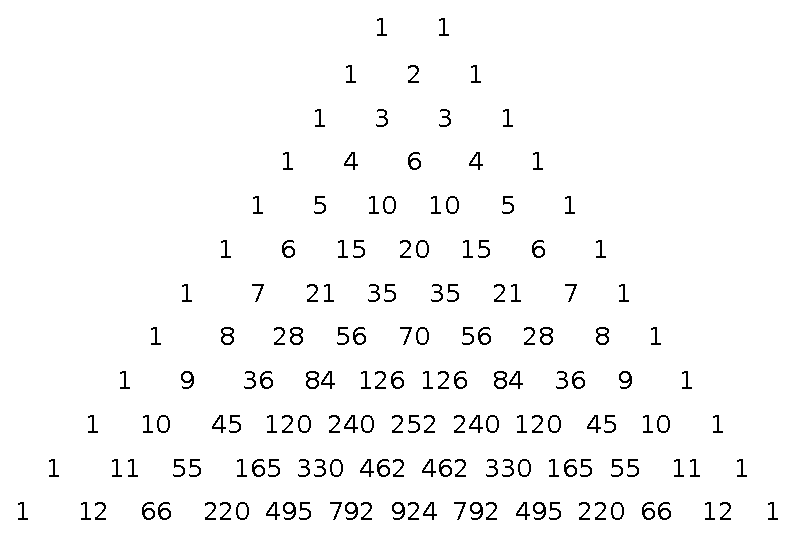
\includegraphics[scale=.8]{figure/fig1.eps}
\caption{}\label{fig01}
\end{figure}

rows from the top we have to book at row number $\alpha$ and row number $n-\alpha$ only, consider suitable products and take their maximum.

For $n=6$, $d=3$ we obtain $\tau = 10$, $\tau = 12$, $\tau_{3} = 9$ and $\tau = 12$. In the other hand $???$ can go upti $^6C_{3} = 20$ giving us several genuinely entangled vectors. It is clear how to proceed in general cases.
\end{example}
\end{proof}

Above results and discussion give complete information in certain special cases with a little more effort. We record them in the Example below.

\begin{example}\label{example-2.2}
 Let $F$, $\xi$ etc. be as above. Indeed we follow the notation terminology and results above freely. 
 
 \begin{enumerate}[label=(\roman*)]
 \item $\xi$ is a product vector in the following two cases
 
   \begin{enumerate}[label=(\alph*)]
   \item $l=1$, i.e; $F(\bold{\x}) = \lambda\bold{\x}^{k}$ for some scalar $\lambda \neq 0$ and $k \subset \Gamma_{n}$.
	\item $m=1$ i.e; $F(\bold{\x}) = a + b\x_{j}$ for some $j$ with $1 \leq j \leq n$ and $(a , b) \in \vertchar[.08ex]{C}^{2}$ with $b \neq 0$.
   \end{enumerate}
   
 \item Let us consider $F$ with $t \geq 2$, $m \geq 2$ and $d =1$. We have the following.
 
 \begin{enumerate}[label=(\alph*)]
 \item $\xi$ is not a product vector because $d < m$. Indeed, $F(\bold{\x}_{S_{F}})$ is irreducible. Here we set $F(\bold{\x}_{S_{F}}) = F(\bold{\x})$ only.
 \item If $S_{F} = \Gamma_{n}$, i.e; $m=n$, then $??$ is genuinely entangled. This does happen when $n=2$.
 \item Consider the case when $n \neq 3$ and $S_{F} \neq \Gamma_{n}$ and any ????? cut $(E, E')$. Then $???$ is a product vector in this cut if and only if either $E \supset S_{F}$ or $E' \supset S_{F}$.
  \end{enumerate}
 
 \item We now consider the case $n=2 =d = m \leq t$. Then $F$ has the form $F(\bold{\x}) = a_{0} + a_{1} \x_{1} + a_{2} \x_{2} + a_{3}\x_{1} \x_{2}$ with $a_{3} \neq 0$, $(a_{0}, a_{1}, a_{2}) \neq (0,0,0)$.
 
 \begin{enumerate}[label=(\alph*)]
  \item If $t=3$, then $\xi$ is entangled (and therefore, genuinely entangled).
 \item If $t = 2$ then the situation gets divided in three forms for $F$, viz, $F(\bold{\x}) = a_{0} + a_{3}\x_{1} \x_{2}$ with $a_{0} \neq 0$, giving rise to an entangled $\xi$ and $F(\bold{\x}) = a_{1}\x_{1} + a_{3}\x_{1}\x_{2} = \x_{1}(a_{1} + a_{3}\x_{2})$ with $a_{1}\neq  0$ or $F(\bold{\x}) = a_{2} \x_{2} + a_{3}\x_{1}\x_{2} = (a_{2} + a_{3}\x_{1})\x_{2}$ with $a_{2}\neq 0$. both giving rise to product vectors.
 
 \item If $t =4$, then each one of $a_{0}, a_{1}, a_{2}, a_{3}$ is non-zero. $\xi$ is a product vector if and only if $a_{0}a_{3}= a_{1}a_{2}$.
   \end{enumerate}
 
 \item Let $t=2$. Then $F(\bold{\x}) = a \bold{\x}^{k} + b \bold{\x}^{L}$ for some non-zero scalars $a$ and $b$ and distinct subsets $K$ and $L$ of $\Gamma_{n}$. So $F(\bold{\x}) = \bold{\x}^{K \cap L} (a \bold{\x}^{K L} + b \bold{\x}^{L K})$ and $K \triangle L = (K  L) \cup  (L K) \neq \phi$. We write $q(\bold{\x}_{K \triangle L})$ for the second factor. Then $q$ is irreducible.
 
 \begin{enumerate}[label=(\alph*)]
 \item $\xi$ is a product vector if and only if $\# K \triangle = 1$, i.e; either $K \subset L$ or $L \subset K$ and correspondingly $\#(L K) = 1$ or $\# (K L) = 1$.
 \item Given a bipartite cut $(E,E')$, $???$ is a product vector in this cut if and only if either $K \triangle L \subset E'$. This can happen only if $K \triangle ???$
 \item $\xi$ is genuinely entangled if and only if $K \cap L = \phi$ and $K \cup L = \Gamma_{n}$ i.e; $K \triangle L = \Gamma_{n}$ if and only if for $1 \leq j \leq n$, neither $\x_{j}$ is a factor of $F(\bold{\x})$ nor it is missing in $F(\bold{\x})$. 
 \end{enumerate}
 
 \item Let $t$ be any add prime.
 
 \begin{enumerate}[label=(\alph*)]
 \item $\xi$ is entangled because $t$ is not of the form $2^{u}$ for any non-negative integer $u$.
 \item $F(\bold{\x}) = \sum_{j=1}^{F} a_{j}\bold{\x}^{K_{j}}$ for some non-zero scalars $a_{j}$'s and distinct subsets $K_{j}$ of $\Gamma_{n}$. Let $K =\bigcap\limits_{j=1}^{t} K_{j}$, $L_{j} = K_{j} . ????$ for $1 \leq j \leq t$, $L =\bigcup\limits_{j=1}^{t}L_{j}$. Then $S_{F} = K \cup L = \bigcup\limits_{j=1}^{t} K _{j}$. Further $F(\bold{\x}) = \bold{\x}^{K}(\sum_{j=1}^{t} a_{j}\bold{\x}^{L_{j}})$. We write $q(\bold{\x}_{L})$ for the second factor. Then $q$ is irreducible because $t$ is prime and no $\x_{j}$ is a factor of $q(\bold{\x}_{L})$. Moreover, $S_{q} = L$ and $\# L \geq 2$.
 \item Give a biportite  and $(E, E')$, ??? product vector in this cut if and only ??? either $L \subset E$ or $L \subset E'$. This can happen only if $L ????$.
 \item $\xi$ is ???? entangled if and only if $K = \phi$ and $L = \Gamma_{n}$, i.e; $\bigcap\limits_{j=1}^{t} K, = \phi$ and $\bigcup\limits_{j=1}^{t} K = \Gamma_{n}$ of and nor $\x_{j}$ is missing in $F(\bold{\x})$.
  \end{enumerate}
 
 \end{enumerate}
 This ????? study to cases that ??? $n > 3$, $m \geq 2$, $d \geq 2$ and $???$ a composite number.
\end{example} 

\section{Polynomial Representation of Resonance Valence Bond States (RVB) and Their Quantum Entangement}\label{section-3}

For the sake of self-complateness and convenient notation and terminology we begin with the simple case of a singled a dimer and go upto that of ??? resonance ??? bond states with variable co-efficients. With the right choice made in Section~\ref{section-2} above, their polynomial representation turns ??? to be a homogeneous polynomial of small degree. This ??? the study of their quantum entanglement which requies new conditions that we introduce. For ???? we may refer to [1 to  12] or any other standard source.

\subsection{Basic definition and ????}\label{subsection-3.1}

Let $V \in \mathbb{N}$ and $n=2V$. We divide $\Gamma_{n} = \left\{j \in N : 1 \leq j \leq n\right\}$ into two equal parts $A$ and $B$, say $A = \left\{2^{t-1} : l \leq t \leq V\right\}$ and $B = \left\{ 2t : 1 \leq t \leq V \right\}$. For ?????? representations of various concepts we will mark points of $A$ by $\bullet$ and those of $B$ by $\odot$ and arrange them in different ways. For instance,

\begin{figure}
\centering
\includegraphics[scale=.8]{figure/fig2.eps}
\caption{}\label{fig02}
\end{figure}

is useful in the nearest neighbour (NN) context.

\begin{subsubsec}\label{subsubsection-3.1.1}
Coverings A bijective map $\Psi$ of $A$ to $B$ is called a covering, say $C$, of $\Gamma_{n}$. It can be given in terms of a permutation $\widetilde{\Psi}$ of $\Gamma_{n}$ by setting $\Psi(2t-1) = 2\widetilde{\Psi}(t)$ for $t \in \Gamma_{v}$.
  \begin{enumerate}[label=(\alph*)]
  \item $\Psi$ is called a nearest neighbour covering (???) $(NN)$ if $2(t-1) \leq \Psi(2t-1) \leq 2(t+1)$, i.e; $t-1 \leq \widetilde{\Psi}(t) \leq t H$(???) for $t \in \Gamma_{v}$. In other words, the permutation matrix of $\widetilde{\Psi}$ is handed matrix with band-width $\leq 1$.
   \item Samson and Ezermann [SE] study banded matrices and note in Remark 2.3 [SE] that the number of such matrices with bandwidth $\leq 1$ is the Fibonacci number $F_{v}$ with initial conditions $F_{1}=1 =F_{0}$.
   \item $\Psi$ is called a periodic $NN$ covering of we permit $\Psi(2v-1)$ to be 2 and $\Psi(1)$ to be 2v as well. In other words, we work in $\mathbb{Z} \md 2v$ .
   \item The number of all covering of $\Gamma_{n}$ is $\d{v}|$, the number of permutations of $\Gamma_{v}$.
    \item We will be considering various set $\underline{\overline\Psi}$ of covering with $\#\underline{\overline\Psi} \geq 2$ and $v \geq 2$. For $v=2$, $\#\underline{\overline\Psi}$ can only be 2, since the covering are only.
    
    \newpage
    
    \item Here are pictures of some easy coverings.
    
    \begin{figure}[h]
\centering
\includegraphics[scale=.8]{figure/fig3.1.eps}
\caption{}\label{fig03}
\end{figure}

  \end{enumerate}
\end{subsubsec}

%%%%%%%%%%%%%%%%%%%%%%%%%%%%%%%%21 page %%%%%%%%%%%%%%%%%%%%%%%%%%%%%%%%%%%%%%%%%%%%%%%%%%%%%%%%%%%%%%%%%%%%%
\begin{subsubsec}\label{subsubsection-3.1.2}

{\bfseries Resonance valence bond (RVB) states and Vectors.}

For $a\in A$, $b \in B$, we write $H_{a,b}$ for $\mathcal{H}_{a} \bigotimes \mathcal{H}_{b}$. We follow the polynomial representation as set out in section~\ref{section-2} above.

\begin{enumerate}[label=(\alph*)]
\item A dimer or a singlet at a, b is the unit vector
$$
[a, b] = \frac{1}{\sqrt{2}} (| \uparrow \rangle_{a} \otimes | \downarrow \rangle_{b}) = \frac{1}{\sqrt{2}}(| 0\rangle_{a} \otimes | \shortmid \rangle - | \shortmid \rangle_{a} \otimes | 0 \rangle_{b})\quad {\rm in} \quad  \mathcal{H}_{a,b} 
$$

Its polynomial representation is given by
\begin{equation*}
F_{a_{1}b}(\x_{a}, \x_{b}) = \frac{1}{\sqrt{2}}(\x_{b}- \x_{a})\tag{3.3}
\end{equation*}

\item Let  $C$ be a covering of $\Gamma_{n}$ i.e; a bijective map $\Psi$ of $A$ to $B$. We let $| C \rangle = | \Psi \rangle$ be the vector in $\mathcal{H}$ identified with $\bigotimes\limits_{a \in A} \quad \mathcal{H}_{a}\Psi_{(a)}$ given by $\bigotimes\limits_{a \in A} [a, \Psi(a)]$, i.e;,
\begin{gather*}
2^{-v/2} \bigotimes\limits_{a \in A} \left(| \uparrow \rangle_{a} \otimes | \downarrow \rangle_{\Psi (a)}) - | \downarrow \rangle_{a} \otimes | \uparrow \rangle_{\Psi (a)}\right)\\
= 2^{-v/2} \bigotimes\limits_{a\in A} \left(|0\rangle_{a} \otimes | 1 \rangle_{\Psi(a)} - |1 \rangle_{a} \otimes | 0 \rangle_{\Psi(a)}\right)
\end{gather*}
 
 
It is a unit vector and its polynomial representation is 
\begin{equation}
F_{\underline{\overline{\Psi}}} = 2^{-v/2} \prod\limits_{a\in A}(\x_{\Psi(a)}- \x_{a})\tag{3.4}\label{eq-3.4}
\end{equation}

It is a non-zero homogeneous polynomial of degree $d=v$ and its support is $S_{F_{\underline{\overline{\Psi}}}} = \Gamma_{n}$, i.e., $m=n$.

Indeed, 
\begin{align*}
F_{\Psi}(\bold{\x}) &= 2^{-v/2} \sum_{A_{1} \subset A}(-1)^{??? A_{1}} \bold{\x}^{A_{1}} \bold{\x}^{B\smallsetminus\Psi(A_{1})}\nonumber\\
& = 2^{-v/2} \sum_{\substack{A_{1} \subset A \\ \#A_{1} \leq v/2 \\ | \in A_{1}={\rm nu}/2 }} \left(\bold{\x}^{A_{1}} \bold{\x}^{B\smallsetminus \Psi (A_{1}) } + (-1)^{v} \bold{\x}^{A \smallsetminus A_{1}} \bold{\x}^{\Psi (A_{1})} \right)\tag{3.5}  
\end{align*}

Clearly, the number $t$ of terms in $F_{\Psi}$ is $2^{v}$ and $\bold{\x}^{k}$ is not a factor of $F_{\Psi}(\bold{\x})$ for any $\phi \neq K_{\neq} \subset \Gamma_{n}$.

\item Let $v \geq 2$ and $\underline{\overline{\Psi}}$ a set of coverings of $\Gamma_{n}$ with $s= \# \underline{\overline{\Psi}} \geq 2$. Then we write $| \underline{\overline{\Psi}}\rangle$ for the RVB vector $\frac{1}{\# \underline{\overline{\Psi}}} \sum_{\Psi \in \underline{\overline{\Psi}}} | \Psi \rangle$ in $\mathcal{H}$. We note that $|| \underline{\overline{\Psi}} || \leq |$ and we will come to its normalization later in (3.1.4).

\item The polynomial representation of $| \underline{\overline{\Psi}}\rangle$ is given by
\begin{equation}
F_{\underline{\overline{\Psi}}} = \frac{1}{\# \underline{\overline{\Psi}}} \sum_{\Psi \in \underline{\overline{\Psi}}} F_{\Psi} = \frac{1}{\# \underline{\overline{\Psi}}} \sum_{\substack{{A_{1} \subset A}\\ B_{1}\subset, \# B_{1}= \# A_{1}}} (-1)^{\# A_{1}} \# \left\{ \Psi \in \underline{\overline{\Psi}} : \Psi (A_{1}) = B_{1}\right\} \bold{\x}^{A_{1}} \bold{\x}^{B\smallsetminus B_{1}}\tag{3.6}\label{eq-3.6}
\end{equation}

Then $| \underline{\overline{\psi}} \rangle \neq 0$ simply because $0 \neq 2^{-v/2}(\bold{\x}^{B} + (-1)^{v} \bold{\x}^{A})$ is a part of $F_{\underline{\overline{\Psi}}}(\bold{\x})$.

Indeed, this also gives that $S_{F_{\underline{\overline{\Psi}}}} = \Gamma_{n}$, i.e., $m=n$ and $\bold{\x}^{K}$ is not a factor of $F_{\underline{\overline{\Psi}}} (\bold{\x})$ for any $\phi \neq K \subset \Gamma_{n}$.

\item Let $v \geq 2 $, $\underline{\overline{\Psi}}_{NN} =$ the set of nearest neighbour $(NN)$ coverings of $\Gamma_{n}$ and $\underline{\overline{\Psi}}_{PNN} =$ the set of periodic nearest neighbour $(PNN)$  covering of $\Gamma_{n}$. Then $|\underline{\overline{\Psi}}_{NN} \rangle$ and $| \underline{\overline{\Psi}}_{PNN} \rangle$ will be called the NN-RVB and the PNN-RVB vectors (in the context of n-qubit system).

We record some immediate applications of Theorem~\ref{thm-2.1}, 2.2 above is section~\ref{section-2} labelled as Theorem~\ref{thm-3.1} and Example~\ref{example-3.1}.

\end{enumerate}

\end{subsubsec}

\begin{thm}\label{thm-3.1}

We consider the vectors given in~\eqref{subsubsection-3.1.2} above in their respective spaces.

\begin{enumerate}[label=(\roman*)]

\item A dimer $[a, b]$, $| \Psi \rangle$, $| \underline{\overline{\Psi}} \rangle$ are all entangled.

\item Let $v \geq 2$ and $(E, E')$ a  bipartite cut of $\Gamma_{n}$.

   \begin{enumerate}[label=(\alph*)]
    \item $| \Psi \rangle$ is a product vector in the cut $(E, E')$ if and only if 
			\begin{align*}
			\Psi(E \cap A) &= E \cap B \quad \text{if and only if}\\
			\Psi(E' \cap A) &= E'\cap B \tag{3.7}\label{eq-3.7}
			\end{align*}
			
	 In this case we have $\# E$ and $\# E'$ are both even.
	 \item If $| \underline{\overline{\Psi}} \rangle$ is a product vector in the cut $(E, E')$, then 
	 		\begin{equation}
	 		 \Psi(E \cap A) = E \cap B \quad ({\text {equivalently}}, \Psi (E' \cap A) = E' \cap B)\; \text{for each}\; \Psi \;\text{in}\; \underline{\overline{\Psi}}\tag{3.8}\label{eq-3.8}   
	 		\end{equation}
	 		
	 	In this case, $\# E$ and $\# E'$ are both even.	
    \end{enumerate}
    
   \item For $v=2$, $| \underline{\overline{\Psi}} \rangle$ is genuinely entangled.
   
   \item For $\underline{\overline{\Psi}} $ NN or PNN, $|\underline{\overline{\Psi}}\rangle$ is genuinely entangled.
   
   \item (a) The converse of (ii) (b) holds for $v=3$ but not in general.
   
   (b) The converse of (ii) (b) holds for all $v \geq 3$ if we consider special cuts with $\min \left\{ \# E, \# E' \right\} = 2$.
\end{enumerate}
\end{thm}

\begin{proof}
\begin{enumerate}[label=(\roman*)]
 
 \item  It follows from Theorem~\ref{thm-2.1} (i) (a) because $d=v < 2 v =n$ for the corresponding polynomials. 

\item (a) The second equivalence is trivial. For the first one, the `if' part is immediate. For the  `only if' part, let, $p(\bold{\x}_{E}), q (\bold{\x}_{E'})$ be polynomials that satisfy $F(\bold{\x}) = p(\bold{\x}_{E}) q(\bold{\x}_{E'})$. Then by Theorem~\ref{thm-2.1} (iv) (b), $p(\bold{\x}_{E})$ and $q(\bold{\x}_{E'})$ are both homogeneous, say, of degree $v_{1}$ and $v_{2}$ respectively with $v_{1} \geq 1$, $v_{2} \geq 1$, $v_{1} + v_{2} = v$, $S_{p} =E$ and $S_{q} = E'$.  low by~\eqref{subsubsection-3.1.2} (b) $\bold{\x}^{A}$ and $\bold{\x}^{B}$ both occur in $F_{\Psi}(\bold{\x})$. The one and only one way it can happen is the $\bold{\x}^{E \cap A}$, $\bold{\x}^{E \cap B}$ occur in $p(\bold{\x}_{E})$, and $\bold{\x}^{E' \cap A}$ and $\bold{\x}^{E' \cap B}$ occur in $q(\bold{\x}_{E'})$. This gives that $\# E \cap A = \# E \cap B = v_{1}$ and $\# E' \cap A = \# E' \cap B =v_{2}$. Now $\bold{\x}^{E \cap A}$ $\bold{\x}^{E' \cap B}$ occurs in But this can happen for $F_{\Psi} (\bold{\x})$ if and only of $B \Psi(E \cap A) = E' \cap B$, i.e., $\Psi(E \cap A) = E \cap B$. As a consequence $\Psi (E' \cap A) = E' \cap B$ as well. This confirms the assertion already made about the relationships amongst cardinalties of the sets, $v_{1}$, $v_{2}$. Clearly $\# E = \# (E \cap A) + \# (E \cap B) = 2 v_{1}$.

(b) As noted in ~\ref{subsubsection-3.1.2} (c), $\bold{\x}^{A}$ and $\bold{\x}^{B}$ both occur in $F_{\overline{\Psi}}(\bold{\x})$. So arguments in the proof of part (ii) (a) above by replacing $F_{\Psi}$ by $F_{\underline{\overline{\Psi}}}$ with the addition of ``for some $\Psi \in \underline{\overline{\Psi}}$ in the sentence beginning with `But'. Now consider any $\varphi \in \underline{\overline{\x}}$. Then $\bold{\x}^{E \cap A} \bold{\x}^{B \smallsetminus \varphi (E \cap A)}$ occurs in $F_{\underline{\overline{\Psi}}}(\bold{\x})$ and, therefore, in $p(\bold{\x}_{E}) q(\bold{\x}_{E'})$. The only way this can happen is that $B \smallsetminus \varphi (E \cap A) = E' \cap B$, which gives, in turn, $\varphi(E \cap A) - E \cap B$. This completes the proof of the first assertion. The second statement following ?????.

\item For $v=2$, the condition~\ref{eq-3.8}   in (ii) (b) is note satisfied for any $\phi \neq E \subset \lceil_{4}$ as in clear from ~\ref{subsubsection-3.1.2} (e) above. (iii) It follow $\langle \neq \#$ from (ii)(b) and (c).

\item In view of (iii), it is enough to consider the case $v \geq 3$. Let, if possible, the condition in (ii) (b) the case $v \geq 3$. Let if possible, the condition in (ii)(b) be satisfied for some $E$ with $\phi \neq E_{\neq} \subset \neq_{n}$ and $\underline{\overline{\Psi}}= \underline{\overline{\Psi}}_{NN}$.

Consider any $2s-1 \in E \cap A$ with $1 \leq s\ leq v$. If $s < v$, then there exist $\Psi_{1}, \Psi_{2} \in \underline{\overline{\Psi}}$ with $\Psi_{1} (2s-1) = 2(s + 1)$ and $\Phi_{2} (2s+1) = 2(s+ 1)$. So $s(s+ 1) \in E \cap B$, which in turn, gives that $2s+1 \in E \cap A$. On the other hand, if $s > 1$, then there exist $\Psi_{3}, \Psi_{4} \in \underline{\overline{\Psi}}$ satisfying $\Psi_{3}(2s-1)= 2(s-1)$ and $\Psi_{3}(2s-3) =2 (s-1)$. So $2(s-1) \in E \cap B$ which leads to $2s-3 \in E \cap A$. Repeating the arguments iteratively we arrive at the conclusion that $\left\{2t-1 : 1 \leq t \leq v \right\} \subset E \cap A$. But that is not so. Hence $\underline{\overline{\Psi}}_{NN}$ is note a product vector in any bi?????? cut and is therefore genuinely entangled.  

Now we come to $\underline{\overline{\Psi}}_{PNN}$. Because $\underline{\overline{\Psi}}_{PNN} \supset \underline{\overline{\Psi}}_{NN}$, it cannot satisfy (\ref{subsection-3.6}) in (ii)(b) for any $E$ with $\phi \neq E \subset_{\neq} \Gamma_{n}$. Hence $\underline{\overline{\Psi}}_{PNN}$ is genuinely entangled.

\item 
\begin{enumerate}[label=(\alph*)]
\item For any bipartite cut $(E, E')$ of $\lceil_{6}$ with $\#E$ and $\#E'$ both even,\break $\min\left\{\# E, \# E'\right\}=2$. Suppose $\#E'=2$. Then for any $\Psi \in \underline{\overline{\Psi}}$, $\Psi (E' \cap A) = E' \cap B$,say, $\Psi(a) = b$ where $E'\cap A = \{a\}$, $E'\cap B=\{b\}$. So $\x_{b} \smallsetminus \x_{a}$ is a factor of $F(\bold{\x})$. Similarly for the case of $\# E=2$. So $\lceil\underline{\Psi}\rangle$ is a product vector in the cut $(E, E')$ by Theorem~\ref{thm-2.1}(ii)(a).

We shall give an example in Example~\ref{example-3.1} below to show that the converse of (ii)(b) in Theorem here does not hold in general.

\item We can formulate the proof on the lines of that of (a) above.

\end{enumerate}

\end{enumerate}

\end{proof}


\begin{definition}\label{def-3.1}
(i) We call $\underline{\overline{\Psi}}$ $\boldsymbol{\text{decomposable Via} ~E}$ if it satisfies the condition~\ref{subsection-3.6} in Theorem~\ref{thm-3.1}(ii)(b) above, i.e; $\Psi(E\cap A) = E\cap B$ for $\Psi \in \underline{\overline{\Psi}}$. (ii) $\underline{\overline{\Psi}}$ will be called $\boldsymbol{\rm decomposable}$ if it is decomposable via $E$ for some bipartite cut $(E, E')$. 
\end{definition}

\begin{example}\label{example-3.1}
We consider~\ref{subsubsection-3.1.1} $(F)$ above and use Theorem~\ref{thm-3.1} above freely.
\end{example}

\begin{enumerate}
\item Let $v=3$ and $\underline{\overline{\Psi}}$ consist of the two converings given in Figures. Then $\underline{\overline{\Psi}}$ is not decomposable. So $\lceil\underline{\Psi}$ is genuinely entangled.

\item Let $v=4$ and $\underline{\overline{\Psi}}$ consist of the two coverings in Figure\ref{fig03}. Then $\underline{\overline{\Psi}}$ is decomposable with $E= \{3,4,5,6\}$ serving the desired purpose. However,$\lceil\underline{\overline{\cup}}\rangle$ is note a product vector in the bipartite cut $(E, E')$  as can be seen by computing $F_{\underline{\overline{\Psi}}}$. In fact,
\begin{equation*}
\begin{split}
F_{\underline{\overline{\Psi}}}(\bold{\x}) = &\left(\x_{2} \x_{8} + \x_{1}\x_{7} - \x_{1}\x_{2} -\x_{7}\x_{8}\right)\left(\x_{4}\x_{6} + \x_{3}\x_{5}- \x_{3}\x_{4} - \x_{5}\x_{6} \right)\\
&+ \left(\x_{2}\x_{8} + \x_{1}\x_{7} - \x_{1}\x_{8}-\x_{2}\x_{7}\right) \left(\x_{4} \x_{6} + \x_{3} \x_{5} - \x_{3}\x_{6}-\x_{4} \x_{5}\right).
\end{split}
\end{equation*}

This can note be factored as as $p(\bold{\x}_{E})~q(\bold{\x}_{E'})$ for any polynomials $p$ and $q$ more are apart from $E$ there is no other subset $G$ with $\phi \neq G \subset_{\neq} \lceil_{6}$ that satisfies the condition~\ref{subsection-3.6} of decomposability. This show that the converse of Theorem~\ref{thm-3.1}(ii)(b) does not hold in  general.
\end{enumerate}

\begin{subsubsec}\label{subsubsection-3.1.3}
${{\text{\bf Concepts and properties if}}~ \mathbf{\underline{\overline{\Psi}}}~ \text{\bf related to decomposability}}.$

Let $v\geq 3$ and $\# \underline{\overline{\Psi}} \geq 2$.

\begin{enumerate}[label=(\alph*)]

\item  Let $\varphi_{1} = \left\{A_{1} \subset A : \# \left\{\Psi (A_{1}) : \Psi \in \underline{\overline{\Psi}} \right\} \right\} =1$. For $A_{1} \in \varphi_{1}$ we write $B_{1}$ for $\Psi(A_{1})$ for any (and thus for all) $\Psi \in \underline{\overline{\Psi}}$. Then $\phi, A \in \varphi_{1}$ and $\varphi_{1}$ is an algebra of subsets of $A$. As a consequence, $B_{1} = \left\{B_{1}= \Psi(A_{1}) : A_{1} \in \varphi_{1} \right\}$ is an algebra of subsets of $B$. In particular, \# $\varphi_{1} \geq 3$ if and only if \# $B_{1} \geq 3$. In this case, let $\varphi_{1}$ mix be the subset of $\varphi_{1}\{\phi\}$ consisting of its minimal subsets.

\item Now suppose \# $\varphi_{1} \geq 3$ and consider any $A_{1} \in \varphi_{1}$ with $\phi \neq A_{1}\neq A$. We set $E = A_{1} \cup B_{1}$. Then \# $E \neq \Gamma_{n}$. Also $\Psi(E \cap A) = E \cap B$ for $\Psi \in \underline{\overline{\Psi}}$. In other words, $\underline{\overline{\Psi}}$ is decomposable via $E$. for $\Psi \in \underline{\overline{\Psi}}$. In other words, $\underline{\overline{\Psi}}$ is decomposable via $E$. Then $\phi \neq E \cap A \neq A$ and $E \cap A \in \varphi_{1}$. This in then, gives that \# $\varphi_{1} \geq 3$. 

\item Because \# $\underline{\overline{\Psi}} \geq 2$, there exist $\Psi_{1}, \Psi_{2} \in \underline{\overline{\Psi}}$, $a \in A$, $b_{1} \neq b_{2}$ in $B$ with $\Psi_{1}(a_{1}) = b_{1}$, $\Psi_{2}(a_{1}) = b_{2}$. So $\{a_{1}\} \in \varphi_{1}$. Hence $\varphi_{1} \neq P_{A}$. Can de??? $\varphi_{1}$ is an algebra of subsets of $A$ too.

\item Consider $a_{1}$ as in (c) above and $a_{2}\neq a_{1}$ in $A$. If $\left\{a_{1}, a_{2} \right\} \in \varphi_{1}$ then $\Psi_{1}\left\{a_{1}, a_{2} \right\} = \left\{b_{1},\Psi_{1} (a_{2})\right\}$ has to be $\Psi_{2}\left\{a_{1}, a_{2} \right\} = \left\{b_{2},\Psi_{2} (a_{2})\right\}$ so that $\Psi_{1}(a_{2}) = b_{2}$ and $\Psi_{2}(a_{2}) = b_{1}$ and, thus, $\left\{a_{2}\right\} \notin \varphi_{1}$. On the other hand, if $\left\{a_{2}\right\} \in \varphi_{1}$, then $\Psi_{1}\left\{a_{1}, a_{2}\right\} = \left\{b_{1}, \Psi_{1}(a_{2})\right\} = \left\{b_{1}, \Psi_{2}(a_{2})\right\} \neq \left\{b_{2}m \Psi_{2}(a_{2})\right\}$ and, thus $\left\{a_{1}, a_{2} \notin \varphi_{1}\right\}$. Hence\, at most one of $\left\{a_{2}\right\}$, $\left\{a_{1}, a_{2}\right\}$ is in $\varphi_{1}$.

\item Let $\varphi_{2} = \left\{A_{2} \subset A : \# \{\Psi (A_{2}) : \Psi \in \underline{\overline{\Psi}}\} \geq 2\right\}$. Then $\varphi_{1} \cap \varphi_{2} = \phi$, $\varphi_{1} \cup \varphi_{2} = P_{A}$ and for $A_{2} \in \varphi_{2}$, $A \smallsetminus A_{2} \in \varphi_{2}$. By (c) above $\{a_{1}\} \in \varphi_{2}$ and therefore, $A\smallsetminus \{a_{1}\}$ and $\{a_{1}, a_{2}\}$ Now by (d), for $a_{2}\in A\smallsetminus\{a_{1}\}$, at least one of $\{a_{2}\}$
and $\{a_{1}, a_{2}\}$ is in $\varphi_{2}$ and neither of them or their complements in $A$ equal $\{a_{1}\}$ or $A\smallsetminus\{a_{1}\}$ because $v\geq 3$. Hence $\# \varphi_{2}\geq 4$.

\item $\phi$ and $A$ are in $\varphi_{1}$ and therefore, not in $\varphi_{2}$. So for $A_{2} \in \varphi_{2}$ $v-1 \geq \#$ $A_{2}\geq 1$ and, therefore, $^{v}C_{\# A_{2}} \geq v$.

\item 
\begin{align*}
F_{\underline{\overline{\Psi}}}(\bold{\x}) &= 2^{-v/2} \sum_{A_{1} \in \varphi_{1}}(-1)  \bold{\x}^{A_{1}} \x^{B\smallsetminus B_{1}} + \\
   & 2^{-v/2} \frac{1}{\# \underline{\overline{\Psi}}} \sum_{A_{2} \in \varphi_{2}} (-1)^{\# A_{2}} ??? \left(\sum_{B_{2} \in B} \# \left\{\Psi \in \underline{\overline{\Psi}} : \Psi(A_{2}) - B_{2}\right\}\bold{\x}^{B\smallsetminus B_{2}}\right)\tag{3.9}
\end{align*}

\item Let $A_{2} \in \varphi_{2}$. We write, for $B_{2} \subset B$, $A_{2}, B_{2}$ for $\frac{1}{\#\underline{\overline{\Psi}}} \# \{\Psi \in \underline{\overline{\Psi}} : \Psi (A_{2}) = B_{2} \}$. which in $\geq 0$.

We note that $C_{A_{2}B_{2}} \neq 0$ if and only if $B_{2} \in \{ \Psi (A_{2}) : \Psi \in \underline{\overline{\Psi}}\}$ .

In Particular, $C_{A_{2}B_{2}} = 0$ for $\# A_{2} \neq \# B_{2}$. Moreover $\sum_{B_{2 \subset B}}$ $C_{A_{2}, B_{2}} =1$ so $^{v}C_{\# A_{2}} \geq \# \{B_{2} \subset B : C_{A_{2}, B_{2}} \neq 0 \} \geq 2$.

This, in turn, gives that $C_{A_{2}, B_{2}}>0$ for at last two distinct subsets $B_{2}$ of $B$. As a consequence, $C_{A_{2}, B_{2}} < 1$ for all $B_{2} \subset B$.

\item Let 
\begin{align*}
F^{1}_{\underline{\overline{\Psi}}}(\bold{\x})  &= 2^{-v/2} \sum_{A_{1} \in \varphi_{1}}(1)^{\# A_{1}} \bold{\x}^{A_{1}} \bold{\x}^{B\smallsetminus} B_{1}\\
F^{2}_{\underline{\overline{\Psi}}}(\bold{\x})  &= 2^{-v/2} \sum_{A_{2} \in \varphi_{2}} \sum_{B_{1} \subset B} C_{A_{2}, B_{2}}(-1)^{\# A_{2}} \bold{\x}^{A_{2}} \bold{\x}^{B\smallsetminus}B_{2}\tag{3.10}\label{eq-3.10}\\
\text{So}\quad\quad F_{\underline{\overline{\Psi}}} (\bold{\x}) &= F^{1}_{\underline{\overline{\Psi}}} (\bold{\x}) + F^{2}_{\underline{\overline{\Psi}}} (\bold{\x})
\end{align*}

Let $t$, $t^{(1)}$, $t^{(2)}$ be the number of terms in $F_{\underline{\overline{\Psi}}}(\underline{x})$, $F^{(1)}_{\underline{\overline{\Psi}}}(\underline{x})$ and $F^{(2)}_{\underline{\overline{\Psi}}}(\underline{x})$ respectively then $t^{(1)} = \# \varphi_{1}$.

Using (h), we have $\sum_{A_{2} \in \varphi_{2}} \quad ^{v}C_{\# A_{2}} \geq t^{(2)} \geq 2 \# \varphi_{2}$. But by (e), $\# \varphi_{2} \geq 4$  and therefore, $f^{(2)} \geq 8$. Hence 
\begin{align*}
2^ {v} + \sum_{A_{2} \in \varphi_{2}}(^{v}C_{\# A_{2}}-1) &= \# \varphi_{1} + \sum_{A_{2} \in \varphi_{2}} ^{v}C_{\# A_{2}} \geq t^{(1)} + t^{(2)} = t \geq \# \varphi_{1} + 2 \# \varphi_{2} = \#P_{A} + \# \varphi_{2}\\
& = 2^{v} + \# \varphi_{2} \geq 2^{v} + 4 \tag{3.11}  
\end{align*}

\item If $\{a\} \in \varphi_{1}$ for some $a\in A$, then by (b) above and Theorem~\ref{thm-3.1} (v)(b), $|\underline{\overline{\Psi} \rangle}$ is a product vector in the bipartite cut $(E, E')$ with $E= \{a\}$.

\item We confine out attention to the case that $\{a\} \notin \varphi_{1}$, $a\in A_{1}$. In that case, $\{a\} \in \varphi_{2}$ for $a\in A$. So $\# \varphi_{2} \geq 2v$ because $\{A \smallsetminus \{a\}, \{a\} : a \in A \}$ are all different sets in view $v \geq 3$. This refines the second part of (3.11) viz; 
\begin{equation*}
t \geq 2^{v} + \# \varphi_{2} \geq 2^{v} + 2 \Psi = 2(2^{v-1} + v)\tag{3.12} 
\end{equation*} 

\end{enumerate}

We record a few test of decomposability which are ????? in 3.1.3 (a)\& (b), (i) and (k) above.

\end{subsubsec}

\begin{thm}\label{3.2}
{\bf (Tests of decomposability)}. Let $v\geq 3$ and $\# \underline{\overline{\Psi}} 2$.
\begin{enumerate}[label=(\roman*)]
\item The following are equivalent
\begin{enumerate}[label=(\alph*)]
\item $\underline{\overline{\Psi}}$ is decomposable.

\item $\# \varphi_{1} \geq 3$

\item $\# \varphi_{1} \geq 4$

\item The number $s$ of terms in $F_{\underline{\overline{\Psi}}}(\bold{\x})$ with $|$co-efficient$|= 2^{-v/2}$ is $\geq 3$.

\item The number $s$  as in (d) above is $\geq 4$.

\end{enumerate}

\item If $t < 2^{v} + 2v$ then $\underline{\overline{\Psi}}$ is decomposable via  some $a \in A$. Further in this case $| \underline{\overline{\Psi}} \rangle$ is a product vector in the bipartite cut $(E, E')$.
\end{enumerate}

\end{thm}

\begin{subsubsec}\label{subsubsection-3.1.4}
{\bf Normarization of $| \underline{\overline{\Psi}} \rangle$}. Let $v \geq 2$ and $\# \underline{\overline{\Psi}} \geq 2 $. (a) By \ref{subsubsection-3.1.1} (e) for $v=2$, there is only one $\underline{\overline{\Psi}}$. 

The polynomial representation of $| \underline{\overline{\Psi}} \rangle$ is given by
\begin{align*}
F_{\underline{\overline{\Psi}}} (\bold{\x}) &= \frac{1}{z^{2}}\left((\x_{2} - \x_{1}) (\x_{4} - \x_{3}) + (\x_{4}-\x_{1}) (\x_{2}-\x_{3})\right)\\
 &= \frac{}1{4} \left(2(\x_{1} \x_{3} + \x_{2} \x_{4}) - \x_{1} \x_{4}- \x_{2}\x_{3} -\x_{1}\x_{2}-\x_{3}\x_{4}\right)\\
\text{So} \quad || | \underline{\overline{\Psi}} \rangle || &= \frac{1}{4} \sqrt{\left(4+4+1+1+1+1\right)} = \frac{\sqrt{3}}{2}\tag{3.13}
\end{align*}

Hence the corresponding RVB state is $| \underline{\overline{\Psi}} \rangle  = \frac{2\sqrt{3}}{3} | \underline{\overline{\Psi}} \rangle$ and its polynomial representation is given by 
\begin{equation*}
F_{\underline{\overline{\Psi}}}(\bold{\x}) = \frac{\sqrt{3}}{6} \left(2(\x_{1}\x_{3} + \x_{2}\x_{4}) - \x_{1}\x_{4} - \x_{2}\x_{3}- \x_{1}\x_{4} -\x_{3}\x_{4}\right)\tag{3.14}
\end{equation*}

Let $v\geq 3$. We use\ref{subsubsection-3.1.3}(i). The terms of the polynomial representation of $F_{\underline{\overline{\Psi}}}(\bold{\x})$ coming from non-zero values of $C_{A_{2}, B_{2}}$'s are mutually orthogonal in $\lfloor^{2}\left(\prod^{n}\right)$, So
\begin{equation*}
|| | \underline{\overline{\Psi}} \rangle || = ||F_{\underline{\overline{\Psi}}}(\bold{\x})||_{2} = 2^{-v/2}\sqrt{\left(\# \varphi_{1}  + \sum_{A_{2} \in \varphi_{2}} \left(\sum_{B_{2} \subset B} C_{A_{2}, B_{2}}^{2}\right) \right)}\tag{3.15}
\end{equation*}

But for each $A_{2} \in \varphi_{2}$, $\# \{B_{2} \subset B  : C_{A_{2}, B_{2}} \neq 0\} \geq 2$ and $\sum C_{A_{2}, B_{2}} = 1$; by \ref{subsubsection-3.1.3} (h). So $\sum_{B_{2} \in B} C_{A_{2}, B_{2}} < 1$ for $A_{2} \in \varphi_{2}$.

Hence
\begin{equation*}
|| | \underline{\overline{\Psi}} \rangle || < 2^{-v/2} (\# \varphi_{1} + \# \varphi_{2}) =1\tag{3.16}
\end{equation*}

The corresponding RVB state, say $\widetilde{| \underline{\overline{\Psi}} \rangle} = \frac{1}{|| | \underline{\overline{\Psi}} \rangle||} | \underline{\overline{\Psi}} \rangle$ and its polynomial representation is 
\begin{equation*}
\widetilde{F}_{\underline{\overline{\Psi}}} (\bold{\x}) = \frac{1}{|| | \underline{\overline{\Psi}} \rangle||} F_{\underline{\overline{\Psi}}}(\bold{\x})\tag{3.17}
\end{equation*}

\end{subsubsec}

\begin{subsubsec}\label{subsubsection-3.1.5}
{\bf Motivation for factor ability of sets of coverings}. Theorem~\ref{thm-3.1} and \ref{subsubsection-3.1.3} permit us to confine out attention to $v\geq 3$ and decomposable coverings $\underline{\overline{\Psi}}$ with $\# \underline{\overline{\Psi}} \geq 2$ and $\{a\} \notin \varphi_{1}$, for any $a \in A$ on the one hand and motivate the new concept of factorability of $\underline{\overline{\Psi}}$ on the other hand.

%%%%%%%%%%%%%%%%%%%%%%%%%%%%%%%%%31%%%%%%%%%%%%%%%%
\begin{enumerate}[label=(\alph*)]
\item Suppose $\underline{\overline{\Psi}}$ is decomposable via $E$. Let $v_{1}= \# E \cap A$, $v_{2} = \# E' \cap A$

Let $\overline{\bold{\Psi}}_{E} = \left\{ \Psi /E : \Psi \in \overline{\bold{\Psi}}\right\}$ and $\overline{\bold{\Psi}_{E'}} = \left\{\Psi/E^{-1}: \Psi \in \overline{\bold{\Psi}}\right\}$.

We may set up label things $\left\{\Psi_{\alpha}^{E} : 1 \leq j \leq j^{1} \right\}$ and $\left\{\Psi_{k}^{E'} : 1 \leq k \leq k'\right\}$ for $\overline{\bold{\Psi}}_{E}$ and $\overline{\bold{\Psi}}_{E'}$ respectively. Then $\max\left\{j^{-1}, k'\right\} \geq 2$ simply because $\# \overline{\bold{\Psi}} \geq 2$. 

\item For any bijective  maps $\Psi_{1} : E \cap A \longrightarrow E \cap B$ and $\Psi_{2} : E' \cap A \longrightarrow E' \cap B$

We write $\Psi_{1} \times \Psi_{2}$ for the bijective map of $A$ to $B$ given by
\[
(\Psi_{1} \times \Psi_{2})~(a) =  
\begin{cases*}
\Psi_{1}(a),~~ \text{if}~~ a\in E\tag{3.18} \\
\Psi_{1}(a),~~ \text{if}~~a \in E' 
\end{cases*}
\]

For instance, $\Psi \in \overline{\bold{\Psi}}$ can be written as $\Psi_{E} \times \Psi_{E'}$.

\item Let $\overline{\bold\Phi}_{1}$ and $\overline{\bold{\Phi}}_{2}$ be any two sets of bijective maps $\varphi_{1}$ and $\varphi_{2}$ of in $E \cap A$ to $E \cap B$ and on $E' \cap A \rightarrow E' \cap B$  respectively. These we denote $\{ \varphi_{1} \times \varphi_{2} : \varphi \in \overline{\bold\Phi}_{1}, \varphi_{2} \in \overline{\bold\Phi}_{2}\}$ by $\overline{\bold\Phi}_{1} \times \overline{\bold\Phi}_{2}$.

\item For the sake of conveniende, we call $\psi_{1}$ and $\psi_{2}$ as in (b) \textbf{converings of $\mathbf{E}$ and $\mathbf{E'}$} respectively. We note 
that

 \begin{equation}
 \overline{\bold{\psi}}=????_{\Psi \in \overline{\bold\Psi}} \left(\{\psi/E\} \times \{\psi/E' \} \right) \quad \overline{\bold\psi}_{E} \times \overline{\bold\psi}_{E'} = \left\{\psi_{j}^{E} \times \psi_{R}^{E'} : 1 \leq j \leq j', 1 \leq k \leq k'\right\}\tag{3.19}\label{eq-3.19}
 %~ \overline{\bold{\psi}} = ????_{\Psi \in \overline{\bold\Psi}}} \left(\{\psi/E\} \times \{\psi/E' \} \right)
 %~ \quad \overline{\bold\psi}_{E} \times \overline{\bold\psi}_{E'} = \left\{\psi_{j}^{E} \times \psi_{R}^{E'} : 1 \leq j \leq j', 1 \leq k \leq k'\right\}
\end{equation}


\item We may picuture $\overline{\bold\psi}_{E} \times \overline{\bold\psi}_{E'}$ as a rectangular array $\varphi$ of dots, or, for that matter the $k' \times j'$ matrix $M$ with all entries 1. The $\overline{\bold\Psi}$ is a subset of $R$. haring at least on dot in each row and at least one dot in each column. The corresponding matrix for $\overline{\boldsymbol{\psi}}$ is a matrix of 0's or 1's with sum of each row and sum of. 
\end{enumerate}
\end{subsubsec}

\begin{definition}\label{definition-3.2}
Let $v \geq 3$ and $\overline{\boldsymbol{\psi}}$ a set of coverings of $\Gamma_{n}$ with $\# \overline{\boldsymbol{\psi}} \geq 2$. Let $(E, E')$ be a bipartite cut. We define cartiain types for $\overline{\boldsymbol{\psi}}$. 
\end{definition}

\begin{enumerate}[label=(\roman*)]

\item $\overline{\boldsymbol{\psi}}$ is \textbf{factorable via $\mathbf{E}$} if for some $\overline{\boldsymbol{\phi}}_{1}$ and $\overline{\boldsymbol{\phi}}_{2}$ of coverings of $E$ and $E'$ respectively, $\overline{\boldsymbol{\psi}} = \overline{\boldsymbol{\phi}}_{1} \times \overline{\boldsymbol{\phi}}_{2}$. In this case $\overline{\boldsymbol{\psi}}$ is decomposable vai $E$, $\overline{\boldsymbol{\phi}}_{1}= \overline{\boldsymbol\psi}_{E}$, $\overline{\boldsymbol{\phi}}_{2}= \overline{\boldsymbol\psi}_{E'}$, so that $\overline{\boldsymbol\psi}= \overline{\boldsymbol\psi}_{E} \times \overline{\boldsymbol\psi}_{E'}$ and $\# \overline{\psi}~~\# \overline{\boldsymbol\psi}_{E} \cdot \# \overline{\boldsymbol\psi}_{E'}$. These are indeed equivalent conditions in place of factorability and we may use the names \textbf{a grid of full-size} as well.

\item Let $\overline{\boldsymbol{\psi}}$ be decomposable via $E$. We say that $\overline{\boldsymbol{\psi}}$ is \textbf{flat} or \textbf{a pole} vai $E$  accordings  as $\# \overline{\boldsymbol{\psi}}_{E'} =1$ or $\overline{\boldsymbol{\psi}}_{E}=1$ respectively. In both these cases, $\overline{\boldsymbol{\psi}} = \overline{\boldsymbol{\psi}}_{E} \times \overline{\boldsymbol{\psi}}_{E'}$ so that $\overline{\boldsymbol{\psi}}$ is factorable. This does happen if $\#E'=2$ or $\# E=2$ respectively.

\item $\overline{\boldsymbol{\psi}}$ is \textbf{sleep} or \textbf{diazonal} via of $E$ of $\psi_{E}$'s are all distinct and $\psi_{E'}$'s are all distinct as $\psi$ varies in $\overline{\boldsymbol{\psi}}$, in other words, $j=k' = \# \overline{\boldsymbol{\psi}}$, or equivalently, $\psi \longrightarrow \psi/E$ and $\psi \longrightarrow \psi/E'$ are injective maps on $\overline{\boldsymbol{\psi}}$ to the sets of coverings of $E$ and $E'$ respectively.

\item $\overline{\boldsymbol{\psi}}$ is \textbf{hilly} via $E$ if $\overline{\boldsymbol{\psi}}$ is decomposable via $E$ but neither factorable nor sleep via $E$.

\item $\overline{\boldsymbol{\psi}}$ is \textbf{factorable} (flat, a pole) if it is \textbf{factorable} via $E$ for some $\phi \neq E \subset_{\#} \Gamma_{n}$.

\end{enumerate}

\begin{example}\label{example-3.2}
Following pictures serve as examples for the concepts defined above.

(a) 
\begin{figure}[h]
\centering
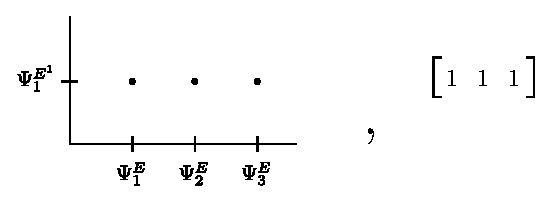
\includegraphics[scale=1.37]{figure/fig4.eps}
\caption{Flat}\label{fig04}
\end{figure}

\newpage
(b) 
\begin{figure}[h]
\centering
\includegraphics[scale=1.3]{figure/fig5.eps}
\caption{Pole}\label{fig05}
\end{figure}

(c)
\begin{figure}[h]
\centering
\includegraphics[scale=1.3]{figure/fig6.eps}
\caption{Grid, Factorable}\label{fig06}
\end{figure}

\newpage

(d)
\begin{figure}[h]
\centering
\includegraphics[scale=1.2]{figure/fig7.eps}
\caption{Steep}\label{fig07}
\end{figure}

(e)
\begin{figure}[h]
\centering
\includegraphics[scale=1]{figure/fig8.eps}
\caption{}\label{fig05}
\end{figure}

\end{example}

\begin{thm}\label{thm-3.3}
It $\overline{\boldsymbol{\psi}}$ is factorable via $E$ Then $| \overline{\boldsymbol{\psi}} \rangle$ is a product vector in the bipartite cut $(E, E')$. In particular, it is so if $\overline{\boldsymbol{\Psi}}$ is flat or a pole via $E$.
\end{thm}

\begin{proof}
It is is immediate from definition that 
\begin{equation}
| \overline{\boldsymbol{\psi}} = \frac{1}{\# \overline{\boldsymbol{\Psi}}} \sum_{\substack{1 \leq j \leq j'}\\ 1 \leq k \leq k'} | \psi^{E}_{j} \rangle \bigotimes | \psi_{k}^{E'} \rangle = \frac{1}{\# \overline{\boldsymbol{\Psi}}}\left(\sum_{j=1}^{j} | \psi_{j}^{E} \rangle\right) \bigotimes \left(\sum_{k=1}^{k'} | \psi_{k}^{E'}\right) \tag{3.20}\label{eq-3.20}
\end{equation}

Hence $| \overline{\boldsymbol{\Psi}}\rangle$ is a product vector in the cut $(E, E')$.

\end{proof}


\begin{subsubsec}\label{subsubsection-3.1.6}

\textbf{Entanglement properties of $\mathbf{| \overline{\boldsymbol{\psi}} \rangle}$ via polynomial representation.} In new of Theorems~\ref{thm-3.1}, \ref{thm-3.3} and intermediary discussion we can confine our attention to the case when $v \geq 4$, $\overline{\bold{\Psi}}$ is decomposable via some  $E$ with $\phi \neq E_{\#} \subset \Gamma_{n}$ and $\Phi~~ \overline{\boldsymbol{\Psi}}$ is not factorable. We will do a little representation here in connection with polynomial representation of $| \overline{\boldsymbol{\Psi}} \rangle$ to streamline the proof of our next Theorem. We will use the notation and terminology above, particularly the lot in \eqref{subsubsection-3.1.5} above.
\end{subsubsec}

\begin{enumerate}[label=(\alph*)]

\item The polynomial representation of the unit vectors $| \Phi_{1} \rangle$, $| \Phi_{2} \rangle$, $| \Phi_{1} \times \Phi_{2} \rangle$  in $\mathcal{H}_{E}$, $\mathcal{H}_{E'}$, $\mathcal{H}$ respectively are given by 
\begin{align*}
F_{\Psi_{1} \times \Psi_{2}} (\boldsymbol{\x}_{E}) & =  2^{-v_{1}/2} \prod_{a\in E \cap A}(\x_{\Psi_{1}(a)}- \x_{a}),~~\\
 &\qquad\qquad\quad F_{\Psi_{1} \times \Psi_{2}} (\boldsymbol{\x}_{E'})= 2^{-v_{2}/2} \prod_{a \in E' \cap A}(\x_{\Psi_{2}(a)}-\x_{a})\\
F_{\Psi_{1} \times \Psi_{2}} (\boldsymbol{\x}) &= 2^{-v/2} \prod_{a \in A} (\x_{\Psi_{1} \times \Psi_{2}(a)} - \x_{a})\\
F_{\Psi_{1} \times \Psi_{2}} (\boldsymbol{\x}) &= F_{\Psi_{1}} (\boldsymbol{\x}_{E})~~ F_{\Psi_{2}}(\boldsymbol{\x}_{E'})\tag{3.21}
\end{align*}

This justifies the rotation $\Psi_{1} \times \Psi_{2}$ set up in \ref{subsubsection-3.1.5} (b) above.

\item For $1 \leq j \leq j'$, let $T_{j} = \left\{k : 1 \leq k \leq k', \Psi_{j}^{E} \times \Psi_{k}^{E'} \in \overline{\boldsymbol{\Psi}}\right\}$, and for $1 \leq k \leq k'$, let $S_{E} = \left\{j : 1 \leq j \leq j', \Psi_{j}^{E} \times \Psi_{K}^{E'} \in  \overline{\boldsymbol{\Psi}}\right\}$. Then all these sets are non-empty  and $\overline{\boldsymbol{\Psi}} = \underset{j=1}{\overset{j'}{\bigcup}} ~~ \underset{R \in T_{j}}{\overset{}\bigcup} \left\{\Psi_{j}^{E} \times \Psi_{K}^{E'}\right\} = \underset{K=1}{\overset{k'}{\bigcup}}~~ \underset{j\in S_{k}}{\overset{}{\bigcup}}\left\{\Psi_{j}^{E} \times \Psi_{K}^{E'} \right\}$.

The unions are all disjoint and $s = \# \overline{\boldsymbol{\Psi}} = \underset{j=1}{\overset{j}{\sum}} \# T_{j} = \underset{k=1}{\overset{R'}{\sum}} \# S_{k}$.

We may express concepts in Definition~\ref{definition-3.2} in terms of $\# T_{j}$ , $\# S_{k}$ for $1 \leq k \leq k'$ For instance, $\overline{\boldsymbol{\Psi}}$ is factorable if and only if $\# T_{j} = k'$ for $1 \leq j \leq j'$ if and only if $\# S_{k} = j'$ for $1 \leq k \leq k'$ if and only $\therefore~ ??? = \# \overline{\boldsymbol{\Psi}} = j'^{k'}$.  

\item For $\Psi \in {\boldsymbol{\Psi}}$ let $p_{\Psi} ({\boldsymbol{\x}}_{E}) = p_{\boldsymbol{\x}_{E}}= 2^{v/2}F_{\Psi/E}({\boldsymbol{\x}}_{E})= \prod\limits_{\substack{a\in E \cap A}}(\x_{\Psi(a)}- \x_{a})$ and $q_{\Psi}({\boldsymbol{\x}}_{E'}) = q_{\Psi/E'}(\boldsymbol{\x}_{E}) = 2^{v_{2}/2} F_{\Psi/E'} ({\boldsymbol{\x}}_{E'}) = \prod\limits_{\substack{a \in E' \cap A}} (\x_{\Psi(a)} - \x_{a})$.

Set 
\begin{equation}
p^{0}_{\Psi}(\boldsymbol{\x}_{E}) = p^{0}_{\Psi/E}(\boldsymbol{\x}_{E}) = \sum_{\phi \neq A_{1_{\neq}} \subset E \cap A}(-1)^{\# A_{1}} {\boldsymbol{\x}^{A_{1}}} {\boldsymbol{\x}^{E \cap B \smallsetminus \Psi(A_{1})}}\tag{3.22}\label{eq-3.22}
\end{equation}
and 
\begin{equation}
q_{\Psi}^{0} (\boldsymbol{\x}_{E'}) = q^{0}_{\Psi/E'}(\boldsymbol{\x}_{E'})= \sum_{\phi \neq A_{2_{\neq}} \subset E' \cap A}(-1)^{\# A_{s}} {\boldsymbol{\x}^{A_{s}}} {\boldsymbol{\x}^{E' \cap B \smallsetminus \Psi(A_{2})}}\tag{3.23}\label{eq-3.23}
\end{equation}
Then
\begin{equation}
p_{\Psi}(\boldsymbol{\x}_{E}) = \boldsymbol{\x}^{E \cap B} + (-1)^{v_{1}} \boldsymbol{\x}^{E \cap A} + p^{0}_{\Psi}(\boldsymbol{\x}_{E})\tag{3.24}
\end{equation}
and
\begin{equation}
q_{\Psi}(\boldsymbol{\x}_{E'}) = \boldsymbol{\x}^{E' \cap B} + (-1)^{v_{2}} \boldsymbol{\x}^{E' \cap A} + q^{0}_{\Psi}(\boldsymbol{\x}_{E'})\tag{3.25}
\end{equation}

\item Let $s= \# \overline{\boldsymbol{\Psi}}$. We set $| \overline{\boldsymbol{\psi}} \rangle = 2^{v/2} \# \overline{\boldsymbol{\psi}} |\overline{\boldsymbol{\psi}} \rangle$. Its $p$ entanglement properties are same as that for $| \overline{\boldsymbol{\psi}} \rangle$.

Its polynomial representation has coefficients as integers and that is convenient to work with.

Indeed,
%~ \begin{equation}
\begin{align*}
F_{\overline{\boldsymbol{\Psi}}}(\boldsymbol{\x}) &= \sum_{\Psi \in \overline{\boldsymbol{\Psi}}} p_{\Psi} (\boldsymbol{\x}_{E})~~ q_{\Psi} (\boldsymbol{\x}_{E'})\\
&= \sum_{\Psi \in \overline{\boldsymbol{\Psi}}} \Bigg((\boldsymbol{\x}^{B}) + (-1)^{v}~~\boldsymbol{\x}^{A} + (-1)^{v_{1}}~~ \boldsymbol{\x}^{E \cap A} ~~\boldsymbol{\x}^{E'\cap B} + (-1)^{v_{2}}~~ \boldsymbol{\x}^{E \cap B}~~ \boldsymbol{\x}^{E' \cap A})\\ 
 &\quad  \left(\boldsymbol{\x}^{E \cap B} + (-1)^{v_{1}}~~ \boldsymbol{\x}^{E \cap A}\right)~~q_{\Psi}^{0} (\boldsymbol{\x}_{E'})  + p_{\Psi}^{0}(\boldsymbol{\x}_{E})~~ \left(\boldsymbol{\x}^{E' \cap B} + (-1)^{v_{2}}~~ \boldsymbol{\x}^{E' \cap A} \right)\\
 &\quad p_{\Psi}^{0}~~ (\boldsymbol{\x}_{E})~~ q_{\Psi}^{0}(\boldsymbol{\x}_{E'}) \Bigg)\\
 & = \# \overline{\boldsymbol{\Psi}} \left(\boldsymbol{\x}^{B} + (-1)^{v} \boldsymbol{\x}^{A} + (-1)^{v_{1}} \boldsymbol{\x}^{E \cap A} \boldsymbol{\x}^{E' \cap B} + (-1)^{v_{2}} \boldsymbol{\x}^{E \cap B} \boldsymbol{\x}^{E' \cap A} \right)\\
 &\quad + \left(\boldsymbol{\x}^{E \cap B} + (-1)^{v_{1}} \boldsymbol{\x}^{E \cap A}\right) \sum_{\Psi \in \overline{\boldsymbol{\Psi}}} q_{\Psi}^{0}(\boldsymbol{\x}_{E'}) + \sum_{\Psi \in \overline{\boldsymbol{\Psi}}} p_{\Psi}^{0}(\boldsymbol{\x}_{E}) \\
 &\hspace{7cm} \left(\boldsymbol{\x}^{E' \cap B} + (-1)^{v_{2}} \boldsymbol{\x}^{E \cap B} \boldsymbol{\x}^{E' \cap A} \right)\\
 & \quad + \sum_{\Psi \in \overline{\boldsymbol{\Psi}}} p_{\Psi}^{0} (\boldsymbol{\x}_{E}) q^{0}_{\Psi} (\boldsymbol{\x}_{E'})\tag{3.26}\label{eq-3.26}
\end{align*}
%~ \end{equation}

\item Consider homogeneous polynomials $p(\boldsymbol{\x}_{E})$ and $q(\boldsymbol{\x}_{E'})$ of degrees $v_{1}$ and $v_{2}$ respectively. They have the form
$p(\boldsymbol{\x}_{E}) = \delta \boldsymbol{\x}^{E \cap A} + \beta\boldsymbol{\x}^{E \cap B} + p_{0}(\boldsymbol{\x}_{E})$ with
\begin{equation}
p_{0}(\boldsymbol{\x_{E}}) = \sum\left\{\delta_{A_{1}, B_{1}} \boldsymbol{\x}^{A_{1}} \boldsymbol{\x}^{E \cap B \smallsetminus B_{1}} : \phi \neq A_{1 \neq} \subset E \cap A, \phi \neq B_{1 \neq} \subset E \cap B, \# A_{1}= \# B_{1}\right\}\tag{3.27}\label{eq-3.27} 
\end{equation}

and $q(\boldsymbol{\x}_{E'}) = \delta^{1} \boldsymbol{\x}^{E' \cap A} + \beta^{1} \boldsymbol{\x}^{E' \cap B} + q_{0}(\boldsymbol{\x}_{E'})$ with
\begin{equation}
q_{0}(\boldsymbol{\x}_{E'}) = \sum \left\{\delta'_{A_{1}, B_{2}} \boldsymbol{\x}^{A_{2}} \boldsymbol{\x}^{E' \cap B \smallsetminus B_{2}} : \phi \neq A_{2 \neq} \subset E' \cap A, \phi \neq B_{2 \neq} \subset E' \cap B, \# A_{2} = \# B_{2}\right\}\tag{3.28}
\end{equation}

where $\delta, \beta, \delta', \delta{'}, \beta_{'}, \delta_{A_{1}, B_{1}}$ are all scalars.

So
\begin{align*}
p(\boldsymbol{\x}_{E}) q (\boldsymbol{\x}_{E'}) &= \delta \delta' \boldsymbol{\x}^{A} + \beta \beta' \boldsymbol{\x}^{B} + \delta \beta' \boldsymbol{\x^{E \cap A}} \boldsymbol{\x}^{E' \cap B} + \delta'\beta \x^{E' \cap A} \boldsymbol{\x}^{E \cap B} +\\
&\quad(\alpha \boldsymbol{\x}^{E \cap A} + \beta \boldsymbol{\x}^{E \cap B}) q_{0}(\boldsymbol{\x}_{E'}) + p_{0}(\x_{E}) (\delta' \boldsymbol{\x}^{E' \cap A} +\beta' \boldsymbol{\x}^{E' \cap B}) +\\
&\quad p_{0}(\boldsymbol{\x}_{E}) q_{0}(\boldsymbol{\x}_{E'})\tag{3.29}
\end{align*}
 
\item We compare (3.26) in (d) and (3.29) in (e) above. 

We obtain that $\widetilde{F}_{\boldsymbol\Psi}(\boldsymbol{\x}) = p(\boldsymbol{\x}_{E}) q(\boldsymbol{\x}_{E'})$ if and only if
\begin{align*}
\beta \beta' &= s = (-1)^{v} \alpha \alpha' = (-1)^{v_{1}} \alpha \beta' = (-1)^{v_{2}} \alpha' \beta\tag{3.30}\label{eq-3.30}\\
\beta q_{0}(\boldsymbol{\x}_{E'}) &= \sum_{\psi \in \boldsymbol{\Psi}} q_{\Psi}^{0}(\boldsymbol{\x}_{E'}) = (-1)^{v_{1}} \alpha q_{0} (\boldsymbol{\x}_{E'})\tag{3.31}\label{eq-3.31}\\
\beta' p_{0}(\boldsymbol{\x}_{E}) &= \sum_{\psi \in \boldsymbol{\Psi}} p^{0}_{\psi} (\boldsymbol{\x}_{E}) = (-1)^{v_{2}} \delta' p_{0} (\boldsymbol{\x})\tag{3.32}\label{eq-3.32}\\
 \text{and}\quad p_{0}(\boldsymbol{\x}_{E}) q_{0}(\boldsymbol{\x}_{E'}) &= \sum_{\psi \in \boldsymbol{\Psi}} p^{0}_{\psi} (\boldsymbol{\x}_{E}) q^{0}_{\psi} (\boldsymbol{\x}_{E'}) \tag{3.33}\label{eq-3.33}
\end{align*}
 
 \item Let us first consider the case when this does happen By (3.30) $\alpha = (-1)^{v_{1}} \beta$, $\alpha' = (-1)^{v_{2}} \beta'$ and $\alpha, \beta, \alpha', \beta'$ are all non-zero.
 
 So we may take $\beta = s$, $\delta = (-1)^{v_{1}} s$, $\beta' = 1$, $\delta' = (-1)^{v_{2}}$ and multiply $p_{0}(\boldsymbol{\x}_{E})$ and $q_{0}(\boldsymbol{\x}_{E'})$ by suitable scalars if the need be and retain the same notation for them. Then~\eqref{eq-3.31} and \eqref{eq-3.32} give $s q_{0}(\boldsymbol{\x}_{E'}) = \sum\limits_{\psi \in \boldsymbol{\Psi}} q_{\psi}^{0} (\boldsymbol{\x}_{E'})$ and $p_{0}(\boldsymbol{\x}_{E}) = \sum\limits_{\psi \in \boldsymbol{\Psi}} p^{0}_{\psi}(\boldsymbol{\x}_{E})$. This turns~\eqref{eq-3.33} into
 \begin{equation}
 \left(\sum_{\psi \in \boldsymbol{\Psi}} p^{0}_{\psi}(\boldsymbol{\x}_{E})\right) \left(\sum_{\psi \in \boldsymbol{\Psi}} q^{0}_{\psi} (\boldsymbol{\x}_{E'})\right) = s \sum_{\psi \in \boldsymbol{\Psi}} p^{0}_{\psi} (\boldsymbol{\x}_{E}) q^{0}_{\psi}(\boldsymbol{\x}_{E'})\tag{3.34}\label{eq-3.34} 
  \end{equation}

For notational convenience, We write $p_{\psi^{E}}^{0} (\boldsymbol{\x}_{E})$ as $p^{0}_{j}(\boldsymbol{\x}_{E})$ and $q^{0}_{\psi_{k}^{E'}} (\boldsymbol{\x}_{E'})$ as $q_{k}^{0}(\boldsymbol{\x}_{E'})$ for $1\leq j \leq j'$, $1\leq k \leq k'$. 

We expand both sides of \eqref{eq-3.34} using (b) above in parts.

\begin{align*}
\text{L.H.S}~~\text{of}~~{\eqref{eq-3.34}} &= \left(\sum_{j=1}^{j'}  \# T_{j} p_{j}^{0}(\boldsymbol{\x}_{E})\right)\left(\sum_{R=1}^{k'} \#S_{k}~ q_{R}^{0}(\boldsymbol{\x}_{E'})\right)\\
&= \sum_{j=1}^{j'} \sum_{k=1}^{k'} \# T_{j} \#S_{k} p_{j}^{0}(\boldsymbol{\x}_{E}) q_{k}^{0}(\boldsymbol{\x}_{E'}).\tag{3.35}\label{eq-3.35}
\end{align*}

Now by (b) above $s= \sum_{k=1}^{k'} \# S_{k} = \sum_{j=1}^{j'} \# T_{j}$.

R.H.S of \eqref{eq-3.34}
\begin{equation}
s\sum_{j=1}^{j'} p_{j}^{0} (\boldsymbol{\x}_{E}) \left(\sum_{l \in T_{j}} q_{l}^{0}(\boldsymbol{\x}_{E'})\right) = s\sum_{k=1}^{k}  \left(\sum_{t \in S_{k}}  p_{T}^{0} (\boldsymbol{\x}_{E})\right) q_{R}^{0} (\boldsymbol{\x}_{E'})\tag{3.36}\label{eq-3.36}
\end{equation}

Equating L.H.S  and R.H.S of~\eqref{eq-3.34}, we obtain
\begin{equation}
\sum_{j=1}^{j'} p_{j}^{0}(\boldsymbol{\x}_{E}) \left(\sum_{l\in T_{j}} (\# T_{j} \# S_{l} -s) q_{l}^{0}(\boldsymbol{\x}_{E'}) + \sum_{\substack{1 \leq k \leq k' \\ k \neq T_{j}}}, \# T_{j} \# S_{k} q_{k}^{0} (\boldsymbol{\x}_{E'}) \right) = 0 \tag{3.37}\label{eq-3.37}
\end{equation}
and
\begin{equation}
\sum_{k=1}^{k'} \left(\sum_{t \in S_{k}} (\# T_{t} \# S_{k} -s) p_{t}^{0}(\boldsymbol{\x}_{E}) +  \sum_{\substack{1 \leq j \leq j' \\ j \notin S_{k}}}, \# T_{j} \# S_{k}  p_{j}^{0}(\boldsymbol{\x}_{E})\right) q_{k}^{0}(\boldsymbol{\x}_{E'}) = 0\tag{3.38}\label{eq-3.38}
\end{equation}

\item Arguments in (g) above can be reversed and , therefor, we call \eqref{eq-3.34}, \eqref{eq-3.37}, \eqref{eq-3.38} Master Equations for $\widetilde{F}_{\boldsymbol{\Psi}}(\boldsymbol{\x})$ to be expressible as product of some polynomials $p(\boldsymbol{\x}_{E})$ and $q(\boldsymbol{\x}_{E'})$. We emphasize that the Master Equations do not involve $p(\boldsymbol{\x}_{E})$ or $q(\boldsymbol{\x}_{E'})$ and in  fact they are determined in an explicit way as explained in (g) above, Moreover, they are equivalent conditions for $| \Psi \rangle$ to be a product vector in the bipartite cut $(E, E')$.
\end{enumerate}


We give easy consequences of the Master equations be fore going to generalities. The spirit of the converse or partial converses of Theorem~\ref{thm-3.3}.

\begin{thm}\label{thm-3.4}
\textbf{Dichotomy}. Consider the following two conditions for $\boldsymbol{\Psi}$ with $\# \boldsymbol{\Psi} \geq 2$.
\begin{enumerate}[label=(\alph*)]

\item Either $\boldsymbol{\Psi}$ is flat or a pole.

\item $| \boldsymbol{\Psi} \rangle$ is genuinely entangled.

\end{enumerate}

If $s=\# \boldsymbol{\Psi}$ is a prime number then one and only one of (a) and (b) holds.

\end{thm}

\begin{proof}
If (a) holds then by Theorem~\ref{thm-3.3}, $| \Psi \rangle$ is not genuinely entangled. So at most one of (a) or (b) can hold.

Now consider the case when (a) does not hold. Let, if possible, (b) not hold. Then $|\boldsymbol{\Psi} \rangle$ is a product vector in some bipartite cut $(E, E')$. By Theorem~\ref{thm-3.1} (ii), and its proof, $\boldsymbol{\Psi}$ is decomposable via $E$ and $F_{\boldsymbol{\Psi}}(\boldsymbol{\x}) = p(\boldsymbol{\x}_{E}) q (\boldsymbol{\x}_{E'})$ for some polynomials $p$ and $q$.

By Master Equation~\ref{eq-3.34}, we have
\begin{equation}
\left(\sum_{\psi \in \boldsymbol{\Psi}} p_{\psi}^{0}(\boldsymbol{\x}_{E})\right) \left(\sum_{\psi \in \boldsymbol{\Psi}} q_{\psi}^{0} (\boldsymbol{\x}_{E'}) \right) = \sum_{\psi \in \boldsymbol{\Psi}} p_{\psi}^{0}(\boldsymbol{\x}_{E}) q_{\psi}^{0}(\boldsymbol{\x}_{E'})\tag{ME}\label{eq-ME}
\end{equation}
 
Consider any $a \in E \cap A$, $a' \in E' \cap A$ and any $\varphi \in \boldsymbol{\Psi}$. Put $b = \varphi(a)$, $b' = \varphi(a')$. Let $U = \left\{\Psi \in \boldsymbol{\Psi} : \varphi \psi(a) = b \right\}$, $V= \left\{\psi \in \boldsymbol{\Psi} : \psi(a) \neq b \right\}$, $W = \left\{\psi \in \boldsymbol{\Psi} : \psi(a) = b, \psi(a') = b'\right\}$,  $u =\# U$, $v = \# V$, $w = \# W$. Then $\varphi \in W \subset U \cap V$. So $1 \leq w \leq \min \{u, v\}$. Because $\boldsymbol{\Psi}$ is neither flat nor a pole, we have $V \subset_{\neq} \boldsymbol{\Psi}$, $U \subset_{\#} \boldsymbol{\Psi}$. So $u < s$, $v < s$.
 
The co-efficient of $\boldsymbol{\x}^{\{a\}}$ $\boldsymbol{\x}^{E \cap B \smallsetminus \{b\}}$ in $\sum_{\psi \in \boldsymbol{\Psi}} p_{\psi}^{0}(\boldsymbol{\x}_{E})$ is -u and that of $\boldsymbol{\x}^{\{a'\}}$ $\boldsymbol{\x}^{E' \cap B \smallsetminus \{b'\}}$ in $\sum_{\psi \in \boldsymbol{\Psi}} q_{\psi}^{0}(\x_{E'})$ is $-v$. So the co-efficient of $\boldsymbol{\x}^{\{a, a'\}}$ $\boldsymbol{\x}^{B \smallsetminus \{b, b'\}}$ in the L.H.S of \eqref{eq-ME} is $uv$. On the other hand, the coefficient of $\boldsymbol{\x}^{\{a, a'\}}$ $\boldsymbol{\x}^{B \smallsetminus \{b, b'\}}$ on  The R.H.S of \eqref{eq-ME} is $sw$. So we have the equation 
\begin{equation}
uv=sw \tag{3.39}\label{eq-3.39}
\end{equation}

Now $1 \leq u < s$ and $1 \leq v < s$. So $s$ cannot be a factor of $u$ or $v$. So if $s$ is a prime, then $s$ cannot be a factor of $uv$. This contradicts~\eqref{eq-3.39}. Hence $| \boldsymbol{\Psi} \rangle$ is genuinely entangled, i.e., (b) holds.
 
\end{proof}

\begin{thm}\label{thm-3.5}
Let $\boldsymbol{\Psi}$ be decomposable via $E$ and $\{p_{j}^{0}(\boldsymbol{\x}_{E}) 1 \leq j \leq j'\}$ and $\{q_{k}^{0} (\boldsymbol{\x}_{E'}) : 1 \leq k \leq k'\}$ and other symbols be as in ~\eqref{subsubsection-3.1.6} above. Suppose that both these systems are linearly independent. If $| \boldsymbol{\Psi} \rangle$ is a product vector in the biparlite cut $(E, E')$ the $\boldsymbol{\Psi}$ is factorable via $E$.
\end{thm}

\begin{proof}
By the Master Equation \eqref{eq-3.37}, the linear independence of $\left\{p_{j}^{0} (\boldsymbol{\x}_{E}) : 1 \leq j \leq j'\right\}$ forces the following. For $1 \leq j \leq j'$,  
\begin{equation}
\sum\limits_{l\in T_{j}} (\# T_{j} \# S_{l}-s) q_{l}^{0}(\boldsymbol{\x}_{E'}) + \sum_{1 \leq k \leq k'}, \# T_{j} \# S_{k} q_{k}^{0}(\boldsymbol{\x}_{E'}) = 0\tag{3.40}\label{eq-3.40} 
\end{equation}

But $\left\{q_{k}^{0}(\boldsymbol{\x}_{E}): 1 \leq k \leq k' \right\}$ is linearly independent and $\# T_{j} \neq 0 \neq \# S_{k}$ for $1 \leq j \leq j'$, $1 \leq k \leq k'$. So $T_{j} = \left\{k : 1 \leq k \leq k'\right\}$ for $1 \leq j \leq j'$.

This gives that $\boldsymbol{\Psi}$ is factorable via $E$.
\end{proof}

\begin{example}\label{example-3.3}
We give instance of $\boldsymbol{\Psi}$ for which the conditions of linear independence as in Theorem~\ref{thm-3.5} above holds. 

(a) Let $v=5$, $E = \{1,2,3,4,5,6\}$, $E' = \{7,8,9,10\}$.

Let $\boldsymbol{\Psi}$ consist of the four coverings $\psi (j), j = 1,2,3,4$ as in Figure~\ref{fig09}.
\end{example}

\begin{figure}[h]
\centering
\includegraphics[scale=1.1]{figure/figures/fig9.eps}
\caption{}\label{fig09}
\end{figure}

Then 
\begin{align*}
\boldsymbol{\Psi}_{E} &= \left\{\psi^{(1)}/E , \psi^{(2)}/E, \psi^{(3)}/E\right\},\\
\boldsymbol{\Psi}_{E'} & = \left\{\psi^{(1)}/E' , \psi^{(2)}/E'\right\}.
\end{align*}



The grid is given by Figure~\ref{fig10} which shows that $\boldsymbol{\Psi}$ is not factorable. Indeed $j' =3$, $k'=2$ whereas $s = 4$.

\newpage

\begin{figure}[h]
\centering
\includegraphics[scale=1.1]{figure/figures/fig10.eps}
\caption{}\label{fig10}
\end{figure}

 (c) For tuples $\boldsymbol{\lambda} = (\lambda_{1}, \lambda_{2}, \lambda_{3})$, $\mu =(\mu_{1}, \mu_{2})$ of consider the polynomials $p^{\boldsymbol{\lambda}}{\boldsymbol{\x}_{E}}) = \sum\limits_{j=1}^{3} \lambda_{j} \cdot p_{j}^{0} (\boldsymbol{\x}_{E})$ and $q^{\mu}(\boldsymbol{\x}_{E'}) = \sum\limits_{\mu =1}^{2} \mu_{k} q_{k}^{0} (\boldsymbol{\x}_{E'})$. Then the coefficient of $\x_{1}~ \x_{4}~\x_{6} = \boldsymbol{\x}^{\{1\}} \boldsymbol{\x}^{\{4,6\}}$, $\x_{1}~ \x_{2} ~\x_{6} = \x^{\{1\}} \boldsymbol{\x}^{\{2,6\}}$, $\x_{1} \x_{2} \x_{4} = \x^{\{1\}} \boldsymbol{\x}^{\{2,4\}}$ in $p^{\boldsymbol{\lambda}}(\boldsymbol{\x}_{E})$ are $\lambda_{1}, \lambda_{2}, \lambda_{3}$ respectively. So $p^{\boldsymbol{\lambda}}(\boldsymbol{\x}_{E}) =0$ if and only if $\lambda_{1} = 0 = \lambda_{2} = \lambda_{3}$. Hence $\{p_{j}^{0}(\boldsymbol{\x}_{E}), j = 1, 2, 3\}$  is linearly independent. On the other hand, the coefficients of $\x_{7} \x_{10} = \boldsymbol{\x}^{\{7\}} \boldsymbol{\x}^{\{10\}}$ and $\x_{7} \x_{8} = \boldsymbol{\x}^{\{7\}} \boldsymbol{\x}^{\{8\}}$ in $q^{\boldsymbol{\mu}}(\boldsymbol{\x}_{E'})$ are $\mu_{1}$ and $\mu_{2}$ respectively. So $q^{\boldsymbol{\mu}} (\boldsymbol{\x}_{E'})$ is $0$ if and only ???????????? Hence $\{q_{k}^{0}(\boldsymbol{\x}_{E'}): k = 1,2\}$ is linearly independent. ????????? that $| \boldsymbol{\Psi} \rangle$ is not ????
 
 But $\boldsymbol{\Psi}$ is not decomposable via any other bipartite cut. So $| \boldsymbol{\Psi} \rangle$ is genuinely entangled.
 
 This motivates our next definition and result.
 
\begin{definition}\label{definition-3.3}
Let $\boldsymbol{\Psi}$ be as set of coverings of $\Gamma_{n}$ with $\# \boldsymbol{\Psi} \geq 2$.
\end{definition}

\begin{enumerate}[label = (\roman*)]
 \item Suppose that $\boldsymbol{\Psi}$ is decomposable via some with $E$ with $\phi  \neq E \subset_{\neq} \Gamma_{n}$. $\boldsymbol{\Psi}$ will. be said to be \textbf{independent via $\boldsymbol{E}$} if $ \boldsymbol{\Psi}_{E} = \left\{\psi_{j}^{E} : 1 \leq j \leq j' \right\}$ and $\boldsymbol{\Psi}_{E'} = \left\{\psi_{k}^{E'} : 1 \leq k \leq k' \right\}$  satisfy the following conditions.
\begin{enumerate}[label = (\alph*)]
\item For each $j, 1 \leq j \leq j'$ there exists $\phi \neq A^{E}_{j} \subset_{\neq} E \cap A$, $\phi \neq B_{j}^{E} \subset_{\neq} E \cap B$ such that $\left\{t : 1 \leq t \leq j', \psi_{t}^{E} (A_{j}^{E}) = B_{j}^{E}\right\} = \left\{j\right\}$.

\item For each $k$, $1 \leq k \leq k'$, there exists $\phi \neq A_{j}^{E'} \subset_{\neq} E' \cap A$, $\phi\neq B_{k}^{E'} \subset_{\neq} E' \cap B $ such that $\left\{ u : 1 \leq u \leq k' : \psi_{u}^{E'} (A_{k}^{E'} = B_{k}^{E'})\right\} = \{k\}$.

In other words, $\boldsymbol{\x}^{A_{j}^{E}}$ $\boldsymbol{\x}^{E \cap B \smallsetminus B^{E}_{j}}$ does occur in and only in $p_{j}^{0} (\boldsymbol{\x}_{E})$ and $\boldsymbol{\x}^{A_{k}^{E'}}$ $\boldsymbol{\x}^{E' \cap B \smallsetminus B_{k}^{E'}}$ does occur in and only in $q_{k}^{0}(\boldsymbol{\x}_{E'})$.
\end{enumerate}

\item Suppose that neither flat nor a pole. $\boldsymbol{\Psi}$ be called \textbf{independent} if it is independents via $E$ for any $E$ via which $\boldsymbol{\Psi}$  is not decomposable then we note that if $\boldsymbol{\Psi}$ is not decomposable then $\boldsymbol{\Psi}$ is independent by this definition. On the other hand of $\boldsymbol{\x}$ is flat or a pole, then $\boldsymbol{\Psi}$ is not independent by this definition.

\end{enumerate}

\begin{thm}\label{thm-3.6}
Suppose that $\boldsymbol{\Psi}$ is independent. Then $| \boldsymbol{\Psi} \rangle$ is genuinely entangled if and only if $\boldsymbol{\Psi}$ is not factorable.
\end{thm}

\begin{proof}
In view of Theorem~\ref{thm-3.3} if $| \boldsymbol{\Psi} \rangle$ is genuinely entangled then $\boldsymbol{\Psi}$ in not factorable. Now suppose that $\boldsymbol{\Psi}$ is not factorable. Let, if possible, $| \boldsymbol{\Psi} \rangle$ be not genuinely entangled. Then $| \boldsymbol{\Psi} \rangle$ is a 
product vector in some biparlite cut, say, $(E, E')$. Then by Theorem~\ref{thm-3.1} (ii) $\boldsymbol{\Psi}$ is decomposable via $E$. Because $\boldsymbol{\Psi}$ is independent we have that $\boldsymbol{\Psi}$ is independent via $E$. The arguments in Example~\ref{example-3.3} (c) above can be suitably modified to give that $\left\{p_{j}^{0}(\boldsymbol{\x}_{E}) : 1 \leq j \leq j' \right\}$ and $\left\{q_{k}^{0} (\boldsymbol{\x}_{E'})  : 1 \leq k \leq k'\right\}$ are both linearly independent. Indeea let if possible $p^{\lambda}(\boldsymbol{\x}_{E}) = \sum\limits_{j=1}^{j} \lambda_{j} p_{j}(\boldsymbol{\x}_{E}) = 0$ for some triple $\boldsymbol{\lambda} = (\lambda_{j})^{j'}_{j=1}$ of scalars. For $1 \leq j \leq j_{1}, $ the coefficient of $\boldsymbol{\x}^{A_{j}^{E}}$ $\boldsymbol{\x}^{E \cap B \smallsetminus} B_{j}^{E}$ in $p^{\boldsymbol{\lambda}} (\boldsymbol{\x}_{E})$ is $(-1) \# A_{j}~ \lambda_{j}$. So $\lambda_{j} = 0$ for $1 \leq j \leq j'$, similarly we can prove that $\left\{q_{k}^{0}(\boldsymbol{\x}_{E'}) : 1 \leq k \leq k' \right\}$ is linearly independent. By Theorem~\ref{thm-3.5}, $\boldsymbol{\Psi}$ is factorable via $E$, a contradiction.
\end{proof}

\begin{subsubsec}\label{subsubsection-3.1.7}
\textbf{Master Equations in the general cases}. We continue our dicussion in \eqref{subsubsection-3.1.6} with inputs from other parts of the paper in the spirit of studying quantum entanglement of $| \boldsymbol{\Psi} \rangle$ in terms of properties of $\boldsymbol{\Psi}$.

Let $\boldsymbol{\Psi}$ be a set of coverings of $\Gamma_{n}$ that is neither flat nor a pole.

We begin with the case that $\boldsymbol{\Psi}$ is decomposable via some $\phi \neq E \subset_{\neq} \Gamma_{n}$ and proceed with an attempt to characterize Master Equation~\eqref{eq-3.34}.
\end{subsubsec}

\begin{enumerate}[label=(\alph*)]

\item Terms on the L.H.S or R.H.S of \eqref{eq-3.34} can only be of the form $\boldsymbol{\x}^{A_{3}}~\boldsymbol{\x}^{B \smallsetminus B_{3}} = \boldsymbol{\x}^{A_{1} \cup A_{2}}~~\boldsymbol{\x}^{B\smallsetminus (B_{1} \cup B_{2})}$ with $\phi \neq A_{1} \subset_{\neq} E \cap A$, $\phi \neq A_{2} \subset_{\neq} E' \cap A$, $\phi \neq B_{1} \subset_{\neq} E \cap B$, $\phi \neq B_{2} \subset_{\neq} E' \cap B$, $\# A_{1} = \# B_{1}$, $\# A_{2} = \# B_{2}$. Indeed,such or term occcurs in the L.H.S of~\eqref{eq-3.34} if and only if there exist $\varphi_{1}, \varphi_{2} \in \boldsymbol{\Psi}$ with $\varphi_{1}(A_{1})= B_{1}$ and $\varphi_{2}(A_{2}) = B_{2}$, and in this case the on the other hand, $t$ occurs in R.H.S of \eqref{eq-3.34} if and only if there exist $\varphi_{3} \in \boldsymbol{\Psi}$ with $\varphi_{3}(A_{1}) = B_{1}$, $\varphi_{3}(A_{2}) = B_{2}$ or equivalently, $\varphi_{3}(A_{3}) = B_{3}$.

Set $U = \left\{\psi \in \boldsymbol{\Psi} : \psi(A_{1}) = B_{1}\right\} = \left\{\psi \in \boldsymbol{\Psi} : \psi /E (A_{1}) = B_{1}\right\}$,

 $V= \left\{\psi \in \boldsymbol{\Psi} : \psi(A_{2}) = B_{2}\right\} = \left\{\psi \in \boldsymbol{\Psi} : \psi/E_{1} (A_{2}) =B_{2} \right\}$, 
 
 $W = \left\{\psi \in \boldsymbol{\Psi} : \psi(A_{1}) =B_{1}, \psi(A_{2}) = B_{2}\right\} = \left\{\psi \in \boldsymbol{\Psi} : \psi (A_{3}) = B_{3}\right\}$, 
 
 $u = \# U$, $v=\# V$, $w=\# W$,
 
  $Z= \left\{\psi \in \boldsymbol{\Psi} : \psi (A_{1}) \neq B_{1}, \psi(A_{2}) \neq B_{2}\right\} = \boldsymbol{\Psi} \smallsetminus (U \cup V)$, $z=\# Z$.
  
  The co-efficient of $\boldsymbol{\x}^{A_{3}}~~ \boldsymbol{\x}^{B\smallsetminus B_{3}}$ in L.H.S. of \eqref{eq-3.34} is $(-1)^{\# A_{3}} uv$ whereas in R.H.S. of \eqref{eq-3.34}, it is $(-1)^{\# A_{3}}s sw$. Therefore, the two are equal if and only of 
  \begin{equation}
  uv = sw\tag{3.41}\label{eq-3.41}
  \end{equation}
  Indeed, $uv-sw =(u-w)(v-w)-zw$. So~\eqref{eq-3.41} is equivalent to
  \begin{equation}
  (u-v)(v-w)= zw\tag{3.42}\label{eq-3.42}
  \end{equation}
  
\item  If $U$ or $V$ is $\phi$ , then so is $W$ and therefore, $uv=0 =w$. So \eqref{eq-3.41} is satisfied.

If $U = \boldsymbol{\Psi}$, Then $u=s$, $V=W$ and therefore, $v=w$. So \eqref{eq-3.41} is satisfied.

Similarly, we obtain that if $V = \boldsymbol{\Psi}$, then ~\eqref{eq-3.41} is satisfied.

We have already seen these conditions in ~\ref{subsubsection-3.1.3} (a) to (d).

\item Let $A_{j}$, $B_{j} (j=1,2,3)$, $U,V,W,Z$, $u,v,w,z$, be as in (a) above with $\phi \neq U \neq \boldsymbol{\Psi}$, $\phi \neq V \neq \boldsymbol{\Psi}$, i.e., with $0 < u$, $v < s$. This is the only non-trivial class and and equivalent way of specifying it is that $A_{j} \in \varphi_{2}$ and $B_{j} \in \left\{\psi(A_{j}) : \psi \in \boldsymbol{\Psi}\right\}$ for $j=1,2$ and in this case $A_{3} \in \varphi_{2}$. Such $A_{j}$'s adn $B_{j}$'s do exist as explained in \eqref{subsubsection-3.1.3} (e) to (i) and also in the proof of Theorem~\ref{thm-3.4}, viz, $A_{1} = \{a\}$, $A_{2} = \{a'\}$, $B_{1} = \{b\}$, $B_{2} = \{b'\}$ with $a, a' b, b'$ as choosen there. We have $0< uv < \min \{sv, us\}$. 

Now we have $uv=sw$ and $(u-w)(v-w) =zw$. This gives that $0< sw < \min \{sv, su\}$, which in turn, gives that $0 < w < \min\{ u,v\}$, ie., equivalent to the following for this special class.
\begin{equation}
w, u-w, v-w, z\quad \text{all}\quad  > 0, (u-w)(v-w) =zw \tag{3.43}\label{eq-3.43}
\end{equation} 

We may call \eqref{eq-3.43} criss-cross equation in view of the pictorial representation of $\boldsymbol{\Psi}$ given in Figure~\ref{fig11} with concrete situtions displayed in Example~\ref{example-3.4} and Figures~\ref{fig12} to \ref{fig15}.

Furthermore, $s$ divides $uv$ and $0 < u$, $v < s$. So $s$ cannot be a prime number. Therefore, $s$ is a composite number, say, $s = t' t''$ with $2 \leq t'$, a factor of $u$ and $2 \leq t''$, a factor of $v$. Hence we may write ????????????????????????????


\item \textbf{Pictorial representation of (c) above}. 

Let $J = \{j : 1 \leq j \leq j' \}$, $K = \{k : 1 \leq k \leq k'\}$, $J_{1} = \{j \in  J : \psi_{j}^{E} (A_{1}) = B_{1}\}$, $J_{2} = J \smallsetminus J_{1} = \{ \psi_{j}^{E} : \psi_{j}^{E}(A_{1}) \neq B_{1}\}$, $K_{1} = \{k \in K : =\psi_{k}^{E'} (A_{2}) = B_{2}\}$, $K_{2} = K \smallsetminus K_{1}\{\psi_{k}^{E'} : \psi_{k}^{E'}(A_{2}) \neq B_{2}\}$, $j_{1} = \# J_{1}$, $j_{2} = \# J_{2} = j'-j_{1}$, $k_{1} = \# k_{1}$, $k_{2}= \# k_{2} = k' - ???$.

Then $U = \left\{\psi\in \boldsymbol{\Psi} : \psi /E  \in \{\psi^{E}_{j} : J \in J_{1} \}\right\}$, 

$V = \left\{\psi \in \boldsymbol{\Psi} : \psi/E' \in \{\psi_{k}^{E'} : k \in K_{1} \} \right\}$,

$W = \left\{\psi \in \boldsymbol{\Psi} : \psi/E = \psi^{E}_{j}, \psi/E' = \psi^{E'}_{k} \quad \text{for some} \quad j \in J_{1}, k \in K_{1}\right\}$,

$Z = \left\{\psi \in \boldsymbol{\Psi} : \psi /E = \psi^{E}_{j}, \psi/E' = \psi^{E'}_{k} \quad \text{for some}\quad j\in J_{2}, k \in K_{2} \right\}$.


In case $j, k_{1}, j_{2}, k_{2}$ are all $> 0$, we have the pictorial representation as in Figure~\ref{fig11} which will be called $(A_{j}, B_{j})_{j=1,2}$ configuration clearly $w \leq j_{1} k_{1}$, $u-w \leq j_{1}k_{2}$, $v-w \leq j_{2} k$, and $z \leq j_{2} k_{2}$. 

\begin{figure}[h]
\centering
\includegraphics[scale=1.2]{figure/figures/fig11.eps}
\caption{}\label{fig11}
\end{figure}
 
\item Let us call the equations $v-w = j_{1}k_{2}$ and $v-w = j_{2} k_{1}$ by \textbf{criss}, and $w =j_{1}k_{1}$ and $z=j_{2} k_{2}$ by \textbf{cross}, Then \eqref{eq-3.43} together with criss holds if and only if ???????????????? with cross holds. Thus either of this  ?????? with in turn ??????

\item For notational convenience, we write $L$ for the triple $(A_{j}, B_{j})_{1 \leq j \leq z}$ or\break $(A_{j}, B_{j})_{j=1,2}$ for that matter denots the corresponding sets $U, V, W, Z$ by $U_{L}, V_{L},\break W_{L}, Z_{L}$ respectively; further the numbers $u,v,w, t', t'', u' v''$ will be written as $u_{L}, v_{L}, w_{L}, z_{L}, t_{L}', t_{L}'', u_{L}', v_{L}''$ respectively. Then the Equations~\eqref{eq-3.41} to \eqref{eq-3.44} take the forms of~\eqref{eq-3.45} to \eqref{eq-3.48} respectively given below.
\begin{align*}
u_{L} v_{L} &= sw_{L}\tag{3.45}\label{eq-3.45}\\
(u_{L}- w_{L}) (v_{L} - w_{L}) &= z_{L} w_{L}\tag{3.46}\label{eq-3.46}\\
u_{L}, u_{L}-w_{L}, v_{L}-w_{L}, z_{L}~~\text{all} > 0, (v_{L}- w_{L})(v_{L}-w_{L}) &= z_{L}w_{L}\tag{3.47}\label{eq-3.47}
\end{align*}

For some 
\begin{equation}
i_{L}, t_{L}'' \geq 2, u_{L}', v_{L}'' \geq 1, s=t_{L}'~t_{L}'', u_{L}= t_{L}' u_{L}', v_{L} = t_{L}'' v_{L}'', w_{L} = u_{L}' v_{L}'' \tag{3.48}\label{eq-3.48}
\end{equation}

For $L$ as above. let $\widetilde{L} = (\widetilde{A}_{j}, \widetilde{B}_{j})_{1 \leq j \leq 3}$ where $\widetilde{A}_{j} = E \cap A \smallsetminus A_{1}$, $\widetilde{A}_{2} = E' \cap A \smallsetminus A_{2}$. $\widetilde{B}_{1} = E \cap B \smallsetminus B_{1}$, $\widetilde{B}_{2} = E' \cap B \smallsetminus B_{2}$, $\widetilde{A}_{3} = \widetilde{A}_{1} \cup \widetilde{A}_{2}$, $\widetilde{B}_{3} = \widetilde{B}_{1} \cup \widetilde{B}_{2}$.

Then $U_{\widetilde{L}} = U_{L}$, $V_{\widetilde{L}} = V_{L}$, $W_{\widetilde{L}} =W_{L}$, $Z_{\widetilde{L}} =Z_{L}$, and therefore, $u_{\widetilde{L}} = u_{L}$, $v_{\widetilde{L}} = v_{L}$, $w_{\widetilde{L}} = w_{L}$, $z_{\widetilde{L}} =z_{L}$. So the equation~\eqref{eq-3.45}$_{L}$ to \eqref{eq-3.48}$_{L}$
under go no change when we close $L$ to $\widetilde{L}$. Indeed, the same is true for $\widetilde{\widetilde{L}} = (\widetilde{A}_{1}, A_{2}, \widetilde{B}_{1}, B_{2}, \widetilde{B}_{1} \cup B_{2})$ and $\widetilde{\widetilde{L}} = (A_{1}, \widetilde{A}_{2}, B_{1}, \widetilde{B}_{2}, A_{1} \cup \widetilde{A}_{2}, B \cup \widetilde{B}_{2})$ as well.

\item Let $\mathcal{L}$ be the set of all $L$ as above.

Let
\begin{align*}
\hat{\mathcal{L}} & = \left\{L \in  \mathcal{L} : \# A_{1} \geq \frac{v_{1}}{2}\} = \{L \in \mathcal{L} : \# B_{1} \geq \frac{v_{1}}{2}\right\},\\
\widetilde{\mathcal{L}} & = \left\{L \in \mathcal{L}  : \# A_{2} \geq \frac{v_{2}}{2}\} = \{L \in \mathcal{L} : \# B_{2} \geq \frac{v_{2}}{2}\right\}
\end{align*}

For $a_{0} \in E \cap A$, $b_{0} \in E \cap B$, $a_{0}' \in E' \cap A$, $b_{0}' \in E' \cap B$, let
\begin{align*}
\hat{\mathcal{L}}_{a_{0}} & = \left\{L \in  \mathcal{L} : \text{whenever} \# A_{1} = \frac{v_{1}}{2}~~ \text{we have}~~ a_{0} \in A_{1} \right\},\\
\hat{\mathcal{L}}_{b_{0}} & = \left\{L \in  \mathcal{L} : \text{whenever} \# B_{1} = \frac{v_{1}}{2}~~ \text{we have}~~ b_{0} \in B_{1} \right\},\\
\hat{\mathcal{L}}_{a_{0}'} & = \left\{L \in  \mathcal{L} : \text{whenever} \# A_{2} = \frac{v_{2}}{2}~~ \text{we have}~~ a_{0}' \in A_{2} \right\},\quad \text{and}\\
\hat{\mathcal{L}}_{b_{0}'} & = \left\{L \in  \mathcal{L} : \text{whenever} \# B_{2} = \frac{v_{2}}{2}~~ \text{we have}~~ b_{0}' \in B_{2} \right\}
\end{align*}
 
Master Equation~\eqref{eq-3.34} is equivalent to any of the criss cross systems $s_{l, \mathcal{L}^{\ast}}$ with $l \in \{45,46, 47, 48 \}$,
{\fontsize{10.5}{12.5}\selectfont
\begin{equation*}
\mathcal{L}^{\ast} \in \left\{\mathcal{L}, \hat{\mathcal{L}}, \hat{\mathcal{L}}, \hat{\mathcal{L}}_{a_{0}}, \hat{\mathcal{L}}_{b_{0}}, \widetilde{\mathcal{L}}_{a_{0}'}, \widetilde{\mathcal{L}}_{b_{0}'} : a_{0} \in E \cap A, b_{0} \in E \cap B, a_{0}' \in E' \cap A, b_{0}' \in E' \cap B \right\},
\end{equation*} }

Where
\begin{equation}
s_{l, \mathcal{L}^{\ast}} = \left\{(3.l)_{L} : L \in \mathcal{L}^{*} \right\}\tag{3.49}\label{eq-3.49}
\end{equation}

We note two of them with details as we will use them in applying our discussion.

\begin{equation}
W_{L}, u_{L}-w_{L}, v_{L}-w_{L}, z_{L}~~\text{are all} > 0, (u -w_{L})(v_{L}-w_{L}) =z_{L} w_{L}~~\text{for}~~ L \in \hat{\mathcal{L}}\tag{3.50}\label{eq-3.50}
\end{equation}
  
For any $L \in \hat{\mathcal{L}}$, there exist $t_{L}'$, $t_{L}'' \geq 2$, $u_{L}', v_{L}'' \geq 1$ that satisfy
\begin{equation}
s = t_{L}' t_{L}'', a_{L} = t_{L}' u_{L}', v_{L} = t_{L}'' v_{L}'', w_{L} =u_{L}' v_{L}''\tag{3.51}\label{eq-3.51}
\end{equation}   
  
  These motovate criss-cross concepts for $\boldsymbol{\Psi}$ and $s$ and we proceed with of them and their use.
  
\end{enumerate}

\begin{definition}\label{definition-3.4}
Let $\boldsymbol{\Psi}$ be a set of covering of $\Gamma_{n}$ Which is neither flat nor a pole. Let $\phi  \neq E \subset_{\neq} \Gamma_{n}$. $\boldsymbol{\Psi}$ will be said to be \textbf{criss-cross via $\mathbf{E}$} of it is decomposable via $E$ and satisfies the criss-cross system~\eqref{eq-3.50} or equivalently~\eqref{eq-3.51}.

$\boldsymbol{\Psi}$ will be called \textbf{criss-cross} if it is criss-cross via some $E$ with $\phi \neq E \subset_{\#} \Gamma_{n}$.

\end{definition}

\begin{thm}\label{thm-3.7}
Let $\boldsymbol{\Psi}$ be a set of coverings of $\Gamma_{n}$ such that it is neither flat nor a pole.
\begin{enumerate}[label=(\roman*)]
\item Let $\phi \neq E \subset_{\neq} \Gamma_{n}, | \boldsymbol{\Psi}\rangle$ is a product vector in the bipartite cut $(E, E')$ of and only of $\boldsymbol{\Psi}$ is is criss-cross via $E$.
\item $| \boldsymbol{\Psi} \rangle$ is genuinely entangled if and only if $\boldsymbol{\Psi}$ in not criss-cross.
\end{enumerate}

\end{thm}


\begin{proof}
(i) follows from ~\eqref{subsubsection-3.1.6} (h) and \eqref{subsubsection-3.1.7} (f) above. ??????????????? is immediate from (i). 
\end{proof}

\begin{definition}\label{definition-3.5}
Let $x\in \mathbb{N}$ with $x \geq 4$. The number $x$ will be said to be \textbf{criss-cross decomposable} of there exist $x_{1}, x_{2}, x_{3}, x_{4}$ in $\mathbb{N}$ that satisfy
\begin{equation}
x= x_{1} + x_{2} + x_{3} + x_{4}, \qquad x_{2} x_{3} = x_{4} x_{1}\tag{3.52}\label{eq-3.52}
\end{equation}

The arrangement 

\begin{equation}
\begin{tabular}{c|c}
$x_{2}$ & $x_{4}$\\\hline\tag{3.53}\label{eq-3.53}
$x_{1}$ & $x_{3}$
\end{tabular}
\end{equation}
will be called the \textbf{corresponding configuration}.
\end{definition}

\begin{subsubsec}\label{subsubsection-3.1.8}
\textbf{Criss-cross decompsitions and their use}. 

\begin{enumerate}[label=(\alph*)]
\item The property is relevant in view of $???? = \# \boldsymbol{\Psi}$ satisfying $s=s_{1} + s_{2} + s_{3} + s_{4}$ with $s_{1} = w_{1}$, $s_{2} = u-w$, $s_{3}=v-w$, $s_{4} =z$ in \ref{subsubsection-3.1.7} (c) and specifying the criss-cross equation~\eqref{eq-3.43} there, the configuration given in Definition~\ref{definition-3.5} expresses the cardinalities of the sets in Figure~\ref{fig11}. 

\item At most eight rearrangements of $x_{1}, x_{2}, x_{3}, x_{4}$ satisfy the same requirements as in Definition~\ref{definition-3.5} and on and only on is non-decreasing in the sense that $x_{1} \leq x_{2} \leq x_{3} \leq x_{4}$. The eight rearrangements can be listed via corresponding configurations viz,

\begin{equation}
\begin{array}{c|c}
x_{??} & x_{4}\nonumber\\\hline
x_{1} & x_{3}
\end{array}\\~~,~~
\begin{array}{c|c}
x_{2} & x_{1}\nonumber\\\hline
x_{4} & x_{3}
\end{array}\\~~,~~
\begin{array}{c|c}
x_{3} & x_{4}\nonumber\\\hline
x_{1} & x_{2}
\end{array}\\~~,~~
\begin{array}{c|c}
x_{3} & x_{1}\nonumber\\\hline
x_{4} & x_{2}
\end{array}
\end{equation}\\[-8pt]
\begin{equation}
\begin{array}{c|c}
x_{4} & x_{2}\nonumber\\\hline
x_{3} & x_{1}
\end{array}\\~~,~~
\begin{array}{c|c}
x_{4} & x_{3}\nonumber\\\hline
x_{2} & x_{1}
\end{array}\\~~,~~
\begin{array}{c|c}
x_{1} & x_{2}\nonumber\\\hline
x_{3} & x_{4}
\end{array}\\~~,~~
\begin{array}{c|c}
x_{1} & x_{3}\tag{3.54}\label{eq-3.54}\\\hline
x_{2} & x_{4}
\end{array}
\end{equation}

\item Suppose $x$ is criss-cross decomposable and $x_{1}, x_{2}, x_{3}, x_{4}$ are is in ~\eqref{eq-3.52}. Set $y_{2} =x_{1} + x_{2}$, $y_{3} =x_{1} +x_{3}$, Then $y_{2}~y_{3} = \left(x_{1} + x_{2}\right)~\left(x_{1} + x_{3}\right)= x_{1}^{2} + x_{2}x_{1} + x_{1} x_{3} + x_{2}x_{3} + x_{1}^{2} + x_{2}x_{1} +x_{1} x_{3} + x_{1} x_{4} = x_{1} \left(x_{1} + x_{2} + x_{3} + x_{4} \right)= x_{1} x$.  

So $x$ divides $y_{2}~y_{3}$. But $2 \leq y_{2}$, $y_{3} < x$. So $x$ cannot divide any on out of $y_{2}, y_{3}$. So $x$ cannot be a prime number. On the other hand, suppose that $x$ is a composite number say $x=pq$ with $2 \leq p \leq q$. Consider any $1 \leq p_{1} < p$, $1 < q_{1} < q$. Set $x_{1} = p_{1}q_{1}$, $x_{2} = p(qq_{1})$, $x_{3} =(p-p_{1})q_{1}$ $x_{4} = (p-p_{1})(q-q_{1})$. Then $x_{1} + x_{2} + x_{3} + x_{4} = pq =x$ and $x_{1}x_{4} = x_{2}x_{3}$. So $x$ is criss-cross decomposable. 
 
\item Now consider any composite number $x$ and any criss-cross decomposition of $x$. We proceed as in the first part of (c) except the lat sentence. Comparing the factorization of the two sides of $y_{2} y_{1} =x_{1} x$ we can express $y_{2}= y^{'}_{2} y_{2}^{'}$, $y_{3} = y_{3}' y_{3}''$, $x=y_{2}'y_{3}'$, $x_{1} =y_{2}'' y_{3}''$  for some $y_{2}', y_{3} \geq 2$, $y_{2}'', y_{3}'' \geq 1$. This give us $x_{2} = y_{2}-x_{1} =\left(y_{2}'-y_{3}''\right)y_{2}''$, $x_{3} =y_{3} -x_{1} =\left(y_{3}'-y_{2}''\right)y_{3}''$, $x_{4}=x-y_{2}-x_{3} = (y_{2}'-y_{3}'')(y_{3}'-y_{2}'')$.
 We know that $x_{1}, x_{2}, x_{3}, x_{4} > 0$. So $1 \leq y_{3}'' < y_{2}''$ and $1 \leq y_{2}'' < y_{3}'$. Hence $x_{1}, x_{2}, x_{3}, x_{4}$ have the same form as in the second paragraph of (c) with $p,q$ replaced by $y_{2}', y_{3}'$ respectively and $p_{1}, q_{1}$ by $y_{3}'', y_{2}''$ respectively.
 
 Hence all criss-cross decompositions of $x$ are given by the method in the second paragraph of (c) by varying factorizations of $x$ that re available.
 
\item We now give some numerical illustrations of criss-cross decompositions and configurations.

For $s=4$ : $1 \leq 1 \leq 1 \leq 1$  ; $\begin{pmatrix}1 & 1\\ 1 & 1\end{pmatrix}$.

For $s=6$ : $1 \leq 1 \leq 2 \leq 2$  ; $\begin{pmatrix}1 & 1\\ 2 & 2\end{pmatrix}$,~ $\begin{pmatrix}1 & 2\\ 1 & 2\end{pmatrix}$,~ $\begin{pmatrix}2 & 1\\ 2 & 1\end{pmatrix}$,~ $\begin{pmatrix}2 & 3\\ 1 & 1\end{pmatrix}$.

{\fontsize{11}{14}\selectfont For $s=8$ : $1 \leq 1 \leq 3 \leq 3$, $1 \leq 2 \leq 2 \leq 2$~; $\begin{pmatrix}1 & 1\\ 3 & 3\end{pmatrix}$,~$\begin{pmatrix}1 & 3\\ 1 & 3\end{pmatrix}$,~$\begin{pmatrix}3 & 1\\ 3 & 1\end{pmatrix}$,~ $\begin{pmatrix}3 & 3\\ 1 & 1\end{pmatrix}$,~ $\begin{pmatrix}2 & 2\\ 2 & 2\end{pmatrix}$.} 
\end{enumerate}

????????????????????  $1 \leq 2 \leq 2 \leq 4$~; $\begin{pmatrix}1 & 2\\ 2 & 4\end{pmatrix}$,~ $\begin{pmatrix}4 & 2\\ 2 & 1\end{pmatrix}$,~ $\begin{pmatrix}2 & 1\\ 4 & 2\end{pmatrix}$,~ $\begin{pmatrix}2 & 4\\ 1 & 2\end{pmatrix}$.

\end{subsubsec}

\begin{example}\label{example-3.4}
Let $v=6$, $E = \{1,2,3,4,5,6\}$. Next, cut $\psi_{j}^{E}, \psi_{k}' : 1 \leq j, k\leq 3$ be as given in Figure~\ref{fig12} and $\boldsymbol{\Psi} = \left\{\psi_{j}^{E} \times \psi_{k}^{E'} : j=2~~\text{or}~~ k=1~~\text{or}~~(j,k)=(3,2)\right\}$ as displayed in Figure~\ref{fig13}.
\end{example}

\newpage

\begin{figure}[h]
\centering
\includegraphics[scale=1]{figure/figures/fig12.eps}
\caption{}\label{fig12}
\end{figure}
\begin{figure}[h]
\centering
\includegraphics[scale=.9]{figure/figures/fig13.eps}
\caption{}\label{fig13}
\end{figure}

%~ \newpage

\begin{enumerate}[label=(\alph*)]

\item  We consider the case $A_{1} = \{1\}$, $B_{1}=\{2\}$, $A_{2} = \{7\}$, $B_{2} = \{8\}$, i.e., $A_{3}= \{1,7\}$, $B_{2} = \{2,8\}$.

\begin{figure}[h]
\centering
\includegraphics[scale=.9]{figure/figures/fig14.eps}
\caption{}\label{fig14}
\end{figure} 

We note from Figure~\ref{fig14} that $L=(A_{j}, B_{j})_{1 \leq j \leq 3}$ ???????????? equation~\eqref{eq-3.46}.

\newpage

\item We consider the case $A_{1} = \{3\}$, $B_{1} = \{4\}$, $A_{2} = \{7\}$, $B_{2}=\{8\}$, i.e., $A_{3} = \{3,7\}$, $B_{3}= \{4,8\}$.
\begin{figure}[h]
\centering
\includegraphics[scale=.9]{figure/figures/fig15.eps}
\caption{}\label{fig15}
\end{figure} 
$\boldsymbol{\Psi}$ does not satisfy the cirss-Cron Equation~\eqref{eq-3.46} for this ????? $L = \left(A_{j}, B_{??}\right)_{1 \leq j \leq 3}$

\item Hence by Theorem~\ref{thm-3.6} $| \boldsymbol{\Psi} \rangle$ is genuinely entangled.

\item (a) and (b) show that~\eqref{eq-3.40}$_{L}$ and \eqref{eq-3.46}$_{L}$ can be in different situations of holding or not holding for certain $L_{1}, L_{2} \in s$ in ~\eqref{subsubsection-3.1.7} (e) and (f).

We can reword Theorem~\ref{thm-3.7} in terms of criss-cross decompostions of $s/ {rm in}$ place of~\eqref{eq-3.50} and ~\eqref{eq-3.51} as alone below.

\end{enumerate}

\begin{thm}\label{thm-3.8}
(i) (a) If $\boldsymbol{\Psi}$ is such that every configuration as in \ref{subsubsection-3.1.7} (d) and figure~\ref{fig11} corresponds to some criss-cross decompsition of $s$ then $\boldsymbol{\Psi}$ is a product vector in the bipartite cut $(E, E')$.

(b) The converse is also true. ??????????????????
\end{thm}

\begin{subsubsec}\label{subsubsection-3.1.9}
{\bfseries(Alter???)} We now ???? the same situation as above from another point of view. We continue with the notation and terminology above, particularly that in~\eqref{subsubsection-3.1.7} and \eqref{subsubsection-3.1.8}. We consider the case that $j_{1}, k_{1}, j_{2}, k_{2} > 0$ but $\boldsymbol{\Psi}$ is not factorable. 
\end{subsubsec}

\begin{enumerate}[label =(\alph*)]

\item Let $\sigma = j' k'-s$, $y_{1} = j_{1}k_{1}-w$, $y_{2}= j_{1}k_{2}-(u-w)$, $y_{3} = j_{2}k_{1}-(v-w)$, $y_{4} = j_{2} k_{2}-z$. Then 
\begin{equation}
y_{1}, y_{2}, y_{3}, y_{4} \geq 0,\quad y_{1} + y_{2} + y_{3} + y_{4} = \sigma > 0\tag{3.55}\label{eq-3.55}
\end{equation}
Equation~\eqref{eq-3.43} can be rewritten as
$$
y_{1} < j_{1} k_{1},~ y_{2} < j_{1}k_{2},~ y_{3} < j_{2}k_{1},~ y_{4} < j_{2}k_{2},
$$
\begin{equation}
(j_{1}k_{2} -y_{2})(j_{2} k_{1} - y_{3}) = (j_{1}k_{1}-y_{1})(j_{2}k_{2}-y_{4})\tag{3.56}\label{eq-3.56}
\end{equation}

\item We combine~\eqref{eq-3.55} and \eqref{eq-3.56} and obtain that\eqref{eq-3.56} is equivalent to $0 \leq y_{1} < j_{1} k_{1}$, $0 \leq y_{2} < j_{1} k_{2}$, $0 \leq y_{3} < j_{2} k_{1}$, $ 0 \leq y_{4} < j_{2} k_{2}$, $\left(y_{1}, y_{4}\right) \neq (0,0) \neq \left(y_{2}, y_{3}\right)$, $\sigma - y_{1} + y_{2} + y_{3} + y_{4} \geq 2$, 
\begin{equation}
j_{2}k_{2}y_{1} + j_{1} k_{1} y_{4} - y_{1}y_{4} = j_{2} k_{1} y_{2} + j_{1} k_{2} y_{3} - y_{2}y_{3}\tag{3.57}\label{eq-3.57}
\end{equation}

We may proceed as in ~\eqref{subsubsection-3.1.7} (f) and (g), change $j_{1}, j_{2}, k_{1}, k_{2}$, $y_{1}, y_{2}, y_{3}, y_{4}$ to $j_{1}^{L}, j_{2}^{L}, k_{1}^{L}, k_{2}^{L}, y_{1}^{L}, y_{2}^{L}, y_{3}^{L}, y_{4}^{L}$ respectively in \eqref{eq-3.57} and call the new equations~\eqref{eq-3.57}$_{L}$.

We readily obtain that $\boldsymbol{\Psi}$ is criss-cross via $E$ if and only if \eqref{eq-3.57}$_{L}$ holds for $L \in \hat{\mathcal{L}}$.

\item We note that ever though $s$ depends only on $\boldsymbol{\Psi}$ $j'$ and $k'$ depend on $E$ and $\boldsymbol{\Psi}$. So we can denote $\sigma$ by $\sigma_{E}$, if that need be.

\item We note ???????????? ways of writing~\eqref{eq-3.57} to facililate the process of finding solutions.
\begin{align*}
\left(j_{2}k_{2} - y_{4} \right)y_{1} + j_{1}k_{1} y_{4} & =\left(j_{2}k_{1}-y_{3}\right)y_{2} + j_{1}k_{2}y_{3}\tag{3.58}\label{eq-3.58}\\
\left(j_{2}k_{2} - y_{4} \right)y_{1} + j_{1} k_{1} y_{4} &= j_{2}k_{1}y_{2} + \left(j_{1} k_{2} -y_{2} \right)y_{3} \tag{3.59}\label{eq-3.59}\\
j_{2}k_{1}y_{1} + \left(j_{1}k_{1}-y_{1}\right)y_{4} &= \left(j_{2}k_{1} -y_{3}\right)y_{2} + j_{1}k_{2}y_{3}\tag{3.60}\label{eq-3.60}\\
j_{2}k_{1}y_{1} + \left(j_{1}k_{1}-y_{1} \right)y_{4} &= j_{2}k_{1}y_{2}y + \left(j_{1}k_{2}-y_{2}\right)y_{3}\tag{3.61}\label{eq-3.61}
\end{align*}
\end{enumerate} 

\begin{example}\label{example-3.5}
\textbf{Solutions of ~\eqref{eq-3.57} and consequences}. We follow the notation and terminology as in~\eqref{subsubsection-3.1.9} above and book for solutions $\mathbf{y}=\left(y_{1} y_{2}, y_{3}, y_{4}\right)$ for~\eqref{eq-3.57}.
\end{example}
\begin{enumerate}[label=(\alph*)]

\item Trivially, there is no solution for $\sigma=1$.

\item Let $\sigma=2$. Then $\mathbf{y} = (1,1,0,0)$ is a solution if and only if $k_{1}=k_{2}$ if and only if $\mathbf{f}= (0,0,1,1)$ is solution on. In this case $k'$ is even \textbf{a solution}. Next, $\mathbf{y} = (1,0,1,0)$ is a solution. if and only if $j_{1}=j_{2}$ if and only if $\mathbf{y}= (0,1,0,1)$ is a solution. In this case $j'$ is even.

Hence if both $j'$ and $k'$ are old then there is no solution for~\eqref{eq-3.57}.

\item Let $\sigma = 3$. Then $\mathbf{y} = (1,1,1,0)$ is a solution if and only if $1 = j_{2}k_{1} + (j_{1}-j_{2})k_{2} = j_{1}k_{2} + j_{2}(k_{1}-k_{2})$.

In this case $j_{1}\leq j_{2}$ and $k_{1} \leq k_{2}$.

But $\mathbf{y} = (1,1,0,1)$ is a solution if and only if $1=j_{2}k_{2} + (j_{1}-j_{2})k_{1}=j_{1}k_{1} + j_{2}\left(k_{2}-k_{1}\right)$. in case, $j_{1} \leq j_{2}$ and $k_{2} \leq k_{1}$.

Next, $\mathbf{y} = (1,0,1,1)$ is a solution if and only if $1=\left(j_{2}-j_{1}\right)k_{2} + j_{1}k_{1} \equiv j_{1}(k_{1}-k_{2}) + j_{2} k_{2}$. In this case $j_{2} \leq j_{1}$ and $k_{1}\leq k_{2}$.

Finally, $\mathbf{y}=(0,1,,1,1)$ is a solution if and only if\\ $1=\left(j_{2}-j_{1} k_{1} + j_{1}k_{2}\equiv \left(k_{2}-k_{1}\right)j_{1} + j_{2}k_{1} \right)$. In this case $j_{2} < j_{1}$ and $k_{2}\leq k_{1}$.

We now, come to ??? possible solutions ???????????????????????????????????.

$\mathbf{y}=(2,1,0,0)$ is a solution if and only if $2k_{2}=k_{???}$ if and only if $\mathbf{y}=(0,0,2,1)$ is a solution. But $\mathbf{y}=(1,2,0,0)$ is a solution if and only if $k_{2}=2k_{1}$ if and only if $(0,0,1,2)$ is a solution.

Similarly we obtain conditions or other four either $(2,0,1,0)$ in terms of $j_{1}$ and $j_{2}$. 

\item Let $\sigma = 4$. Then $\mathbf{y} = (1,1,1,1)$ is a solution if and only if $\left(j_{2} -j_{1} \right)\left(k_{2}-k_{1}\right) = 0$, i.e., either $j_{1} =j_{2}$ or $k_{1}=k_{2}$.

In this case, either $j'$ or $k'$ is even. 

Under respective condition in (b), a solution $\mathbf{y}$ of $\sigma=2$ renders $2\mathbf{y}$ as a solution for $\sigma=4$. 

The remaining possible solutions are 12 of the type $(2,1,1,0)$ with conditions of the type. $1 = j_{2}k_{1} + (j_{1} =2j_{2})k_{2} \equiv (R_{1}-2k_{2})j_{2} + j_{1}k_{2}$.

This can happen only of $j_{1}-2j_{2} \leq 0$ and $k_{1} - 2k_{2} \leq 0$. On the one hand and of the type $(3,1,0,0)$

\end{enumerate}


\begin{subsubsec}\label{subsubsection-3.1.10}
\textbf{Modification of $\boldsymbol{\Psi}$}. Let $\boldsymbol{\Psi}$ be as in Theorem~\ref{thm-3.8} (1) above. We work in the setup of~\eqref{subsubsection-3.1.7} (c) and (d) above.
\end{subsubsec}

\begin{enumerate}[label =(\alph*)]
\item Consider any set $\boldsymbol{\widetilde{\Psi}}$ of coverings of $\Gamma_{n}$ for which either $\boldsymbol{\widetilde{\Psi}} \subset_{\neq} \boldsymbol{\Psi}$ or $\boldsymbol{\widetilde{\Psi}} \supset\neq \boldsymbol{\Psi}$. We call $\boldsymbol{\widetilde{\Psi}}$ \textbf{compatible with $\boldsymbol{\widetilde{\Psi}}$} of $\boldsymbol{\widetilde{\Psi}}_{E}= \boldsymbol{E}$ and $\boldsymbol{\widetilde{\Psi}}_{E'} = \boldsymbol{\Psi}_{E}$. Such a compatible $\boldsymbol{\widetilde{\Psi}}$ will be called a \textbf{reduction of $\boldsymbol{\Psi}$} of $\boldsymbol{\widetilde{\Psi}} \subset \boldsymbol{\Psi}$ and \textbf{extension of} $\boldsymbol{\Psi}$ if $\boldsymbol{\Psi} \subset \boldsymbol{\widetilde{\Psi}}$. For any such modification of $\boldsymbol{\Psi}$, the \textbf{modification size} is the number on $\boldsymbol{\widetilde{\Psi}} = / \# \boldsymbol{\widetilde{\Psi}} - \# \boldsymbol{\Psi}/$.

\item If modification $\boldsymbol{\widetilde{\Psi}}$ takes place in any of the four cells $W, U \smallsetminus W, V\smallsetminus W, Z$ as in Figure~\ref{fig11}, then the analogne of the Criss-Cross Equation~\eqref{eq-3.43} for $\boldsymbol{\Psi}$ can not be satisfied. So $| \boldsymbol{\widetilde{\Psi}} \rangle$ is not a product vector in the bipaartite cut $(E, E')$.

\item The sutiation in (b) does occur if $m_{\boldsymbol{\widetilde{\Psi}}} =1$. In particular, if we take $\boldsymbol{\Psi}$ to be factorable so that $s=j'k'$, then for $\boldsymbol{\widetilde{\Psi}} \subset \boldsymbol{\Psi}$ with $\# \boldsymbol{\widetilde{\Psi}} = s-1$, $| \boldsymbol{\Psi} \rangle$ is not a product vector in the bipartite cut $(E, E')$. This is in line with~\eqref{eq-3.57} in~\eqref{subsubsection-3.1.9} (a) and ????????????????
\end{enumerate}

\begin{subsubsec}\label{subsubsection-3.1.11}
\textbf{Further refinement of Criss-Cross and pictorial representation}. We refer to ~\eqref{subsubsection-3.1.7} and refine it. Let $\phi\neq A_{1} \subset_{\neq} E \cap A$, $\phi \neq A_{2} \subset_{\neq} E' \cap A$ with $A_{1}, A_{2} \in \varphi_{2}$.
\end{subsubsec}

\begin{enumerate}[label=(\alph*)]
\item Let $\left\{\psi(A_{1}) : \psi \in \boldsymbol{\Psi}\right\} = \left\{B(A_{1}, p)\right\} : 1 \leq p \leq j'_{A_{1}}$ and $\left\{\psi (A_{2}) : \psi \in \boldsymbol{\Psi}\right\} = \left\{B(A_{2}, q) : 1 \leq q \leq k'_{A_{2}}\right\}$, say with $B(A_{1}, p)$'s all distinct and $B(A_{2}, q)$'s all distinct. Because $A_{1}, A_{2} \in \varphi_{2}$ we have $j_{A_{2}}' \geq a$ and $k_{A_{2}}' \geq 2$. Let $1 \leq p \leq j_{A_{1}}'$, $1 \leq q \leq k_{A_{2}}'$. Set 
\begin{align*}
J_{p} &= \left\{j \in J  : \psi_{j}^{E} (A_{1}) = B(A_{1}, p)\right\}, j_{p} = \# J_{p},\\
K_{q} & = \left\{k \in K : \psi_{k}^{E'} (A_{2}) = B(A_{2}, q)\right\}, k_{q} = \# K_{q},\\
U_{p} & = \left\{\psi \in \boldsymbol{\Psi} : \psi / E \in \left\{\psi_{j}^{E} : j \in J_{p}\right\}\right\}, u_{p} = \# U_{p},\\
V_{q} & = \left\{\psi \in \boldsymbol{\Psi} : \psi/E' \in \left\{\psi_{k}^{E'} : k \in K_{q}\right\} \right\}, v_{q} = \# V_{q},\\
W_{p,q} & = U_{p} \cap V_{q},\quad w_{p, q} = \# W_{p,q},\\
Z_{p,q} & = \left\{\psi \in \boldsymbol{\Psi} : psi /E \notin \{ \psi_{j}^{E} : j \in J_{p}\}, \psi/E', \notin \{\psi_{k}^{E'} : k \in K_{??}\} \right\}\\
 & = \boldsymbol{\Psi} \smallsetminus (U_{p} \cup V_{q}), z_{p,q} = \# Z_{p,q}.
\end{align*}

Then $J_{p} \neq \phi \neq K_{q}$ and $U_{p} \neq \phi \neq V_{q}$. Further, $j$, is the disjoint union of $J'_{p} s$, $1 \leq p \leq j'_{A_{1}}$, where as $K$ is the disjoint union of $K_{q}'s$, $1 \leq q \leq k_{A_{2}'}$. Moreover, $\boldsymbol{\Psi}$ is the disjoint union of $U_{p}'s$, $1 \leq p \leq j'_{A_{1}}$ >????????????????????

$1 \leq p \leq j'_{A_{1}}$, $U_{p}$ is the disjoint union of $\{W_{p,q} : 1 \leq q \leq k'_{A_{2}} \}$ whereas for $1 \leq q \leq k'_{A_{2}}$, $v_{q}$ is the disjoint union of $\{W_{p,q} : 1 \leq p_{1} \leq j'_{A_{1}}\}$.

\item If follow from (a) that 
\begin{equation}
j' = \sum_{p=1}^{jA_{1}} j_{p}, ~~ k_{1} = \sum_{q=1}^{k'A_{1}} k_{q},~~ s= \sum_{p=1}^{j'A_{1}} u_{p}= \sum_{q=1}^{p'A_{???}}v_{q}\tag{3.62}\label{eq-3.62}
\end{equation}

Also, for $1 \leq p \leq j'_{A_{1}}$, $1 \leq q \leq k'_{A_{2}}$, we have
\begin{equation}
0 \leq W_{p,q} \leq j_{p}k_{q},~~1 \leq j_{p} \leq u_{p} \leq j_{p}k',~~ 1 \leq k_{q} \leq v_{q} \leq k_{q}j'\tag{3.63}\label{eq-3.63}
\end{equation}
\begin{equation}
\phi \neq U_{p} \subset_{\neq} \boldsymbol{\Psi},~~ \boldsymbol{\Phi} \neq V_{q} \subset_{\neq} \boldsymbol{\Psi}\tag{3.64}\label{eq-3.64}
\end{equation}
\begin{equation}
u_{p}= \sum_{q_{1}=1}^{k'A_{2}} w_{p,q_{1}}, v_{q}=\sum_{p_{1}=1}^{j' A_{1}}W_{p_{1}, q}\tag{3.65}\label{eq-3.35}
\end{equation}
As a consequence,
\begin{equation}
s =\sum \left\{w_{p,q} : 1 \leq p \leq j'_{A_{1}}, 1 \leq q \leq k'_{A_{2}}\right\}\tag{3.66}\label{eq-3.66}
\end{equation}

Hence $\boldsymbol{\Psi}$ is factorable if and only of ????????????
\begin{equation}
w_{pq} = j_{p}k_{q}\tag{3.67}\label{eq-3.67}
\end{equation}

\item We may apply the discussion in ~\eqref{subsubsection-3.1.7}(c) to $U_{p}, V_{q}, W_{p,q}$ etc. (in place of $U, V, W$ etc.) and obtain respective collective versions of~\eqref{eq-3.41} and \eqref{3.43} as follows

Let $1 \leq p \leq j'_{A_{1}}$, $1 \leq q \leq k'_{A_{2}}$. Then
\begin{equation}
u_{p}v_{q} = sw_{p,q}\tag{3.38}\label{eq-3.68}
\end{equation} 

$W_{p,q}>0$, $u_{p}-w_{p,q} > 0$, $u_{q}-w_{p,q} > 0$, $z_{p,q}>0$ and 
\begin{equation}
(u_{p}-w_{p,q})(v_{q}-w_{p,q}) = z_{p,q}w_{p,q}\tag{3.69}\label{eq-3.69}
\end{equation}

In view of \eqref{eq-3.58} we do obtain $u_{p}-w_{p,q}>0$, $v_{q}-w_{p,q}>0$ and $z_{p,q} >0$ for $1 \leq p \leq j'_{A_{1}}$, $1 \leq q \leq k'_{A_{2}}$ right from $W_{p,q}>0$ for $1 \leq p \leq j'_{A_{1}}$, $1 \leq p \leq k'_{A_{2}}$ simply because $z_{p,q} = \sum \left\{W_{p,q} : 1 \leq p_{1} \leq j'_{A_{1}}, 1 \leq q_{1} \leq k'_{A_{2}}, p_{1} \neq p, q_{1} \neq q \right\}$

%~    

We may inter that
\begin{equation}
s \geq j'_{A_{1}} k'_{A_{2}} \tag{3.71}\label{eq-3.71}
\end{equation} 


We show the situation in $(A_{1}, A_{2})$-gird displayed in Figure~\ref{fig16}.

\newpage

\begin{figure}[h]
\centering
\includegraphics[scale=1]{figure/figures/fig16.eps}
\caption{}\label{fig16}
\end{figure}

We may rewrite~\eqref{eq-3.69} in terms of $w_{p,q}$ is alone as For $1 \leq j \leq j'_{A_{1}}$, $1 \leq \leq k'_{A_{2}}$,
\begin{align*}
w_{p,q}>0,& \left(\sum\{w_{p,q} : 1 \leq q_{1} \leq k'_{A_{2}}, q\neq q\}\right) \left(\sum \{w_{p,q} : 1 \leq p_{1} \leq j'_{A_{1}}, p_{1} \neq p\} \right)\\
& = w_{p,q} \left(\sum \{w_{p_{1}, q_{1}} : 1 \leq p_{1} \leq j'_{A_{1}}, 1 \leq q_{1} \leq k'_{A}, p_{1} \neq p, q_{1} \neq q \} \right)\tag{3.72}\label{eq-3.72}
\end{align*}

We call \eqref{eq-3.72} $\mathbf{A_{1}, A_{2}}$-\textbf{criss-cross equations}.

\item Steps in (c) above can be reversed. Hence the ??????????? \eqref{eq-3.34} is equivalent to

\end{enumerate}


\begin{thm}\label{thm-3.9}

Let $\boldsymbol{\Psi}$ be a set of coverings of $\Gamma_{n}$ wroth is neither flat nor a pole.

\end{thm}

\begin{enumerate}[label=(\alph*)]
\item Let $(E, E')$ be a bipartite cut with $\phi \neq E \subset_{\neq} \Gamma_{n}$. Then the following are equivalent.
 \begin{enumerate}[label=(\roman*)]
\item $| \boldsymbol{\Psi} \rangle$ is a product vector in the bipartite cut $(E, E')$.

\item $\boldsymbol{\Psi}$ is decomposable via $E$ and for $\phi \neq A_{1} \subset_{\neq} E \cap A$, $\phi \neq A_{2} \subset_{\neq}  E' \cap A$, $A_{1}, A_{2} \in \varphi_{2}$, $(A_{1}, A_{2})$ criss-cross Equation~\eqref{eq-3.72} are satisfied.

\item $\boldsymbol{\Psi}$ is criss-cross via $E$.
 \end{enumerate}

\item In case (a) (ii) we have $s \geq j'_{A_{1}} \cdot k'_{A_{2}}$ and therefore,\\ $s \geq s_{E} = \max\left\{j'_{A_{1}} \cdot k'_{A_{2}} : \phi \neq A_{1} \subset_{\neq} E \cap A, \phi\neq A_{2} \subset_{\neq} E' \cap A, A_{1} A_{2} \in \varphi_{2} \right\}$. As a consequence, if $s < s_{E}$ then $| \Psi \rangle$ is not a product vector in the bipartite cut $(E, E')$. 

\item Suppose $| \boldsymbol{\Psi} \rangle$ is a product vector in the bipartite cut $(E, E')$ but $\boldsymbol{\Psi}$ is not factorable via $E$. Then for $\phi \neq A_{1} \subset_{\neq} E \cap A$, $\phi \neq A_{2} \subset_{\neq} E' \cap A$, $A_{1}, A_{2} \in \varphi_{2}$, no crossroad $\left(U_{p}, V_{q}\right), 1 \leq p \leq j'_{A_{1}}, 1 \leq q \leq k'_{A_{2}}$ is full in the terminology of~\eqref{subsubsection-3.1.7}(e).

\item For $\boldsymbol{\Psi}$ decomposable via $E$, let $\sigma_{E} = j'k'-s$ as in~\eqref{subsubsection-3.1.9} (c) and $\widetilde{\sigma}_{E} = \max \left\{\min \left\{j'_{A_{1}}, k'_{A_{2}}\right\} : \phi \neq A_{1} \subset_{\neq} E \cap A, \phi \neq A_{2} \subset_{\neq} E' \cap A, A_{1}, A_{2} \in \varphi_{2} \right\}$.

Let $\boldsymbol{\Psi}$ be as in (c) above. Then we have $\sigma_{E} \geq \widetilde{\sigma}_{E}$.

\item Let $\boldsymbol{\Psi}$ be decomposable. Set
$$
\sigma_{0} = \min \left\{\sigma_{E}- \widetilde{\sigma}_{E} : \boldsymbol{\Psi}~\text{is decomposable via}~ E\right\}.
$$

If $\sigma_{0} < 0$, then $| \boldsymbol{\Psi}\rangle$ is genuinely entangled.

\item Let $\boldsymbol{\Psi}$ be decomposable. Set
$$
s_{??} = \min \left\{s_{E} : \boldsymbol{\Psi}~ \text{is decomposable via}~E \right\}.
$$
 ????????????
\end{enumerate}

\subsection{Polynomial representation of doped RVB states, i.e., RVB states with holes and their quantum entanglement}

Doped RVB states are genuinely entangled and the proof is rather easy using their polynomial representation.

Let $1 \leq r < v$ and $??=v-r$ so that $1 \leq u \leq v-1$. We will study RVB states with $r$ holes unless otherwise stated.

\begin{subsubsec}\label{subsubsection-3.2.1}
\begin{enumerate}[label=(\alph*)]
\item  For $a \in A$, $b \in B$, a hole or a dope at $a, b$ is the unit vector in $\mathcal{H}_{a,b} = \mathcal{H}_{a} \bigotimes \mathcal{H}_{b}$ given by 
$$
[a, b]_{h} = 1 \uparrow \rangle_{a} 1 \uparrow \rangle_{b}.
$$
It is orthogonal to $[a,b]$. Its polynomial representation is $h_{a,b} (\x_{a}, \x_{b})=1$, the constant function 1 in variables 
\begin{equation}
\x_{a}, \x_{b}\tag{3.73}\label{eq-3.73}
\end{equation}

\item Let $C$ be a covering of $\Gamma_{n}$, i.e., a bijective map $\psi$ in $A$ to $B$. We introduce $r$ holes in $C$ or $\psi$ in all possible ways, alternatively we introduce $\mu$ resonants in $C$ in all possible ways. To elaborate, let $D\subset A$ with $\# D = r$, the corresponding $R = A \smallsetminus D \subset A$ with $\# R = \mu$, say, $D = \{a'_{k}: 1 \leq \leq r \}$, $R = \{a_{j} : 1 \leq j \leq \mu \}$. The corresponding holes and resonants are given by $(D, \psi) = \left\{\left(a'_{k}, \psi(a'_{k})\right) : 1 k \leq r\right\}$, $(R, \psi) = \left\{\left(a_{j}, \psi(a_{j})\right) : 1 \leq j \leq \mu \right\}$ respectively. Let $D = \left\{D \subset A : \# D=r\right\}$, $R=\left\{R \subset A \# R = \mu\right\}$, $s=\left\{s\subset B \# S=\mu\right\}$, $(\mathcal{D}, \psi) = \{(D, \psi) : D \i  \mathcal{D}\}$, $(\mathcal{E},\psi) = \{(R, \psi) : R \in \mathcal{R}\}$. all these five sets have same carlinality $v_{C_{\mu}} v_{C_{r}} = \frac{v !}{r ! \mu !}$.

\item For $D \in \mathcal{D}$, the corresponding $R = A \smallsetminus D \in \mathcal{R}$, we put $| (D , \psi) \rangle_{h} = | (R, \psi) \rangle = \left(\bigotimes\limits_{j=1}^{\mu} [a_{j}, \psi (a_{j})] \right) \bigotimes \left(\bigotimes\limits_{k=1}^{r} [a'_{k}, \psi (a'_{k})]_{h}\right)$

considered as an elelment of $\mathcal{H}$ identified with $\left(\bigotimes\limits_{j=1}^{\mu} \mathcal{H}_{a_{j}, \psi(a_{j})}\right) \bigotimes \left(\bigotimes\limits_{k=1}^{r} \mathcal{H}_{a'_{k}, \psi (a'_{k})} \right)$. It is a unit vector and its polynomial representation is
\begin{align*}
F_{D, \psi}^{h} (\boldsymbol{\x}) &= F_{R, \psi}^{h}(\boldsymbol{\x}) = 2^{-\mu/2} \prod_{j=1}^{\mu} \left(\x_{\psi(a_{j}) - \x_{a_{j}}}\right)\\
 & = 2^{-\mu/2} \left(\boldsymbol{\x}^{\psi(R)} + (-1)^{\mu} \boldsymbol{\x}^{R} + \sum{1 \leq \mu \leq \mu-1} \sum_{\substack{A_{1} \subset R \\ \#A_{1} = \mu_{1}}}\boldsymbol{\x}^{A_{1}} \boldsymbol{\x}^{\psi(R \smallsetminus A_{1})}\right)\tag{3.74}\label{eq-3.74}
  %~ \sum_{\substack{A_{1} \subset R} \\ {\#A_{1} = \mu_{1}}} (-1)^{\mu_{1}} \
\end{align*} 

This is a homogeneous polynomial of degree $\mu$ and $X_{l}$ occurs in it for each $l \in R \cup \psi (R)$.

The third part is absent and by our convention, zero if and only if $\mu=1$.


\item $\left\{| (D, \psi) \rangle_{h} : D \in \mathcal{D} \right\} = \left\{ | (R, \psi) \rangle : R \in \mathcal{R}\right\}$ is an othonormal subset of $\mathcal{H}$.

\item The doped state $| C\rangle_{k} = | \psi \rangle_{h}$ with $r$ holes in $C$ is the element of $\mathcal{H}$ given by
$$
| C \rangle_{h} = | \psi \rangle_{h} = \frac{1}{\sqrt{\# \mathcal{D}}} \sum_{D \in \mathcal{D}} | (D, \psi) \rangle_{h} = \frac{1}{\sqrt{\# R}} \sum_{R \in \mathcal{R}} | (R, \psi) \rangle.
$$

\item The polynomial representation of $| \psi \rangle_{h}$ is given by 
{\fontsize{8}{10}\selectfont
\begin{align*}
F_{\psi}^{h}(\boldsymbol{\x}) &= \frac{1}{\sqrt{\# \mathcal{R}}} \sum_{R \in \mathcal{R}} F_{R, \psi}^{h}(\boldsymbol{\x})\\
 & = \frac{1}{\sqrt{\# \mathcal{R}}} 2^{-\mu/2}\left(\sum_{R \in \mathcal{R}} \boldsymbol{\x}^{\psi(R)} + (-1)^{\mu}\sum_{R \in \mathcal{R}} \boldsymbol{\x}^{R} + \sum_{1 \leq \mu_{1} \leq \mu-1} \sum_{\substack{A_{1} \subset A,\\ \# A_{1}= \mu_{1}}}(-1)^{\mu_{1}} \boldsymbol{\x}^{A_{1}} \left(\sum_{\substack{A_{2} \subset A \smallsetminus A_{1},\\ \# A_{2}= \mu-\mu_{1}}}  \boldsymbol{\x}^{\psi(A_{2})}\right)\right)\\
 & = \frac{1}{\sqrt{\# \mathcal{R}}} 2^{-\mu/2} \left(\sum_{S \in s} \boldsymbol{\x}^{s} + (-1)^{\mu} \sum_{R \in \mathcal{R}} \boldsymbol{\x}^{R}\right) + \frac{1}{\sqrt{\# \mathcal{R}}} 2^{-\mu/2} \left(\sum_{1 \leq \mu_{1} \leq \mu-1} \left( \sum_{\substack{A_{1} \subset A,\\
 \# A_{1}=\mu_{1}}} (-1)^{\mu_{1}} \boldsymbol{\x}^{A_{1}} \left( \sum_{\substack{A_{2} \subset A \smallsetminus A_{1},\\ \# A_{2} = \mu-\mu_{1}}} \boldsymbol{\x}^{\psi(A_{2})}\right)\right)\right)\\
 & = F^{hc} (\boldsymbol{\x}) + F_{\psi}^{hd} (\boldsymbol{\x}), \quad \text{say}\tag{3.75}\label{eq-3.75}
\end{align*}}
 
\item We note that $F^{hi}(\boldsymbol{\x})$ is independent of $\psi$, it has full support, i.e., $\Gamma_{n}$ and has no $X_{j}$ as a factor. But $F_{\psi}^{hd}(\boldsymbol{\x})$ does depend on $\psi$, indeed, it is absent and thus, by convention, is zero if and only of $\mu=1$.

In case $\mu =1$, by Theorem~\ref{thm-2.1} (iii)(b), $| \psi/h$ is genui ??????????????.

\item For $\mu \geq 2$, $F_{\psi}^{hd}(\boldsymbol{\x})$ has an alternative form, viz, 
\begin{equation}
F_{\psi}^{hd} (\boldsymbol{\x}) = \frac{1}{ \sqrt{\#} \mathcal{R}} 2^{-\mu/2} \sum_{1 \leq \mu_{2} \leq \mu-1} \sum_{\substack{B_{2} \subset B,\\
\# B_{2} = \mu_{2}}} \boldsymbol{\x}^{B_{2}} \left(\sum_{\substack{B_{1} \subset B \smallsetminus B_{2} \\ \# B_{1} = \mu-\mu_{2}}} (-1)^{\mu-\mu_{2}} \boldsymbol{\x}^{\psi^{-1} (B_{1})}\right)\tag{3.76}\label{eq-3.76}
\end{equation}

\item Let $\boldsymbol{\Psi}$ be as set of converings of $\Gamma_{n}$ with $s=\# \boldsymbol{\Psi} \geq 1$. Then the \textbf{doped vector} $| \boldsymbol{\Psi} \rangle_{h}$ in $\mathcal{H}$ is given by $\frac{1}{\# \boldsymbol{\Psi}} \sum_{\psi \in \boldsymbol{\Psi}} | \psi \rangle_{h}$. Then $|| | \boldsymbol{\Psi} \rangle_{h}||^{2} \leq 1$.

The polynomial representation of $| \boldsymbol{\Psi}\rangle_{h}$ is given by
\begin{align*}
F_{\boldsymbol{\Psi}}^{h}(\boldsymbol{\x}) &= F^{hi}(\boldsymbol{\x}) + \frac{1}{\# \boldsymbol{\x}} \sum_{\boldsymbol{\psi \in \boldsymbol{\Psi}}} F_{\psi}^{hd}(\boldsymbol{\x})\\
& = F^{hc}(\boldsymbol{\x}) + F_{\Psi}^{hd} (\boldsymbol{\x}),\quad \text{say}\tag{3.77}\label{eq-3.77}
\end{align*} 

So as in (g) above, $F_{\boldsymbol{\Psi}^{g}}(\boldsymbol{\x})$ is a homogeneous polynomial of degree $\mu$, it has full support, i.e., $\Gamma_{n}$ and has row $X_{j}$ as a factor. Further more, for $\mu=1$, $F_{\Psi}^{h} (\boldsymbol{\x})= F^{hi}(\boldsymbol{\x})$ and $| \boldsymbol{\Psi} \rangle_{h}$ is genuinely entangled.
 
\item Let $\mu\geq 2$. For $\phi \neq A_{1} \subset_{\neq} A$, $\phi \neq B_{2} \subset_{\neq}B$ with $\# A_{1} + \# B_{2}= \mu$, let $\boldsymbol{\Psi}_{A_{1}, B_{2}}^{h} = \{\psi \in \boldsymbol{\Psi} : \psi(A_{1})\cap B_{2} = \phi\}$ and $w(A_{1}, B_{2}) = \frac{1}{\# \boldsymbol{\Psi}} \# \boldsymbol{\Psi}_{A_{1}, B_{2}}$. We write $A/wB_{2}$ to mean that $w(A_{1}, B_{2}) \neq 0$. Using \eqref{eq-3.75}, we have
{\fontsize{10}{12}\selectfont
\begin{align*}
F_{\boldsymbol{\Psi}}^{hd} (\boldsymbol{\x}) &= \frac{1}{\# \boldsymbol{\Psi}} \frac{1}{\sqrt{\#\mathcal{R}}} 2^{-\mu/2} \sum_{1 \leq \mu_{1} \leq \mu-1} \left(\sum_{\substack{A_{1}\subset A,\\\# A_{1}=\mu_{1}}} (-1)^{\mu_{1}} \boldsymbol{\x}^{A_{1}}\left( \sum_{\psi \in \boldsymbol{\Psi}} \left( \sum_{\substack{A_{2} \subset A \smallsetminus A_{1},\\ \# A_{2} = \mu=\mu_{1}}} \boldsymbol{\x}^{\psi(A_{2})}\right) \right) \right)\\
& = \frac{1}{\sqrt{\#\mathcal{R}}} 2^{-\mu/2} \sum_{1 \leq \mu_{1} \mu-1} \sum_{\substack{A_{1}\subset A, B_{2}\subset B, \\ \# A_{1}=\mu_{1}, \# B_{2}= \mu-\mu_{1}}} (-1)^{\mu_{1}} w(A_{1}, B_{2}) \boldsymbol{\x}^{A_{1}} \boldsymbol{\x}^{B_{2}}\\
& = \frac{1}{\sqrt{\# \mathcal{R}}} 2^{-\mu/2} \sum_{1 \leq \mu_{1} \leq \mu-1} (-1)^{\mu_{1}} \sum \left\{w(A_{1}, B_{2})\boldsymbol{\x}^{A_{1}} \boldsymbol{\x}^{B_{2}}, \# A_{1} =\mu_{1} \# B_{2} = \mu-\mu_{1}, A_{1} w B_{2}\right\}\tag{3.78}\label{eq-3.78}
\end{align*}} 

The last specification is only to specify the non-zero co-effieient representation of $F_{\boldsymbol{\Psi}}^{hd}(\boldsymbol{\x})$ as a sum of mutually orthogonal elelments in $\mathcal{H}$. Thus $F^{h}(\boldsymbol{\x})$ is the sum of multually orthgonal (non-zero) elements as follows 
\begin{equation}
\begin{multlined}
F_{h}(\boldsymbol{\x}) = \frac{1}{\sqrt{\# \mathcal{R}}} 2^{-\mu/2} \Bigg(\sum_{S \in s} \boldsymbol{\x}^{s} + \sum_{R \in \mathcal{R}} (-1)^{\mu} \boldsymbol{\x}^{R}  + \sum \Big\{(-1)^{\mu_{1}} w(A_{1}, B_{2}) \boldsymbol{\x}^{A_{1}} \boldsymbol{\x}^{B_{2}} :\\ \# A_{1} = \mu_{1}, \# B_{2} = \mu-\mu_{1}, A, wB_{2}~~ 1 \leq \mu_{1} \leq \mu-1 \Big\}\Bigg)\tag{3.79}\label{eq-3.79}
\end{multlined}
\end{equation} 
 
\item Using~\eqref{eq-3.79}, 
\begin{align*}
|| | \psi \rangle_{h} ||^{2} &= \frac{1}{\# \mathcal{R}} 2^{-\mu} \bigg(\# s + \# \mathcal{E} + \sum\bigg\{ (w(A_{1}, B_{2}))^{2} \# A_{1}=\mu_{1}, \# A_{1} wB_{2}, 1 \leq \mu_{1} \leq \mu-1\bigg\}\bigg) \\
& = 2^{-\mu} \bigg(2 + \sum \bigg\{(w(A_{1}, B_{2}))^{2} /\# \mathcal{R}, \# A_{1}=\mu_{1}, \# B_{2}=\mu-\mu_{1}, A_{1}wB_{2},\\&\hspace{7cm} 1 \leq \mu_{1} \leq \mu-1 \bigg\} \bigg)\tag{3.80}\label{eq-3.80}
\end{align*}

Thus, we may normalize $| \boldsymbol{\Psi} \rangle_{h}$ by replacing it by $| \boldsymbol{\Psi} \rangle_{h}^{v} = \frac{1}{|| | \boldsymbol{\Psi}\rangle_{h}||} ~~ | \boldsymbol{\Psi} \rangle_{h}$ to obtain the corresponding doped state.

The entanglement properties of $| \boldsymbol{\Psi} \rangle_{h}$ and $| \boldsymbol{\Psi}\rangle_{h}^{v}$ are the we need is $F^{hi}(\boldsymbol{\x})$ for that purpose.
\end{enumerate}
\end{subsubsec}

\begin{thm}\label{thm-3.9}
The doped state $| \boldsymbol{\Psi}\rangle_{h}^{v}$ is genuinely entangled.
\end{thm}

\begin{proof}
Let, if possible, $| \boldsymbol{\Psi} \rangle_{h}^{v}$ be not genuinely entangled. Then the same is true of $|\boldsymbol{\Psi} \rangle_{h}$. So it is a product vector in some bipartite cut $(E, E')$. Then $F_{\boldsymbol{\Psi}}^{h}(\boldsymbol{\x}) = p(\boldsymbol{\x}_{E}) q(\boldsymbol{\x}_{E'})$ for some polynomials $p$ and $q$. Now $F_{\boldsymbol{\Psi}}^{h} (\boldsymbol{\x})$ is a homogeneous polynomial of degree $\mu$. So by~\eqref{subsubsection-2.2.2}(e) $p$ and $q$ are homogeneous polynomials of degrees, say $\mu_{1}$ and $\mu_{2}$ respectively with $\mu_{1} + \mu_{2} =\mu$. By~\eqref{subsubsection-3.2.1}(j), support of $F_{\boldsymbol{\Psi}}^{h}(\boldsymbol{\x})$ is full. So $\mu_{1} \geq 1$ and $\mu_{2}\geq 1$. This forces $\mu \geq 2$. We note in passing that for this does give that for $\mu=1$, $| \boldsymbol{\Psi} \rangle_{h}^{v}$ is genuinely entangled, a fact already noted in ~\eqref{subsubsection-3.2.1}(j), support of $F_{\boldsymbol{\Psi}}^{h}(\boldsymbol{\x})$ is full. So $\mu_{1} \geq 1$ and $\mu_{2}\geq 1$. Thus force $\mu \geq 2$. We note in passing that for this does give that for $\mu =1$, $| \boldsymbol{\Psi} \rangle_{h}^{v}$ is genuinely entangled, a fact already noted in ~\eqref{subsubsection-3.2.1}(j).  Let $R \in \mathcal{R}$. Then by~\eqref{eq-3.79}, $\boldsymbol{\x}^{R}$ occures in $F_{\boldsymbol{\Psi}}^{h}(\boldsymbol{\x})$, the only way that it can occur in $p(\boldsymbol{\x}_{E})$$q(\boldsymbol{\x}_{E'})$ is that $\boldsymbol{\x}^{E \cap R}$ occurs in $p(\boldsymbol{\x}_{E})$ and $\boldsymbol{\x}^{E' \cap R}$ occurs in $q(\boldsymbol{\x}_{E'})$. Let $A_{1}= E \cap R$, $A_{2} = E'\cap R$. Then $\# A_{1}= \mu_{1}$, $\# A_{2}=\mu_{2}$ and therefore, $A_{1}, A_{2}$ are both non-empty subsets of $A$. Now $\# A_{1} \cup A_{2} = \mu < v = \# A$. So there exists an $a \in A \smallsetminus A_{1} \cup A_{2}$. But $A=(E \cap A)\cup (E' \cap A)$. So either $a \in E \cap A$ or $a \in E' \cap A$. Consider the case when $a \in E \cap A$. There exists $a_{2} \in A_{2}$, Let $R_{1} = A_{1} \cup \{a\} \cup (A_{2} \smallsetminus \{a_{2}\})$. Then $R_{1} \subset A$, $\# R_{1} =\mu$. So $R_{1} \in \mathcal{R}$. By~\eqref{eq-3.79}, $\boldsymbol{\x}^{R_{1}}$ occurs in $F_{\boldsymbol{\Psi}}^{h}(\boldsymbol{\x})$.

So as argued before for $R$, we have $\boldsymbol{\x}^{E \cap R_{1}}$ occurs in $p(\boldsymbol{\x}_{E})$. $\# E \cap R_{1} = \# A_{1} \cup \{a\} = \mu + 1$, a contradiction similarly, we can deal with the case, $a \in E' \cap A$ to arrive at a contradiction. Hence $| \boldsymbol{\Psi} \rangle_{h}^{v}$ is genuinely entangled.
\end{proof}

\section{Generalities, Analogies and Differences}

The basic ideia of this section is to take $v \geq 2$ and a set $\boldsymbol{\Psi}$ of coverings of $\Gamma_{n} = \Gamma_{2v}$ with $s=\# \boldsymbol{\Psi} \geq 2$ as in ~\eqref{subsubsection-3.1.2}(e) but take a general convex combination or even a balanced convex combination of $| \psi \rangle$'s with $\psi$ in $\boldsymbol{\Psi}$ instead of just the arithmetic mean $| \boldsymbol{\Psi} \rangle = \sum_{\psi \in \boldsymbol{\Psi}} \frac{1}{\# \boldsymbol{\Psi}}| \psi \rangle$ and study its quantum entanglement properties via its polynomial representation. We define the corresponding concepts and obtain some analogies and some differences for the discussion and results in $????$, which we shall freely use.

\subsection{Basic definitions and results}

We begin with a definition.

\begin{definition}\label{definition-4.1}
Let $\alpha$ be a function on $\boldsymbol{\Psi}$ to $\vertchar[.08ex]{C} \smallsetminus \{0\}$ with $\sum\limits_{\psi \in \boldsymbol{\Psi}} |\alpha(\Psi)| =1$.
\end{definition}
\begin{enumerate}[label=(\roman*)]
\item $| \alpha \rangle  = \sum\limits_{\psi \in \boldsymbol{\Psi}} \alpha (\psi) | \psi \rangle$ will be called a \textbf{generalized RVB vector} in $\mathbf{H}$.

\item If $\alpha$ is such that $| \alpha \rangle \neq 0$, then $| \widetilde{\alpha} \rangle = \frac{1}{|| |\alpha \rangle||} | \alpha \rangle$ will be called a \textbf{generalized RVB (pure) state}.

\item For $S \subset \boldsymbol{\Psi}, | \alpha \rangle_{s} = \sum\limits_{\psi \in S} \alpha(\psi) | \psi \rangle$ will be called \textbf{S-generalized RVB Vector} in $\mathcal{H}$.

\item For ????????? let $\alpha^{\#}(S)= \sum_{?????} \alpha(\psi)$, we shall denote?????????????????.

\item $\alpha(\psi) > 0$ for all $\psi \in \boldsymbol{\Psi}$ if and only if $\hat{\alpha} =1$, and in this case $| \alpha \rangle$ will be called a \textbf{convex RVB Vector}.

\item If $\hat{\alpha} =0$ then $| \alpha \rangle$ will be called a \textbf{conditional RVB Vector}, otherwise $| \alpha \rangle$ will be said to be \textbf{non-conditional RVB}.

\end{enumerate}

\begin{subsubsec}\label{subsubsection-4.1.1}

We note a few facts about $\alpha^{\#}$ and set up useful notation for further use.

\begin{enumerate}[label=(\alph*)]
\item For any disjoint collection in $\{S_{j} : 1 \leq j \leq j_{0} \}$ of subsets of $\boldsymbol{\Psi}$,
\begin{equation}
\alpha^{\#} \left(\bigcup\limits_{j=1}^{j_{0}} S_{j} \right) = \sum\limits_{j=1}^{j_{0}} \alpha^{\#}(S_{j})\tag{4.1}\label{eq-4.1}
\end{equation}

\item For $\phi \neq S \subset \boldsymbol{\Psi}$, $\alpha^{\#}(S)=0$ implies that 
\begin{equation}
\# S \geq 2\tag{4.2}\label{eq-4.2}
\end{equation}

By convention (that empty sums are zero), $\alpha^{\#}(\phi)=0$ and $| \alpha \rangle_{\phi} =0$.

\item Let $A_{1} \subset A$, $B_{1} \subset B$, Set $\boldsymbol{\Psi}_{A_{1}, B_{1}} = \{\psi \in \boldsymbol{\Psi} : \psi(A_{1}) = B_{1}\}$, $\{\psi(A_{1}) : \psi \in = \boldsymbol{\Psi} \} = \{B(A_{1, j}) : 1 \leq j \leq j_{A_{1}} \}$ with $B(A_{1,j})$'s all distinct and $\{\psi^{-1}(B_{1}) : \psi \in  \boldsymbol{\Psi}\} = \{A(B_{1}, k) : 1\leq k \leq k_{B_{1}}\}$ with $A(B_{1}, k)$'s all distinct. Then $\boldsymbol{\Psi}_{A_{1}, B_{1}} \neq \phi$ if and only if $B_{1} = B(A_{1, j})$ for some $j$ with $1 \leq j \leq j_{A_{1}}$, if and only if $A_{1} = A(B_{1, k})$ for some $k$ with $1 \leq k \leq k_{R}$. Moreover, $\boldsymbol{\Psi}_{A_{1}, B_{1}} = \boldsymbol{\Psi}_{A \smallsetminus A_{1}, B \smallsetminus B_{1}}$ and $\boldsymbol{\Psi}$ is the disjoint union of non-empty sets $\boldsymbol{\Psi}_{A_{1}}, B(A_{1,j}), 1 \leq j \leq j_{A_{1}}$ and also $\boldsymbol{\Psi}_{A(B_{1}, k), B_{1}}, 1 \leq k \leq k_{R}$.

??????????????????????? we write $\alpha(A_{1}, B_{1})$ for $\alpha^{\#}(\boldsymbol{\Psi}_{A_{1}, B_{1}})$. We have on the other hand For $A_{2} \in \varphi_{2}$, $B_{1} \in B_{2}$ we have $j_{A_{1}} \geq 2$, $k_{B_{1}}\geq 2$ and 
\begin{equation}
s \geq \max\{j_{A_{1}}, k_{B_{1}}\}\tag{4.6}\label{eq-4.6}
\end{equation}
\end{enumerate}

\end{subsubsec}

\begin{subsubsec}\label{subsubsection-4.1.2}
\textbf{Polynomial representation of $| \alpha \rangle $} 

\begin{enumerate}[label=(\alph*)]
\item The polynomial representation $F_{\alpha}(\boldsymbol{\x})$ of $| \alpha \rangle$ is given by
\begin{align*}
F_{\alpha}(\boldsymbol{\x}) &= \sum_{\psi \in \boldsymbol{\Psi}} \alpha(\psi) F_{\psi} (\boldsymbol{\x}) = \sum_{\psi \in \boldsymbol{\Psi}} \alpha(\psi) 2^{-v/2} \prod_{a \in A} \left(\x_{\psi(a)} - \x_{a}\right)\\
& = 2^{-v/2} \sum_{\psi \in \boldsymbol{\Psi}} \alpha(\psi)\left(\sum_{A_{1}\subset A} (-1)^{\#A_{1}} \boldsymbol{\x}^{A_{1}} \boldsymbol{\x}^{B \smallsetminus \psi (A_{1})} \right)\\
& = 2^{-v/2} \sum_{\psi \in \boldsymbol{\Psi}} \alpha(\psi) \left(\sum_{B_{1}\subset B} (-1)^{\# B_{1}} \boldsymbol{\x}^{\psi^{-1}(B_{1})} \boldsymbol{\x}^{B \smallsetminus B_{1}} \right)\tag{4.7}\label{eq-4.7}
\end{align*}

$S, F_{\alpha}$ is a homogeneous polynomial in $\boldsymbol{\x}$ of degree $v$.

\item We combine (a) above with~\eqref{subsubsection-4.1.1}(c) and (d) and have, in analogy with~\eqref{subsubsection-3.1.3}(c), particularly~\eqref{eq-3.10},
\begin{align*}
F_{\alpha}(\boldsymbol{\x}) &= 2^{-v/2} \sum_{A_{1}\subset A}(-1)^{\# A_{1}} \boldsymbol{\x}^{A_{1}} \sum_{j=1}^{j_{A_{1}}} \alpha(A_{1}, B(A_{1}, j)) \boldsymbol{\x}^{B\smallsetminus B(A_{1, j})}\\
& = 2^{-v/2} \hat{\alpha} \sum_{A_{1}\in \varphi_{1}} (-1)^{\# A_{1}} \boldsymbol{\x}^{A_{1}} \boldsymbol{\x}^{B \smallsetminus B(A_{1},1)} +\\
    & \qquad\qquad2^{-v/2} \sum_{A_{1}\in \varphi_{2}} \sum_{j=1}^{j_{A_{1}}} (-1)^{F A_{1}} \alpha(A_{1}, B(A_{1}, j)) \boldsymbol{\x}^{A_{1}} \boldsymbol{\x}^{B \smallsetminus B(A_{1}, j)}\\
 & = \hat{\alpha} F_{\boldsymbol{\Psi}}^{1} (\boldsymbol{\x}) + F_{\alpha}^{2}(\boldsymbol{\x}) = F_{\alpha}^{1}(\boldsymbol{\x}) + F_{\alpha}^{2} (\boldsymbol{\x}),~~ \text{say}\tag{4.8}\label{eq-4.8}    
\end{align*}

Here $F_{\boldsymbol{\Psi}}^{1}(\boldsymbol{\x})$ is independent of $\alpha$, is non-zero and has support $\Gamma_{n}$, but $F_{\alpha}^{2}(\boldsymbol{\x})$ depends on $\alpha$, it is either zero or has support $\Gamma_{n}$ in view of ~\eqref{eq-4.3} in \eqref{subsubsection-4.1.1} (c) above. In the latter case, no $\x_{j}$ is a factor of $F_{\boldsymbol{\Psi}}^{1}(\boldsymbol{\x})$.

An alternative form for $F_{\alpha}^{2} (\boldsymbol{\x})$ is ?????????????????????????????????????


\item $\hat{\alpha}~ F_{\boldsymbol{\Psi}}^{1} (\boldsymbol{\x}) \neq 0$ if and only if $\hat{\alpha} \neq 0$ if and only if $\boldsymbol{\x}^{B}$ occurs in $F_{\alpha}(\boldsymbol{\x})$ if and only if $\boldsymbol{\x}^{A}$ occurs in $F_{\alpha}(\boldsymbol{\x})$. In this case $F_{\alpha}^{1}(\boldsymbol{\x})$ has support $\Gamma_{n}$ and no $\x_{j}$ is a factor of $F_{\alpha}^{1}(\boldsymbol{\x})$.


\item Now suppose $\hat{\alpha} \neq 0$. Then by~\eqref{eq-4.4} in ~\eqref{subsubsection-4.1.1} (b) above, for $A_{1} \in \varphi_{2}$, $B_{1} \in B_{2}$, we have that $\alpha(A_{1}, B(A_{1}, j)) \neq 0$, for some $j$ with $1 \leq j \leq j_{A_{1}}$, and $\alpha_{(A(B_{1}, k), B_{1})} \neq 0$ for some $k$ with 
\begin{equation}
1 \leq k \leq k_{B_{1}}\tag{4.10}\label{eq-4.10} 
\end{equation}

Therefore, $F_{\alpha}^{2}(\boldsymbol{\x})$ has at least $\# \varphi_{2}$ (non-zero) terms and is, thus, non-zero. Moreover, using~\eqref{eq-4.3} in ~\eqref{subsubsection-4.1.1}(b) we have that $\alpha\left(A \smallsetminus A_{1} B\smallsetminus B (A_{1}, j) \right) \neq 0 \neq \alpha \left(A\smallsetminus A (B_{1}, k), B \smallsetminus B_{1} \right)$ with $j$ and $k$ as in ~\eqref{eq-4.10} above. So $F_{\alpha}^{2}(\boldsymbol{\x})$ has support $\Gamma_{n}$ and no $\x_{j}$ is a factor of $F_{\alpha}^{2}(\boldsymbol{\x})$.

\item We now come to the case $\hat{\alpha}=0$.

Then $F_{\alpha}^{2} (\boldsymbol{\x}) \neq 0$ if and only if for some $A_{1} \in \varphi_{2}$, $\alpha\left(A_{1}, B(A_{1}, j)\right)\neq 0$ for some $j$ with
\begin{equation}
1 \leq j \leq j_{A_{1}}\tag{4.11}\label{eq-4.11}
\end{equation}
if and only i for some $B_{1} \in B_{2}$, $\alpha\left(A(B_{1}, k), B_{1}\right)  \neq 0 $ for some $k$ with
\begin{equation}
1 \leq k \leq k_{B_{1}}\tag{4.12}\label{eq-4.12}
\end{equation}

But $\hat{\alpha} = 0$ and therefore, by~\eqref{eq-4.4}, if ~\eqref{eq-4.11} holds for $j$ then it has to hold for some $1 \leq \hat{j} \neq j \leq j_{A_{1}}$ as well and as a consequence, 
\begin{align*}
&\alpha\left(A_{1}, B(A_{1}, j)\right)~~\alpha \left(A_{1}, B(A_{1}, \tilde{j}) \right)~, \alpha\left(A\smallsetminus A_{1}, B\smallsetminus B(A_{1}, j)\right)~,\\
  &~\alpha\left(A \smallsetminus A_{1}, B \smallsetminus B(A_{1}, \tilde{j})\right)~ \text{are all non-zero}~\tag{4.13}\label{eq-4.13}
\end{align*}
similarly, if~\eqref{eq-4.12} holds for $k$, then for some 
\begin{align*}
&1 \leq \tilde{k} \neq k \leq k_{B_{1}}, \alpha(A (B_{1}, k), B_{1}), \alpha\left(A(B_{1}, \tilde{k}), B_{1}\right),\\
& \alpha(A(B_{1}, k), B\smallsetminus B_{1}), \alpha(A \smallsetminus A (B_{1}, \tilde{k}), B, B_{1})~ \text{are all non-zero}\tag{4.14}\label{eq-4.14} 
\end{align*}

Hence $F_{\alpha}^{2}(\boldsymbol{\x}) \neq 0$ of and only if $F_{\alpha}^{2}(\boldsymbol{\x})$ has at least ??????????????????.

\item We continue with the case $\hat{\alpha} = 0$.

Now $F_{\alpha}^{2}(\boldsymbol{\x}) =0$ if and only if for 
\begin{equation}
A_{1} \in \varphi_{2}, \alpha(A_{1}, B(A_{1}, j))=0~~ \text{for}~~ 1 \leq j \leq j_{A_{1}}\tag{4.15}\label{eq-4.15}
\end{equation} 
if and only if for 
\begin{equation}
B_{1} \in B_{2},~~ \alpha(A(B_{1}, k), B_{1}) =0 ~~\text{for}~~ 1 \leq k \leq k_{B_{1}}\tag{4.16}\label{eq-4.16}
\end{equation}

By $\eqref{subsubsection-4.1.1}$ (b), if \eqref{eq-4.15} and \eqref{eq-4.16} hold then $\# \boldsymbol{\Psi}(A_{1}, B(A_{1}, j))\geq 2$ and $\# \boldsymbol{\Psi} (A(B_{1}, k), B_{1}) \geq 2$ and therefore, 
$$
s= \# \boldsymbol{\Psi} \geq 2 \max \left\{j_{A_{1}}, k_{B_{1}} : A_{1} \in \varphi_{2}m B_{1} \in B_{2}\right\}=2~~\text{so, say}.
$$

Also by~\eqref{subsection-4.6}, $2 \leq s_{0} \leq s$.

Hence if $F_{\alpha}^{2}(\boldsymbol{\x})=0$, then $s \geq 2s_{0} \geq 4$~\eqref{eq-4.16}
	
In other words, if $s < 2~s_{0}$, Then $F_{\alpha}^{2} (\boldsymbol{\x}) \neq 0$. In particular, $t$ is so if $s=2$ or $3$.
	

\item We note that for $s \> 2^{n} = {\rm dim} \mathcal{H}\left\{| \psi \rangle : \psi \in \boldsymbol{\Psi} \right\}$ is linearly dependent and therefore, there exists $\phi \neq \boldsymbol{\Psi} \subset \boldsymbol{\Psi}$ and $\alpha : \phi \rightarrow  \vertchar[.08ex]{C} \smallsetminus \{0\}$ with $| \alpha \rangle = 0$. And such $\boldsymbol{\Psi}$'s can exist if and only of $v > 2^{n} = 2^{2v}$ if and only if $v \geq 9$, as simple computations show the situation given in Figure 17.

\begin{table}
\begin{center}
\begin{tabular}{c|c||c|c|}
\cline{2-4}
$v$ & $v!$ & $n=2v$ & $2^{n}$ \\\cline{1-4}
\multicolumn{1}{|c|}{2} & 2 & 4 & 16\\\cline{1-4}
\multicolumn{1}{|c|}{3} & 6 & 6 & 64 \\\hline
\multicolumn{1}{|c|}{4} & 24 & 8 & 256\\\hline
\multicolumn{1}{|c|}{5} & 120 & 10 & 1024\\\hline
\multicolumn{1}{|c|}{6} & 720 & 12 &4,096\\\hline
\multicolumn{1}{|c|}{7} & 5,040 & 14 & 16,384\\\hline
\multicolumn{1}{|c|}{8} & 40,320 & 16 & 65,536\\\hline
\multicolumn{1}{|c|}{9} & 362,880 & 18 & 262,144\\\hline
\end{tabular}
\end{center}
\caption*{Figure 17}\label{fig017}
\end{table}


\item In any case by~\eqref{eq-4.8} and \eqref{eq-4.9}, we have 
\begin{align*}
|| | \alpha \rangle ||^{2} &= 2^{-v} \left(| \hat{\alpha}|^{2} \# \varphi_{1} + \sum_{A_{1} \in \varphi_{2}} \sum_{j=1}^{j_{A_{1}}} 1 | \alpha(A_{1}, B(A_{1}, j))|^{2} \right)\\
&= 2^{-v} \left(| \hat{\alpha}|^{2} \# \varphi_{1} | \sum_{B_{1} \in B_{2}} \sum_{k=1}^{kB_{1}} | \alpha (A(B_{1}, k)), B_{1} |^{2}\right)\tag{4.17}\label{eq-4.17}
\end{align*}

\item In view of (a) to (f) above we may apply results or modify proofs via $??_2$ and $?? 3$ above to study quantum entanglement properties of generalized RVB states $| \tilde{\alpha} \rangle$. We shall note a few strainght forward analogies and give a few contrasiting exaple to motivate detailed lot in the next subsections.
	
\end{enumerate}

\end{subsubsec}

\begin{thm}\label{thm-4.1}
Let $\xi = | \alpha \rangle$ be a non-zero generalized RVB vector.
\begin{enumerate}[label= (\roman*)]
\item $\xi$ is an entangled vector.

\item Suppose $\boldsymbol{\Psi}$ is flat or a pole via some $E$ with $\phi \neq E \subset_{\neq} \Gamma_{n}$ then $\xi$ is a product vector in  the bipartite cut $(E, E')$.

It does happen if $\boldsymbol{\Psi}$ is decomposable via $E$ and $v=3$.

\item Suppose $\xi$ is a convex RVB vector, i.e., $\alpha(\psi) > 0$ for $\psi \in \boldsymbol{\Psi}$, i.e., $\hat{\alpha}=1$ 
\begin{enumerate}[label=(\alph*)]
\item If $\xi$ is product vector in some bipartite cut $(E, E')$ then $\boldsymbol{\Psi}$ is decomposable via $E$.

\item The converse of (a) is not true in general for $v > 3$.

\item If $\gamma = 2$, then $\xi$ is genuinely entangled.

\item If $\boldsymbol{\Psi}$ is NN or PNN then $\xi$ is genuinely entangled.
\end{enumerate}

 \end{enumerate}

\end{thm}

\begin{proof}
\begin{enumerate}[label=(\roman*)]
\item It follows from Theorem ~\ref{thm-2.1}(i)(a) or (iv)(a) simply because the degree of $F_{\alpha}(\boldsymbol{\x})$ is $d=v < 2v = n$.

\item (a) we follow the notation as in ~\eqref{subsubsection-3.1.5}(d) It is enough to consider the case that $\boldsymbol{\Psi}$ is flat via $E$ i.e., $\psi_{E'}= \left\{\psi^{E'}_{1}\right\}$. Let $\alpha_{E}$ be the function on $\boldsymbol{\Psi}_{E}$ given by $\alpha_{E}\left(\psi_{j}^{E}\right) = \alpha\left(\psi_{j}^{E} \times \psi_{1}^{E'}\right)$, $1 \leq j \leq j'$. Then $\xi = | \alpha \rangle = \left(\sum\limits_{j=1}^{j'} \alpha(\psi_{j}^{E}) | \psi_{j}^{E} \rangle \right) \otimes | \psi_{1}^{E'} \rangle$ and is , therefore, a product vector in the bipartite cut $(E, E')$.

We already know from the proof of Theorem~\ref{thm-3.1}(v)(a) that in this case, viz, $v=3$ and $\boldsymbol{\Psi}$ is decomposable via $E$, that $\boldsymbol{\Psi}$ is flat or a pole via $E$.

\item Proofs of the counter parts in Theorem~\ref{thm-3.1} can be modified in a starightway fashion to give different parts here as indicated in Figure 18

\begin{table}
\begin{center}
\begin{tabular}{c|c}
Theorem~\ref{thm-4.1}(iii) & Theorem~\ref{thm-3.1}\\[4pt]
\hline
(a) & (ii)(b)\\[4pt]
\hline
(b) & (v)(a), Example~\ref{example-4.1} as well\\[4pt]
\hline
(c) & (iii)\\[4pt]
\hline
(d) & (iv)
\end{tabular}
\end{center}
\caption*{Figure 18}\label{fig018}
\end{table}



\end{enumerate}
\end{proof}

\begin{example}\label{example-4.1}
Let $\boldsymbol{\Psi}$ be factorable via $E$ for some $\phi \neq E \subset_{\neq} \Gamma_{n}$, say 
\begin{align*}
\psi_{E} &= \left\{\psi_{j}^{E} : 1 \leq j \leq j' \right\},~~~\psi_{E'} = \left\{\psi_{k}^{E'} : 1 \leq k \leq k' \right\},\\
\boldsymbol{\Psi} &= \left\{\psi_{j}^{E} \times \psi_{k}^{E'} : 1 \leq j \leq j', 1 \leq k \leq k' \right\}
\end{align*}

\begin{enumerate}[label=(\roman*)]
\item Consider any matrix $T = [\alpha_{jk}]_{\substack{1 \leq j \leq j'\\ 1 \leq k \leq k'}}$ with non-zero scalar entries and set $\alpha (\psi_{j}^{E} \times \psi_{k}^{E'}) = \alpha_{jk}$ for $1 \leq j \leq j'$, $1 \leq k \leq k'$. Let us call $\boldsymbol{\alpha}$ \textbf{factorable} if $T$ is of rank one, i.e., $\alpha_{jk} =\beta_{j}\cdot \gamma_{k}$ for $1 \leq j \leq j'$, $1 \leq k \leq k'$ for some Triples $\boldsymbol{\beta} = (\beta_{j})_{j=1}^{j'}$, $\boldsymbol{\gamma} = (\gamma_{k})_{k=1}^{k'}$ of non-zero scalars. Then $\xi = | \alpha \rangle = \eta \otimes ??? $ with $\eta = \sum\limits_{j=1}^{j'} \beta_{j} | \psi_{j}^{E} \rangle$, $??? = \sum\limits_{k=1}^{k'} \gamma_{k} | \psi_{k}^{E'}\rangle$  and $\xi \neq 0$ if and only if $\eta \neq 0$, $??? \neq 0$.


\item Thus we have a restricted analogne of Theorem~\ref{thm-3.3}, viz, If $\alpha$ is factorable via $E$ then $| \alpha \rangle$ is a product vector in the bipertite cut $(E, E')$. 


\item The converse is easily seen to hold for the case $j'=2=k'$. Indeed, in this case, There exist $a \in E \cap A$, $a' \in E' \cap A$ with $\psi_{1}^{E}(a) = b_{1} \neq b_{2} = \psi_{2}^{E}(a)$, $\psi_{1}^{E'}(a') = b'_{1} \neq b'_{2} = \psi E'(a')$. So $\boldsymbol{\x}^{a,a'} (\alpha_{???} \boldsymbol{\x}^{B \smallsetminus \{b_{1}, b'_{1}\}} + \alpha_{1, 2} \boldsymbol{\x}^{B\smallsetminus \{b_{1}, b'_{2}\}} + \alpha_{2, 1} \boldsymbol{\x}^{B\smallsetminus \{b_{2}, b'_{1}\}} + \alpha_{2 2} \boldsymbol{\x}^{B \smallsetminus \{b_{2}m b'_{2}\}} )$  is a part of $F_{\alpha}(\boldsymbol{\x})$. But $F_{\alpha}(\boldsymbol{\x}) = p (\boldsymbol{\x}_{E})q(\boldsymbol{\x}_{E'})$ for some polynomials $p$ and $q$. So it is necessary that for some scalars $\beta_{1}, \beta_{2}, \gamma_{1}, \gamma_{2} $, $\boldsymbol{\x}^{a} \left(\beta_{1}\boldsymbol{\x}^{E \cap B \smallsetminus \{b_{1}\}} + \beta_{2} \boldsymbol{\x}^{E \cap B \smallsetminus\{b_{2}\}} \right)$ is a part of $p(\boldsymbol{\x}_{E})$ and\\ $\boldsymbol{\x}^{a'}(\gamma_{1} \x^{E'\cap B \smallsetminus \{b'_{1}\}} + \gamma_{2} \boldsymbol{\x}^{E'\cap B\smallsetminus \{b_{2}'\}})$ is a part of $q(\x_{E'})$. But that forces $\alpha_{11} = \beta_{1}\gamma_{1}$, $\alpha_{2 1}= \beta_{2} \alpha_{1}$ and $\alpha_{22}= \beta_{2}\gamma_{2}$. This gives $\alpha_{11} \alpha_{22} = \alpha_{12} \alpha_{21}$. In other words $[\alpha_{jk}]_{1 \leq j \leq j', 1 \leq \leq \alpha}$ has rank one.

\item Several 2 $\times$ 2 matrices like $\begin{bmatrix}1 & 2\\3 & 4 \end{bmatrix}$ give that  there is no general analoge of Theorem~\ref{thm-3.3} and Theorem~\ref{thm-4.1}(iii)(b) is true even for $v=4$.

\item Indeed, if $\{| \psi_{j}^{E} \rangle : 1 \leq j \leq j' \}$ and $\{| \psi_{k}^{E'} \rangle : 1 \leq k \leq k'\}$ are linearly independent in $\mathcal{H}_{E}$ and $\mathcal{H}_{E'}$ respectively we can extend them to form bases $B$ and $B'$ of $\mathcal{H}_{E}$ and $\mathcal{H}_{E'}$ respectively. Then $\sum_{\substack{\beta \in B \\ \beta' \in B'}} \gamma_{\beta \beta'}$ is a product vector in $\mathcal{H}_{E}\otimes \mathcal{H}_{E'}$ if and only if the matrix $[\gamma_{\beta \beta'}]_{\substack{\beta \in \beta \\ b' \in B'}}$, has rank one. As a consequence $| \alpha \rangle$ is a product vector in $\mathcal{H}_{E} \otimes \mathcal{H}_{E'}$ if and ??????????????????????? has rank one. 

\end{enumerate}
\end{example}

\begin{example}\label{example-4.2}
Let $v=2$ and $\boldsymbol{\Psi}$ the NN covering of $\Gamma_{n}$, i.e., $\boldsymbol{\Psi} = \{\psi_{1}, \psi_{2}\}$ with $\psi(1)=2$, $\psi_{1}(3) =4$, $\psi_{2}(1)=4$, $\psi_{2}(3) =2$. Then $\boldsymbol{\Psi}$ is not decomposable.

\begin{enumerate}[label=(\alph*)]
\item Consider $\alpha : \boldsymbol{\Psi} \rightarrow \vertchar[.08ex]{C} \smallsetminus \{0\}$ given by $\alpha(\psi_{1}) = \frac{1}{2}$, $ \alpha(\psi_{2}) = \frac{-1}{2}$. Then $\hat{\alpha} =0$. Further]
\begin{align*}
F_{\alpha}(\boldsymbol{\x}) &= \frac{1}{2} \cdot \frac{1}{2} \left(\x_{2} - \x_{1}\right)\left(\x_{4}-\x_{3} \right) + \frac{1}{2}~\frac{1}{2} \left(\x_{4}-\x_{1}\right) \left(\x_{2}-\x_{3} \right)\\
&= -\frac{1}{4} \left(\x_{1} \x_{4} + \x_{2} \x_{3} \right) + \frac{1}{4} \left(\x_{1} \x_{2} + \x_{3} \x_{4} \right)\\
& = \frac{1}{4} \left(\x_{1}-\x_{3}\right)\left(\x_{2}-\x_{4} \right)
\end{align*}

So $| \alpha \rangle \neq 0$ and it is a product vector in the bipartite cut $(a, B)= (\{1,3\}, \{2,4\})$. Therefore, $| \alpha \rangle$ is not genuinely entangled.

Hence the condition $\alpha(\psi) \> 0$ for $\psi in \boldsymbol{\Psi}$, i.e., $\hat{\alpha}=1$ is important in Theorem~\ref{thm-4.1}(a), (c), (d).

Indeed the arguments apply to any $\alpha : \boldsymbol{\Psi} \rightarrow \vertchar[.08ex]{C} \smallsetminus\{0\}$ with $\hat{\alpha} = 0$ as in Definition~\ref{definition-4.1}.

\item Consider any $\alpha : \boldsymbol{\Psi} \rightarrow \vertchar[.08ex]{C}$ as one Definition~\ref{definition-4.1} with $\hat{\alpha} \neq 0$.

Then $| \alpha \rangle$ has polynomial representation.
\begin{equation*}
\begin{split}
F_{\alpha}(\boldsymbol{\x}) &= \frac{1}{2} \Bigg(\hat{\alpha}\left(\x_{2} \x_{4} + \x_{1} \x_{3}\right)- \alpha \left(\psi_{1}\right) \left(\x_{1} \x_{4} + \x_{2} \x_{3} \right)\\
&\qquad\qquad - \alpha \left(\psi_{2}\right) \left(\x_{1} \x_{2} + \x_{3} \x_{4}\right) \Bigg)
\end{split}
\end{equation*}
which has via terms. Let of possible, $| \alpha \rangle$ be a product vector in a bipartite cut $(E, E')$ so that $F_{\alpha}(\boldsymbol{\x}) = p(\boldsymbol{\x}_{E})~~ q(\boldsymbol{\x}_{E'})$. Because supp $F_{\alpha}= \Gamma_{n}$ and $F_{\alpha}(\boldsymbol{\x})$ is homogeneous of degree 2 , so both $p$ and $q$ have degree 1. So the number of terms in $p(\boldsymbol{\x}_{E})~~q(\boldsymbol{\x}_{E'})$ can be 3 or 4. Hence $| \alpha \rangle$ is genuinely entangled. Indeed we ????????????
\end{enumerate}
\end{example}

\subsection{Quantum Entanglement of generalized RVB states via\\ polynomial representation matrix forms}\label{subsection-4.2}

Let $\boldsymbol{\Psi}, \alpha$ etc. be as in $??$\ref{subsection-4.1} with $| \alpha \rangle \neq 0$ and $\xi = 2^{v/2} | \alpha \rangle$. Consider any bipartite cut $(E, E')$ and $\mathcal{H}$ expressed in this break-up are will-studied, praticularly in terms of the rank of The associete  matrix $A_{3}$ in terms of any chosen bases $B_{E}$ and $B_{E'}$ for $\mathcal{H}(E)$ and $\mathcal{H}(E')$ respectively. As seen in $??$\ref{subsection-4.1} the polynomial representation $F_{\xi}(\boldsymbol{\x})$ of $\xi$ is a homogeneous polynomial of degree $v$. So disusion in var???? sections above ca be used to advantage we proced to work that out. Let $n_{1}=\# E$, $n_{2} = \#E'$ that $n_{2}= n-n_{1}$. Let $\tilde{\xi} = \frac{1}{|| \xi ||}$, so that $\tilde{\xi}$ is unit vector.

\begin{subsubsec}
\textbf{Matrix representation of vectors in $\mathcal{H}$ in the bipartite cut $(E, E')$}. We recall this well known concept in the way we like for further use together with a few results as well.
\begin{enumerate}[label = (\alph*)]
\item We arrange $P_{E}$ and $P_{E'}$ in any way we with. One way that will be useful is to arrange them in blockes according to their sizes with any order within the block. To eleborate, for $0 \leq j \leq n$, $0 \leq k \leq n_{2}$, let $P_{j}^{E} = \{K \subset E : \# K =j\}$ and $P_{k}^{E'} = \{L \subset E' : \# L =k\}$. Then $P_{n}= P_{E} \times P_{E'}= \bigcup\limits_{0 \leq j \leq n_{1}} P_{j}^{E} \times P_{k}^{E'}$ ?????? $???? \subset \Gamma_{n} \rightarrow (K=M \cap E')$. This permuts us to identity the polynomial $F(\boldsymbol{\x}) = \sum\limits_{M \subset \Gamma_{n}} a_{M} \boldsymbol{\x} \Gamma$ with 
\begin{equation}
\sum_{\substack{K \in P_{E},\\ L \in P_{}E'}} a_{K, L} \boldsymbol{\x}^{k} \boldsymbol{\x}^{L} +  \sum_{\substack{0 \leq j \leq n_{1} \\0 \leq k \leq n_{2}}} \left(\sum_{\substack{K \in P_{j}^{E},\\ L \in P_{k}^{E'}}} a_{K, L} \boldsymbol{\x}^{k} \boldsymbol{\x}^{L} \right)\tag{4.18}\label{eq-4.18}
\end{equation}
Which in turn gives rise to the corresponding matrix $G_{E} = [a_{K, L}]_{\substack{K \in P_{E}, L \in P_{E'}}}$, and the block matrix $G^{E} =[G_{jk}^{E}]_{\substack{0 \leq j \leq n_{1}\\ 0 \leq k \leq n_{2}}}$ with 
\begin{equation}
G_{jk}^{E}= [a_{K, L}]_{\substack{K \in p_{j}^{E}, L \in P_{k}^{E}}}, 0 \leq j \leq n_{1}, 0 \leq k \leq n_{2}\tag{4.19}\label{eq-4.19}
\end{equation}
Clearly $F \neq 0$ if and only if $G_{E} \neq 0$ if and only if $G_{j k}^{E} \neq 0$ for some $1 \leq j \leq n_{1}$, $1 \leq k \leq n_{2}$. Let $\xi_{F}$ be the vector represented by $F$.

\item Suppose $\xi_{F}$ is a unit vector. Then\\ $||G_{E}|| = \max\{| \langle \x, \xi_{F} \rangle | : \x~~\text{is a unit product vector in the bipartite cut}~~(E, E')\}$. Further, $||G_{e}||=1$ if and only if $\xi_{F}$ is product vector in the bipartite cut $(E, E')$ if and only if rank $G_{E}=1$.

\item It is immedeate from (b) above that unit vector $\xi_{F}$ is genuinely entangled if and only if $||G_{E}|| < 1 $ for $\phi \neq E \subset_{\neq} \Gamma_{n}$ if and only if rank $G_{E} \geq 2$ for $E$ with $\phi \neq E \subset_{\neq} \Gamma_{n}$.

In this case, The \textbf{generalized geometric measure} (GGM, in short) of $\xi_{F}$ is given by 
\begin{equation}
1 -\max\substack{\phi \neq E \subset_{\neq}\Gamma_{n}}|| G_{E}||^{2}\tag{4.20}\label{eq-4.20}
\end{equation} 

\item Now suppose that $F$ is a non-zero homogeneous polynomial of degree $d \geq 2$, suppose $F = \Gamma_{n}$ By Theorem~\ref{thm-2.1}(iv), $\xi_{F}$ is a product vector in the bipartite cut $(E, E')$ if and only if $F(\boldsymbol{\x}) = p(\boldsymbol{\x}_{E})q(\boldsymbol{\x}_{E'})$ for some polynomials $p$
 and $q$ of degree $d_{1}$, and $d_{2}$ respectively with $1 \leq d_{1} < d$, $d_{2}=d-d_{1}$. In view of (b) above this is true of and only if for some $d_{1}, d_{2}$ with $1 \leq d_{1} < d$, $d_{2}=d-d_{1}$, $G_{jk} =0$ for $(j,k) \neq (d_{1}, d_{1})$ and $||G_{d_{1}, d_{2}}||=|| \xi_{F}||$ if and only if for some $d_{1}, d_{2}$ with $1 \leq d_{1} < d$, $d_{2}=d-d_{1}$, $G_{jk}=0$ for $(j,k) \neq (d_{1}, d_{2})$ and rank $G_{d_{1},d_{2}}=1$.
 
 \item In case (d) happens, $G_{j~0} =0$ and $G_{0~k}=0$ for $0 \leq j \leq n_{1}$, $0 \leq k \leq n_{2}$; in other words $F(\boldsymbol{\x})$ has no terms of the type $\lambda \boldsymbol{\x}^{k}$ or $\lambda \boldsymbol{\x}^{L}$ with non-zero scalar $\lambda$ and $L \subset E$ or $L \subset E'$.
 
 \item Let $F$ be as in the first paragraph of (d) above. If it does not satisfy the conditions in (d) stated in the second paragraph of (d) for any $\phi \neq E \subset_{\neq} \Gamma_{n}$, then $\x_{F}$ is genuinely entangled.
 
 \item It is clear from (d) and (e) above that we can limit our choice of the bipartite cuts $(E, E')$ for which of check the details. One such restriction in that for $\lambda\boldsymbol{\x}^{M}$ present in $F(\boldsymbol{\x})$ with $\lambda\neq 0$, we must have $K = M \cap E \neq \phi \neq M \cap E' =L$. 
 
 Moreover it will be enough to take $0 \leq j \leq \min \{n_{1}, d\}$ and ??????

\end{enumerate}
\end{subsubsec}

\begin{subsubsec}\label{subsubsection-4.2.2}
\textbf{Quantum Entanglement of $\xi$ via matrix representation}. We apply~\eqref{subsubsection-4.2.1} to $\xi$ via $F_{\xi}(\boldsymbol{\x})$.
\begin{enumerate}[label=(\alph*)]
\item $F_{\xi}$ satisfies the conditions for $F$ in the first paragraph of~\eqref{sunsubsection-4.2.1} (d) with $d=v$, $n_{1} + n_{2} =n = 2v$ so either $n_{1}\leq v \leq n_{2}$ or $n_{2} \leq v \leq n_{1}$.

In view of ~\eqref{subsubsection-4.2.1} (g), if $0 \neq \lambda \boldsymbol{\x}^{M}$ is part of $F_{\xi}(\boldsymbol{\x})$ for $M=L \subset E'$ in find fist case and $M = K \subset E$ in the second case, then $\xi$ is not a product vector in the bipartite cut $(E, E')$.

\item We refer to ~\eqref{subsubsection-4.2.1} (a) and take $F= F_{\xi}$. For $K\subset E$, $L \subset E'$, $A_{1} \subset A$, $B_{1} \subset B$ $K cup L = A_{1} \cup (B \smallsetminus B_{1})$ if and only if $A_{1} = (K \cup L) \cap A$, $B_{1}= B \smallsetminus (K \cup L)\cap B$ if and only of $K =(E \cap A_{1}) \cup (E \cap (B\smallsetminus B_{1}))$, $L=(E' \cap A_{1})\cup (E' \cap (B \smallsetminus B_{1}))$. As a consequence, $E \smallsetminus K = (E \cap (A \smallsetminus A_{1})) \cup (E \cap B_{1})$, $E' \smallsetminus L = E' \cap (A \smallsetminus A_{1}) \cup (E' \cap B_{1})$. As a sample of applications \eqref{eq-4.3} gives.
\begin{align*}
a_{k L} &= (-1)^{\#(K \cup L)\cap A} \alpha \left((K \cup L) \cap A, B \smallsetminus (K \cup L) \cap B \right) = (-1)^{\# A_{1}} \alpha(A _{1}, B_{1})\\
 & = (-1)^{v} (-1)^{\#} (A \smallsetminus (K \cup L) \cap A) \alpha (A \smallsetminus (K \cup L) \cap A), (K \cup L )\cap B)\\
 & = (-1)^{v} a_{E \smallsetminus k, E' \smallsetminus L} \tag{4.21}\label{eq-4.21}
\end{align*}

\item It helps to make tha proofs and discussion shorter and transparent if we order $P_{j}^{E}$'s and $P_{k}^{E'}$'s in a convenient manner for $0 \leq j \leq n_{1}$, $0 \leq k \leq n_{2}$. We first note that the complementation maps $S \rightarrow E \smallsetminus S$ and $T \rightarrow E' \smallsetminus T$ set up one-to-one correspondence between $P_{j}^{E}$ and $P_{n_{\Gamma}j}^{E}$ and between $P_{k}^{E'}$ and $P_{n_{2}-k}^{E'}$ respectively for $0 \leq j \leq n_{1}$, $0 \leq k \leq n_{2}$. Indeed for $n_{1}$ even, say $n_{1}= 2v_{1}$, so is $n_{2}$ say $2v_{2}$ with $v_{2}= v-v_{1}$; and in this case, for $j=v_{1}$, $k=v_{2}$, we have $P_{j}^{E}= P_{n_{\Gamma}j}^{E}$ and $P_{k}^{E'} = P_{n_{2}=k}^{E'}$ and the complementation maps are only permutations order 2.

\item For $0 \leq j < \frac{n_{1}}{2}$, $0 \leq k < \frac{n_{2}}{2}$, we order $P_{j}^{E}$ and $P_{k}^{E'}$ the way we like and then follow the order in $P_{n_{1}-j}^{E}$ and $P_{n_{2}-k}^{E'}$ dictated by the complementation maps. This permits as, in view of~\eqref{eq-4.21} in (b) above, to write
\begin{equation}
G_{j,k}^{E} = (-1)^{v} G_{n_{1}-j, n_{2}-k}^{E} \tag{4.22}\label{eq-4.22}
\end{equation}

\item If $n_{1}$ is old (equivalently, $n_{2}$ is odd), Then for $0 \leq j \leq n_{1}$ and $0 \leq k \leq n_{2}$ we have $(j,k) \neq (n_{1}-j, n_{2}-k)$ and therefore least two non-zero blocks of the form $G_{j,k}$ and $G_{n_{1}-j, n_{2}-k}$ for some $0\leq j \leq n_{1}$, $0 \leq k \leq n_{2}$. 

\item By \ref{subsubsection-4.2.1} (d), $\xi$ cannot be a product vector for the bipartite cut $(E, E')$ if $n_{1}$ is odd (equivalently, $n_{2}$ is odd) in view of $(e)$ above.

\item Now suppose $n_{1}$ is even say $n_{1}=2v_{1}$ with $1 \leq v_{1} < v$. Then $n_{2}=2v_{2}$ with $v_{2}=v-v_{1}$.

Consider any $k \in P_{v_{1}}^{E}$, $L \in P_{v_{2}}^{E'}$. Then $E \smallsetminus K \in P_{v_{1}}^{E}$ and $E'\smallsetminus L \in P_{v_{2}}^{E'}$. So after relabelling amongst these four, of the need be,
\begin{equation*}
M_{K_{1}~L} = 
\begin{bmatrix}
a_{k,E' \smallsetminus L} &  a_{E \smallsetminus k, E'\smallsetminus L}\\ 
a_{k,L} & a_{E \smallsetminus K, L}\tag{4.23}\label{eq-4.23}
\end{bmatrix}
\end{equation*}
is a 2 $\times$ 2-minor in $G_{v_{1}, v_{2}}^{E}$. By~\eqref{eq-4.21} we have $a_{E \smallsetminus K_{1}~L} = (-1)^{v} a_{K, E'\smallsetminus L}$ and therefore $M_{K, L}$ has the value $m_{K,L} = (-1)^{v} \left((a_{K, E' \smallsetminus L})^{2} - (a_{K, L})^{2} \right)$.

Now suppose $\xi$ is a product vector in the bipartite cut $(E, E')$. Because of~\eqref{subsubsection-4.2.1}(d) and (e), we have $G_{j~k}^{E}=0$ for $(j,k) \neq (v_{1}, v_{2}) $, $0 \leq j \leq n_{1}$, $0 \leq k \leq n_{2}$ and $G_{v_{1}, v_{2}}^{E}$ has rank one. So for $(K, L) \in P_{v_{1}}^{E} \times P_{v_{2}}^{E'}$, we have $m_{K_{1}~L} = 0$, i.e., $a_{K, E'\smallsetminus L} \pm a_{K, L} $ and as a consequences, $M_{KL}= a_{KL}\begin{pmatrix}\pm 1 & (-1)^{v} \\ 1 & \pm (-1)^{v}\end{pmatrix}$. More over, as least one such ???????.

\item We continue with the care that $n_{1}$ is even as in the item (g) above.

Fix any $x\in E$. Let $P_{v_{1}, n}^{E} = \{K \in P_{v}^{E} : x\in K\}$ Then $\# P_{v_{1}, n}^{E} \subset ????_{v_{1}}^{2v_{1}} = ????$ say order $P_{v_{1}, x}^{E}$ in any manner that we like.

The $P_{v_{1}}^{E} \smallsetminus P_{v_{1}, n}^{E} = \{K \in P_{v_{1}}^{E} : x \notin K\} = \{E \smallsetminus K : K \in P_{v_{1}, n}^{E}\}$.

We order $P_{v}^{E} \smallsetminus P_{v_{1}, n}^{E}$ in the opposite order to that of $P_{v_{1}, n}^{E}$ dictated by the complementation map.

Similar we for a $y \in E'$ and follow the procedure above above for $(E, n)$ for $(E', y)$. We put $C_{v_{1}}' = ^{2v_{2}}C_{v_{2}}$. 

Now consider that matrix $G_{v_{1}, v_{2}}^{E}$ Then the 2 $\times$ 2 minors $M_{K,L}$ as in (g) above are placed symmetrically above the horizontal and vertical lines through the point $(C_{v_{1}} + \frac{1}{2}, C_{v_{2}} + \frac{1}{2})$ in the matrix. We call them symmetrical minors.

A geometrical interpretation for (g) is that it $\xi$ is a product vector  in the bipartite cut $(E, E')$, then at least one such minor has non-zero entries, all of them have the form
$$
M_{K, L} = a_{K, L}\begin{bmatrix}\pm 1 & (-1)^{v}\\ 1 & \pm (-1)^{v} \end{bmatrix}, K \in P_{v_{1}}^{E}, L \in P_{v_{2}}^{E'}
$$ 
and $G_{j k}^{E}=0$ for $(j,k) \neq (v_{1}, v_{2})$.

\item We consider the case when $E = A$ and $E'=B$ motivated by Example~\ref{example-4.2}. By~\eqref{subsubsection-4.2.1} (g) it is worth considering if and only if $\boldsymbol{\x}^{E}$ and $\boldsymbol{\x}^{E'}$ do not occur in $F_{\xi}(\boldsymbol{\x})$ if and only if $\hat{\alpha} =0$. so we consider the case when $\hat{\alpha}=0$.

Next, by~\eqref{subsubsection-4.2.2} (f) $\xi$ is not a product vector in the bipartite cut $(E, E')$ if $v=2v_{1}$. Then $\xi$ is a product vector in the cut $(E, E')$ if and only if $G_{k}^{E}=0$ for $(j, k)\neq (v_{1}, v_{1})$ and $G_{v_{1}, v_{2}}$ has rank one we  

\end{enumerate}

\end{subsubsec}

\begin{thm}\label{thm-4.2}
Let $\alpha, \xi, F_{\xi}, E , G^{E}$ etc. be as above.
\begin{enumerate}[label=(\roman*)]
 \item If $\xi$ is a product vector in the bipartite cut $(E, E')$ then the following hold.
\begin{enumerate}[label= (\alph*)]
\item $n_{1}\# E$ is even, say $2v_{1}$, $n_{2}= \# E'$ is even, say=$2v_{2}$ with $1 \leq v_{1} < v$, $v_{2}= v-v_{1}$.

\item If $0 \neq \lambda \boldsymbol{\x}M$ is a part of $F_{\xi}(\boldsymbol{\x})$ then $K = M \cap E \neq  \phi \neq M \cap E' = L$, say.

\item $G_{jk} =0$ for $(j,k) \neq (v_{1}, v_{2})$.

\item $||G_{v_{1}, v_{2}}^{E}||= |\xi |||$.

\item $G_{v_{1}, v_{2}}^{E}$ has rank one.

\item All symmetrical 2 $\times$ 2 minors have the form 
$$
M_{K, L} = a_{K L} \begin{bmatrix}\pm 1 & (-1)^{v}\\ 1  & \pm(-1)^{v} \end{bmatrix}
$$
and at least one $M_{K, L}$ is non-zero.
\end{enumerate}

\item Suppose $E$ is as in (i) (a) above If (i) (c) together with (i) (d) or with (i) (e) are satisfied then $\xi$ is a product vector in the bipartite cut $(E, E')$.

\item If for each $E$ as in (i) (a) above, (i) (c) or (i) (d) or (i) (e) or (i) (f) is not satisfied then $\xi$ is genuinely entangled.

\item $\xi$ is a product vector in the cut $(A, B)$ pf and only if the following hold.

\begin{enumerate}[label= (\alph*)]
\item $\hat{\alpha} = 0$.

\item $v$ is even, say $v=2v_{1}$.

\item For $0 \leq  \leq v$, $j \neq v_{1}$, $[\alpha(A_{1}, B_{1})]_{A_{1} \in P_{j}^{A}, B_{1}\in P_{j}^{B}}$ is zero.

\item $[\alpha(A_{1}, B_{1})]$ ??????????????????? has rank one.

\end{enumerate}

 
\end{enumerate}



\end{thm}

\subsection{Quantum Entanglement of Generalized RVB States for Decomposable Sets of Coverings Via polynomial Representations}\label{subsection-4.3}

Let $\boldsymbol{\Psi}$ be a set of coverings with $\# \boldsymbol{\Psi} \geq 2$ such that $\boldsymbol{\Psi}$ is decomposable  via $E$ for some $\phi \neq E \subset_{\neq} \Gamma_{n}$. In view of Theorem~\ref{thm-4.1} it is enough to confine our attention to $v \geq 4$ and $\boldsymbol{\Psi}$ neither flat nor a pole. We consider any $\alpha : \boldsymbol{\Psi} \rightarrow \vertchar[.08ex]{C} \smallsetminus \{0\}$ with $| \alpha \neq  0$ try to find conditions under which $| \alpha \rangle$ is a product vector in the bipartite cut $(E, E')$ using the notation, terminology and results in ???? sections particularly $??$ 3.

\begin{subsubsec}\label{subsubsection-4.3.1}
We begin with ~\eqref{subsubsection-3.1.6} as it is. It will be convenient to consider $\xi = 2^{v/2} | \alpha \rangle$ which has same entanglement properties as $| \alpha \rangle $ and its polynomial representation $F_{\xi}(\boldsymbol{\x}) =2^{v/2}F_{\alpha}(\boldsymbol{\x})$. 
\end{subsubsec}
\begin{enumerate}[label=(\alph*)]
\item Part (d) of~\eqref{subsubsection-3.1.6} undergoes obvious changes to give a modified version using~\eqref{subsubsection-4.1.2}, particularly ~\eqref{subsection-4.8} above to give
\begin{align*}
F_{\xi}(\boldsymbol{\x}) &= \hat{\alpha}\left(\boldsymbol{\x}^{B} + (-1) \boldsymbol{\x}^{A}\right)\\
 & + \hat{\alpha}\left((-1)^{v_{1}} \boldsymbol{\x}^{E \cap A} \boldsymbol{\x}^{E' \cap B} + (-1)^{v_{2}} \boldsymbol{\x}^{E \cap B} \boldsymbol{\x}^{E' \cap A}\right)\\
 & + \left(\boldsymbol{\x}^{E \cap B} + (-1)^{v_{1}} \boldsymbol{\x}^{E \cap A}\right) \left(\sum_{\psi \in \boldsymbol{\Psi}} \alpha(\psi) q_{\psi}^{0} (\boldsymbol{\x}_{E'}) \right)\\
 & + \left(\sum_{\psi \in \boldsymbol{\Psi}} \alpha (\psi) p_{\psi}^{0} (\boldsymbol{\x}_{E}) \right) \left(\boldsymbol{\x}^{E' \cap B} + (-1)^{v_{2}} \boldsymbol{\x}^{E' \cap A} \right)\tag{4.25}\label{eq-4.25}
\end{align*}

We will utilize (3.29) in ~\eqref{subsubsection-3.1.6} (e) and compare it with (4.24) above to have that $F_{\xi}(\boldsymbol{\x}) = p(\boldsymbol{\x}_{E}) q(\boldsymbol{\x}_{E'})$ if and only if 
\begin{equation}
\beta\beta' = \hat{\alpha} = (-1)^{v} \delta \delta' = (-1)^{v_{1}} \delta\beta' = (-1)^{v_{2}} \delta' \beta\tag{4.26}\label{eq-4.26}
\end{equation}

\begin{equation}
\beta q_{0} (\boldsymbol{\x}_{E'}) = \sum_{\psi \in \boldsymbol{\Psi}} \alpha (\psi) q_{\psi}^{0} (\boldsymbol{\x}_{E'}) = (-1)^{v_{1}} \delta q_{\delta} (\boldsymbol{\x}_{E'})\tag{4.27}\label{eq-4.27}
\end{equation}

\begin{equation}
\beta' p_{0} (\boldsymbol{\x}_{E}) = \sum_{\psi \in \boldsymbol{\Psi}} \alpha (\psi) p_{\psi}^{0} (\boldsymbol{\x}_{E}) = (-1)^{v_{2}} \delta' p_{0} (\boldsymbol{\x}_{E})\tag{4.28}\label{eq-4.28}
\end{equation}
\begin{equation}
\text{and}\quad p_{0}(\boldsymbol{\x}_{E}) q_{0}(\boldsymbol{\x}_{E'}) = \sum_{\psi \in \boldsymbol{\Psi}} \alpha (\psi) p_{\psi}^{0} (\boldsymbol{\x}_{E}) q_{\psi}^{0} (\boldsymbol{\x}_{E'})\tag{4.29}\label{eq-4.29}
\end{equation}

Let us first consider the case when (4.3.1) (b) does happen together with $\hat{\alpha} \neq 0$.

By (4.26), $\delta = (-1)^{v_{1}}\beta$, $\delta' =(-1)^{v_{2}}\beta'$ are all non-zero. So we may take $\beta = \hat{\alpha}$, $\delta = (-1)^{v_{1}} \hat{\alpha}$, $\beta' =1$, $\delta' = (-1)^{v_{2}}$ and multiply $p_{0}(\boldsymbol{\x}_{E})$ and $q_{0}(\boldsymbol{\x}_{E'})$ by suitable scalars if the need be and retain the same notation for them. Than (4.27) and (4.28) give
$$
\hat{\alpha} q_{0} (\boldsymbol{\x}_{E'}) = \sum_{\psi \in \boldsymbol{\Psi}} \alpha(\psi) q_{\psi}^{0}(\boldsymbol{\x}_{E'})
$$
$$
\text{and}~~ p_{0} (\boldsymbol{\x}_{E}) = \sum_{\psi \in \boldsymbol{\Psi}} \alpha(\psi) p_{\psi}^{0}(\boldsymbol{\x}_{E})
$$

This turns (4.29) into

\begin{equation}
\left(\sum_{\psi \in \boldsymbol{\Psi}} \alpha(\psi) p_{\psi}^{0} (\boldsymbol{\x}_{E}) \right) \left(\sum_{\psi \in \boldsymbol{\Psi}} \alpha(\psi) q_{\psi}^{0} (\boldsymbol{\x}_{E'}) \right) = \hat{\alpha} \sum_{\psi \in \boldsymbol{\Psi}} \alpha(\psi) p_{\psi}^{0} (\boldsymbol{\x}_{E}) q_{\psi}^{0} (\boldsymbol{\x}_{E'})\tag{4.30}\label{eq-4.30}
\end{equation}

\item Arguments in (c) can be reversed and Therefore for $\hat{\alpha} \neq 0$ we call (4.30) the Master Equation for $F_{\xi}(\boldsymbol{\x})$ to be expressible as product of some polynomials $p(\boldsymbol{\x}_{E})$ and $q(\boldsymbol{\x}_{E'})$. WE emphasize just as in (3.1.6) (a), that for $\hat{\alpha} \neq 0$, Master Equation does not involve $p(\boldsymbol{\x}_{E})$ or $q(\boldsymbol{\x}_{E'})$ and, in fact, they are determined in an explicit way as explained in (a) above Moreover, it is an equivalent condition for $\xi$ to be a product vector in the bipartite cut $(E, E')$.

\item We could also have analogues of (3.37) and (3.38)  by replacing $\# T_{j}$ by $\alpha^{\#}(T_{j}) =\sum_{k \in T_{j}} \alpha (\psi_{j}^{E} \times \psi_{k}^{e})$, $\# S_{k}$ by $\alpha^{\#}(S_{k}) =\sum_{jn\in S_{k}} \alpha (\psi_{j}^{E} \times \psi_{k}^{E'})$, $s$ by $\hat{\alpha}$. However, these Master Equations have restricted applications compared to when it comes to developing Master Equations.

\item We note the simplified versions of certain polynomilas in (4.27) to (4.30) in terms of $p_{j}^{0}(\boldsymbol{\x}_{E})=p_{\psi^{E}_{j}}^{0}(\boldsymbol{\x}_{E})$, $q_{k}^{0}(\boldsymbol{\x}_{E'}) = q_{\psi^{E'}_{k}}^{0}(\boldsymbol{\x}_{E'})$, $1 \leq j \leq j'$, $1 \leq k \leq k'$ for record and further use regardless of $\hat{\alpha} \neq  0$ or $\hat{\alpha}=0$. 
\begin{equation}
P_{\alpha}^{0}(\boldsymbol{\x}_{E}) = \sum_{\psi \in \boldsymbol{\Psi}} \alpha (\psi) p_{\psi}^{0}(\boldsymbol{\x}_{E}) = \sum_{j=1}^{j'} \alpha^{\#} (T_{j}) p_{j}^{0}(\boldsymbol{\x}_{E})\tag{4.31}\label{eq-4.31}
\end{equation}
\begin{equation}
q_{\alpha}^{0}(\boldsymbol{\x}_{E'}) = \sum_{\psi \in \boldsymbol{\Psi}} \alpha(\psi) q_{\psi}^{0}(\boldsymbol{\x}_{E'}) =\sum_{k=1}^{k'} \alpha^{\#}(S_{k}) q_{k}^{0} (\boldsymbol{\x}_{E'})\tag{4.32}\label{eq-4.32}
\end{equation}
\begin{align*}
F_{\alpha}^{0}(\boldsymbol{\x}) &= \sum_{\psi \in \boldsymbol{\Psi}}\alpha (\psi) p_{\psi}^{0}(\boldsymbol{\x}_{E}) q_{\psi}^{0}(\boldsymbol{\x}_{E'}) = \sum_{j=1}^{j'} p_{j}^{0}(\boldsymbol{\x}_{E}) \left(\sum_{k \in T_{j}} \alpha(\psi_{j}^{E} \times \psi_{k}^{E'}) q_{k}^{0}(\boldsymbol{\x}_{E'})\right)\\
& = \sum_{k=1}^{k'} \left(\sum_{j} \in S_{k} \alpha (\psi_{j}^{E} \times \psi_{k}^{E'}) p_{j}^{0} (\boldsymbol{\x}_{E})\right) q_{k}^{0}(\boldsymbol{\x}_{E'})\tag{4.33}\label{eq-4.33}
\end{align*} 
and also note that
\begin{equation}
\hat{\alpha} = \sum_{j=1}^{j} \alpha^{\#}(T_{j}) = \sum_{k=1}^{k'} \alpha^{\#}(S_{k})\tag{4.34}\label{eq-4.34}
\end{equation}

So (4.30) taken two equivalent forms analagons to (3.37) and (3.38).

(4.3.3) We now come to the case that (b) does happen together with $\hat{\alpha} =0$. we will use the notation and equations set up above, particularly in (4.3.2) (c) for the sake of convenience 
\begin{enumerate}[label=(\alph*)]
\item We see that
\begin{align*}
F_{\xi}(\boldsymbol{\x})& = \left(\boldsymbol{\x}^{E \cap B}  + (-1)^{v_{1}} \boldsymbol{\x}^{E \cap A}\right) q_{\alpha}^{0} (\boldsymbol{\x}_{E})\\
 &\qquad + p_{\alpha}^{0} (\boldsymbol{\x}_{E}) (\boldsymbol{\x}^{E' \cap B} + (-1)^{v_{2}} \boldsymbol{\x}^{E' \cap A}) + F_{\alpha}^{0}(\boldsymbol{\x})\tag{4.35}\label{eq-4.35}
\end{align*}
 Next, (4.33) take the form
 \begin{equation}
 \beta\beta' = 0 = \delta\delta' = \delta \beta' = \delta'\beta\tag{4.36}\label{eq-4.36}
 \end{equation}

The trivial solution $\beta = \delta = \beta' = \delta' = 0$ turns  (4.27) and (4.28) into $q_{\alpha}^{0} (\boldsymbol{\x}_{E'}) = 0$ and $p_{\alpha}^{0}(\boldsymbol{\x}_{E})=0$ respectively. This forces $F_{\xi}(\boldsymbol{\x})$ as in (4.28) reduce to $F_{\alpha}^{0}(\boldsymbol{\x})$ which has to be non-zero. So (4.29) persists as
\begin{equation}
0 \neq p_{0}(\boldsymbol{\x}_{E}) q_{0}(\boldsymbol{\x}_{E'}) = F_{\alpha}^{0}(\boldsymbol{\x})\tag{4.37}\label{eq-4.37}
\end{equation}

Which is not really helpful to reduce the task.

\item So we have two subcases to look into, viz, $(\beta, \delta) =(0,0) \neq (\beta', \delta')$ and $(\beta', \delta') = (0,0) \neq (\beta, \delta)$. They are similar in the sense that we have essentially to the other. Let $p$'s with $q'$ s to get from one to the other. Let us consider the subcase $(\beta, \delta) =(0,0) \neq (\beta', \delta')$. Because of $(\beta, \delta) = (0,0)$, (4.37) becomes 
\begin{equation}
q_{\alpha}^{0}(\boldsymbol{\x}_{E'})= 0\tag{4.38}\label{eq-4.38}
\end{equation}  

Let, of possible, $p_{0}(\boldsymbol{\x}_{E})=0$. Then (4.28) gives that $p_{0}(\boldsymbol{\x}_{E})=0 = p_{\alpha}^{0}(\boldsymbol{\x}_{E})$. But that forces $F_{\alpha}^{0}(\boldsymbol{\x})=0$ in view of (4.29), which in turn gives $F_{\xi}(\boldsymbol{\x})=0$ ??????

Consequence, $p_{0}(\boldsymbol{\x}_{E}) \neq  0$. This combined with $(\beta', \delta') \neq (0,0)$ and (4.28) renders 
\begin{equation}
\beta'=(-1)^{v_{2}} \delta' \neq 0, ~~p_{0}(\boldsymbol{\x}_{E}) = \frac{1}{\beta'} p_{\alpha}^{0}(\boldsymbol{\x}_{E}) \neq 0\tag{4.39}\label{eq-4.39}
\end{equation} 

This turns (4.22) into
\begin{equation}
p_{\alpha}^{0} (\boldsymbol{\x}_{E}) \left(\frac{1}{\beta'} q_{0} (\boldsymbol{\x}_{E'}) \right) = F_{\alpha}^{0}(\boldsymbol{\x})\tag{4.40}\label{eq-4.40}
\end{equation}

On the other hand, $(\beta', \delta') = (0,0) \neq (\beta, \delta)$ We obtain the following counter parts of (4.31) to (4.33).

\begin{align*}
&p_{\alpha}^{0} (\boldsymbol{\x}_{E}) = 0\tag{4.41}\label{eq-4.41}\\
\beta &= (-1)^{v_{1}} \delta \neq 0, \quad q_{0}(\boldsymbol{\x}_{E'}) = \frac{1}{\beta} ~~q_{\alpha}^{0} (\boldsymbol{\x}_{E'}) \neq 0\tag{4.42}\label{eq-4.42}\\
&\left(\frac{1}{\beta} p_{0}(\boldsymbol{\x}_{E}) \right)~~q_{\alpha}^{0} (\boldsymbol{\x}_{E'}) = F_{\alpha}^{0}(\boldsymbol{\x})\tag{4.43}\label{eq-4.43}
\end{align*} 

\item The arguments (g) can be reversed, by but the equation (4.40) and (4.41) do leave the task of determining $q_{0}(\boldsymbol{\x}_{E'})$ and $p_{0}(\boldsymbol{\x}_{E})$  respectively while checking their validity. We can simplify them a bit by incorportating the constant $\frac{1}{\beta'}$ and $\frac{1}{\beta}$ with $q_{0}(\boldsymbol{\x}_{E'})$ and $p_{0}(\boldsymbol{\x}_{E})$ respectively.

We write the final outcome in a consolidated form as a Theorem and leave in to the reader to formulate further analogues of Theorems and discussion etc.
\end{enumerate}
\end{enumerate}

\begin{thm}\label{thm-4.3}
Let $\boldsymbol{\Psi}$, $\alpha$, $\xi$ etc. be as in the beging paragrapha of $??$ 4.2.

$\xi$ is a product vector in the bipartite cut $(E, E')$ if and only if the Master Equations listed case-wise hold.
\begin{enumerate}[label = (\roman*)]
\item \textbf{ME1} or ${\boldsymbol{\hat{\alpha} \neq 0}}$.

$p_{\alpha}^{0}(\boldsymbol{\x}_{E}) ~~q_{\alpha}^{0} (\boldsymbol{\x}_{E'}) = \hat{\alpha} F_{\alpha}^{0} (\boldsymbol{\x})$, i.e.,
\begin{equation}
\left(\sum_{\psi \in \boldsymbol{\Psi}} \alpha(\psi)p_{\psi}^{0} (\boldsymbol{\x}_{E})\right) \left(\sum_{\psi \in \boldsymbol{\Psi}}  q_{\psi}^{0} (\boldsymbol{\x}_{E'})\right) = \hat{\alpha} \sum_{\psi \in \boldsymbol{\Psi}} \alpha(\psi) p_{\psi}^{0} (\boldsymbol{\x}_{E}) q_{\psi}^{0}(\boldsymbol{\x}_{E'})\tag{4.44}\label{eq-4.44}
\end{equation}
In this case, $F_{\xi}(\boldsymbol{\x}) = p(\boldsymbol{\x}_{E}) q(\boldsymbol{\x}_{E'})$ with
\begin{align*}
p(\boldsymbol{\x}_{E}) &= \hat{\alpha} \left(\boldsymbol{\x}^{E \cap B} + (-1)^{v_{1}} \boldsymbol{\x}^{E \cap A} \right) + p_{\alpha}^{0}(\boldsymbol{\x}_{E})\\
q(\boldsymbol{\x}_{E'}) &= \boldsymbol{\x}^{E' \cap B} + (-1)^{v_{2}} \boldsymbol{\x}^{E' \cap A} + \frac{1}{\alpha} q_{\alpha}^{0} (\boldsymbol{\x}_{E'})\tag{4.45}\label{eq-4.45}
\end{align*}

\item \textbf{Trichotomy} for ME for $\hat{\alpha} = 0$ one and only one if the following hold.

\textbf{ME(a)} $p_{\alpha}^{0} (\boldsymbol{\x}_{E}) = 0$, $q_{\alpha}^{0} (\boldsymbol{\x}_{E'}) = 0$
\begin{equation}
0 \neq p_{0} (\boldsymbol{\x}_{E}) q_{0}(\boldsymbol{\x}_{E'}) = F_{\alpha}^{0} (\boldsymbol{\x}) = F_{\xi}(\boldsymbol{\x})\tag{4.46}\label{eq-4.46}
\end{equation}
for some polynomials $p_{0}$ and $q_{0}$ (with $\boldsymbol{\x}^{E \cap A}$) and $\boldsymbol{\x}^{E \cap B}$ not occurring in $p_{0}(\boldsymbol{\x}_{E})$ and $\boldsymbol{\x}^{E \cap A}$ and $\boldsymbol{\x}^{E' \cap B}$ not occurring in $q_{0}(\boldsymbol{\x}_{E'})$

\textbf{ME(b)} $q_{\alpha}^{0} (\boldsymbol{\x}_{E'}) = 0$, $p_{\alpha}^{0}(\boldsymbol{\x}_{E}) \neq 0$,
\begin{equation}
p_{\alpha}^{0}(\boldsymbol{\x}_{E}) q_{0}(\boldsymbol{\x}_{E'}) = F_{\alpha}^{0} (\boldsymbol{\x}) \tag{4.47}\label{eq-4.47}
\end{equation}
for some polynomial $q_{0}$ (with $\boldsymbol{\x}^{E' \cap B}$ and $\boldsymbol{\x}^{E' \cap A}$ not occurring in $q_{0}(\boldsymbol{\x}_{E'})$).

In this case, \begin{equation}F_{\xi}(\boldsymbol{\x}) = p_{\alpha}^{0} (\boldsymbol{\x}_{E'}) \left(\boldsymbol{\x}^{E' \cap B} + (-1)^{v_{2}} \boldsymbol{\x}^{E' \cap A}  + q_{0} (\boldsymbol{\x}_{E'})\right)\tag{4.48}\label{eq-4.48}\end{equation}

\textbf{ME(c)} $p_{\alpha}^{0} (\boldsymbol{\x}_{E})= 0$, $q_{\alpha}^{0} (\boldsymbol{\x}_{E'}) \neq 0$,
\begin{equation}
p_{0}(\boldsymbol{\x}_{E}) q_{\alpha}^{0}(\boldsymbol{\x}_{E'}) = F_{\alpha}^{0}(\boldsymbol{\x})\tag{4.49}\label{eq-4.49}
\end{equation} 
for some polynomial $p_{0}$ (with $\boldsymbol{\x}^{E \cap B}$ and $\boldsymbol{\x}^{E \cap A}$) not occurring in $p_{0}(\boldsymbol{\x}_{E})$.

In this case, 
\begin{equation}
F_{\xi}(\boldsymbol{\x}) = \left(\boldsymbol{\x}^{E \cap B} + (-1)^{v_{1}} \boldsymbol{\x}^{E \cap A} + p_{0} (\boldsymbol{\x}_{E}) \right) q_{\alpha}^{0}(\boldsymbol{\x}_{E'})\tag{4.50} \label{eq-4.50}
\end{equation}

\end{enumerate}

\end{thm}

\subsection{Quantum Entanglement of Generalized doped RVB States}\label{subsection-4.4}

We proceed as in $??$ 3.2 and note that the difference starts only from 3.2.1 (i) onward and $\# \boldsymbol{\Psi} \geq 2$.

\begin{subsubsec}\label{subsubsection-4.4.1}
\textbf{The concept}. Let $\boldsymbol{\Psi}$ be a set of coverings of the $\# \boldsymbol{\Psi} \geq 2$, $\alpha : \boldsymbol{\Psi} \rightarrow \vertchar[.08ex]{C} \smallsetminus \{0\}$ with $\sum_{\psi in \boldsymbol{\Psi}} |\alpha (\psi)|= 1$ as in $??$ 4.1. Let $1 \leq r \leq v$ and $\mu = v r$ as in $??$ 3.2.
\begin{enumerate}[label = (\alph*)]
\item The \textbf{generalized RVB Vector with $\gamma$ holes} is $| \alpha \rangle_{h} = \sum_{\psi \in \boldsymbol{\Psi}} \alpha (\psi) | \psi \rangle_{h}$, where $| \psi \rangle_{h}$ is as in 3.2.1 (e) with polynomial representation $F_{\psi}^{h}(\boldsymbol{\x})$ as in 3.2.1 $(\psi)$, viz, (3.75).

\item The polynomial representation of $| \alpha \rangle_{h}$ is given by modifying (3.77) to (3.80) accordingly. To begin with, 
\begin{equation}
F_{\alpha}^{h}(\boldsymbol{\x}) = \hat{\alpha} F^{hi}(\boldsymbol{\x}) + \sum_{\psi \in \boldsymbol{\Psi}} \alpha(\psi) F_{\psi}^{hd}(\boldsymbol{\x})\tag{4.51}\label{eq-4.51}
\end{equation}
 
So $F_{\alpha}^{h}(\boldsymbol{\x})$ is a homogeneous polynomial of degree $\mu$.
 
\item Let $\mu=1$ then 
\begin{equation}
F_{\alpha}^{h}(\boldsymbol{\x}) = \hat{\alpha} F^{hc}(\boldsymbol{\x})=\frac{1}{\sqrt{\#\mathcal{R}}} 2^{-M/2} \hat{\alpha} \left(\sum_{S \in s} \boldsymbol{\x}^{s} + (-1) \sum_{R \in \mathcal{R}} \x^{R} \right)\tag{4.52}\label{eq-4.52} 
\end{equation}

so $F_{\alpha}^{h}(\boldsymbol{\x}) \neq 0$ if and only if $\hat{\alpha} \neq 0$. So for $\hat{\alpha} \neq 0$. we have $F_{\alpha}^{h}(\boldsymbol{\x})$ is a ??????? degree 1 with supp ????? to $\Gamma_{n}$. We note that for Example 4.2 (a), $| \alpha \rangle_{h}=0$. 

\item Now suppose that $\mu \geq 2$. This forces $v \geq 3$. As in 3.2.1 (j), let for $\phi \neq A \subset_{\neq} A$, $\phi \neq B_{2} \subset_{\neq B}$ with $\# A_{1} + \# B_{2} = \mu$, $\boldsymbol{\Psi}_{A_{1}, B_{2}}^{h} = \{\psi \in \boldsymbol{\Psi} : \psi (A_{1}) \cap B_{2} = \phi\}$. We now set $\varpi^{\alpha} (A_{1}, B_{2}) = \alpha^{\#}\left(\boldsymbol{\Psi}_{A_{1}, B_{2}}^{h}\right)$. We write $A_{1} \varphi^{\alpha} B_{2}$ to mean that $\varphi^{\alpha}(A_{1}, B_{2}) \neq 0$. Then we obtain an analogue of (3.78) with $F_{\boldsymbol{\Psi}}^{hd}(\boldsymbol{\x})$ replaced by $F_{\alpha}^{hd}(\boldsymbol{\x}) = \sum_{\psi \in \boldsymbol{\Psi}} \alpha (\psi) F_{\psi}^{hd}(\boldsymbol{\x})$ occurring in (4.51) above, $\varphi (A_{1}, B_{2})$ by $\varphi^{\alpha}(A_{1}, B_{2})$ and $A_{1} \varphi B_{2}$ by $A_{1}, \varphi^{\alpha} B_{2}$.

We write the analoge of (3.79) in full as
\begin{align*}
F_{\alpha}^{h} (\boldsymbol{\x}) &= \frac{1}{\sqrt{\# \mathcal{R}}} 2^{-\mu/2} \left( \left(\sum_{S \in s} \boldsymbol{\x}^{s} + \sum_{R \in \mathcal{R}} (-1)^{\mu} \boldsymbol{\x}^{R} \right) +\right.\\
&\quad\sum \left\{(-1)^{\mu_{1}} \varphi^{\alpha} (A_{1}, B_{2}) \boldsymbol{\x}^{A_{1}} \boldsymbol{\x}^{B_{2}} : \# A_{1}= \mu, \# B_{2} = \mu-\mu_{1}, A_{1} \varphi^{\alpha} B_{2},\right.\\
 &\quad\left.\left. 1 \leq \mu_{1} \leq \mu-1\right\} \right)\tag{4.53}\label{eq-4.53}\\ 
\end{align*}
 
So $| \alpha \rangle_{h} =0$ if and only if $F_{\alpha}^{h} (\boldsymbol{\x})=0$ if and only if $\hat{\alpha}=0$ and $\varphi^{\alpha}(A_{1}, B_{2}) =0$ for $A_{1} \subset A$, $B_{1} \subset B$ with $\# A_{1}= \mu_{1}$, $\# B_{2}=\mu-\mu_{1}$, $ 1 \leq \mu_{1} \leq \mu-1$. 

In other words, $| \alpha \rangle_{h} \neq 0$ if and only of either $\hat{\alpha} \neq $ or $\varphi^{\alpha}(A_{1}, B_{2}) \neq 0$ for some $A_{1}\subset A$, $B_{2}\subset B$ with $\# A_{1} = \mu_{1}$, $\# B_{2} = \mu-\mu_{1}$ for some $1 \leq \mu_{1} \leq \mu-1$.

\item For the case $\mu \geq 2$ as in (d) above

\begin{align*}
|| | \alpha \rangle_{h} ||^{2} &= 2^{-\mu} \left(2| \hat{\alpha} |^{2} \right.+ \sum \left\{ | \varphi^{\alpha}(A_{1}, B_{2}) |^{2}/\#\mathcal{R} : \# A_{1} = \mu_{1},\right.\\ 
&\left. \left.\# B_{2} = \mu-\mu_{1}, A_{1} \varphi^{\alpha} B_{2}, 1 \leq \mu_{1} \leq \mu-1 \right\}\right)\tag{4.54}\label{eq-4.54}
\end{align*}
  
So in case $| \alpha \rangle_{h} \neq 0$ as specified in (d) above, we may ??????????????? by replacing it by  $| \alpha \rangle_{h}^{\sim} = \frac{1}{|| | \alpha \rangle_{h} ||} | \alpha \rangle_{h}$ to  
\end{enumerate}

\end{subsubsec}

\begin{thm}\label{thm-4.4}
If $\hat{\alpha} \neq 0$, then $| \alpha \rangle_{h}^{\sim}$ is genuinely entangled.
\end{thm}

\begin{proof}
It follows on the lines of that of Theorem~\ref{thm-3.9}.
\end{proof}

\begin{subsubsec}\label{subsubsection-4.4.2}
\textbf{Case $\boldsymbol{\alpha} =0$}. We have already noted in (4.4.1) (c) that $| \alpha \rangle_{h} = 0$ for Example 4.2(a) and indeed foe the subcase $\mu=1$ for any general situation as well.

Now suppose $\mu \geq 2$ and $| \alpha \rangle_{h} \neq 0$. This foces $v \geq 3$.

\end{subsubsec}

\begin{enumerate}[label=(\alph*)]

\item By (4.53)

\begin{align*}
F_{\alpha}^{h}(\boldsymbol{\x}) &= \sum (-1)^{\mu} \omega^{\alpha}(A_{1}, B_{2}) \boldsymbol{\x}^{a_{1}} \boldsymbol{\x}^{B_{2}} : \# A_{1} = \mu_{1}, \# B_{2} = \mu-\mu_{1},\\
&\quad A_{1}\omega^{\alpha} B_{2}, 1 \leq \mu_{1} \leq \mu-1\tag{4.55}\label{eq-4.55} 
\end{align*}

\item If $S_{F^{h}_{\alpha}} \neq \Gamma_{n}$ or $\x_{j}$ is a factor of $F_{\alpha}^{h}(\boldsymbol{\x})$ then $F_{h}^{\alpha}$ is a product vector in some bipartite cut and therefore, $| \alpha \rangle_{h}$ is not genuinely entangled. 

\item Now suppose $S_{F_{\alpha}^{h}}= \Gamma_{n}$ and no $\x_{j}$ is a factor of $F_{\alpha}^{h}(\boldsymbol{\x})$. We can carry out the discussion as in per??? sections to study quantum entanglement properties of $| \alpha \rangle_{h}$.

Because $\# A_{1} + \# B_{2} = \mu$ for $A_{1}$, $B_{2}$ occurring in (4.55) and $2\mu \leq 2v-2 < n = \# \Gamma_{n}$, we have at least three terms in (4.55), i.e., there exist there distinct $(A_{1}^{\mu}, B_{2}^{\mu})$, $\mu= 1,2,3$.
\end{enumerate}

\begin{subsubsec}\label{subsubsection-4.4.3}
The case $\hat{\alpha} = 0$, $\mu = 2$, $v \geq 3$ is rather simple. We consider the case $| \alpha \rangle_{h} \neq 0$ and let $t$ be the number of terms in $F_{\alpha}^{h}(\boldsymbol{\x})$.
\end{subsubsec}
\begin{enumerate}[label=(\alph*)]
\item By (4.53), we have 
\begin{equation}
F_{\alpha}^{h}(\boldsymbol{\x}) = - \sum_{\substack{a \in A}, b \in B} \omega^{\alpha} (\{a\}, \{b\}) \boldsymbol{\x}^{a} \boldsymbol{\x}^{b}\tag{4.56}\label{eq-4.56}
\end{equation}

\item For $a \in A$, $b \in B$, $a \in S_{F_{\alpha}^{h}}$ if and only if for some $b_{a} \in B$, $\varpi^{\alpha}(\{a\}, \{b_{a}\})\neq 0$ whereas $b \in S_{F_{\alpha}^{h}}$ if and only if for some $a_{b} \in B$, $\omega^{\alpha}(\{a_{b}\}, \{b\}) \neq 0$.

As a consequence, $S_{F_{\alpha}^{h}} = \Gamma_{n}$ only if $t \geq v$ and is so if $t \geq v(v-1) + 1$.

\item For $a in A$, $b \in B$, $\boldsymbol{\x}^{a}$ is a factor of $F_{\alpha}^{h}(\boldsymbol{\x})$ if and only if $S_{F_{\alpha}^{h}} \cap A = \{a\}$ where as $\boldsymbol{\x}^{b}$ is a factor of $F_{\alpha}^{h}(\boldsymbol{\x})$ in care $K \subset A$ or $K \subset B$ whereas for $K =\{a, b\}$ for some $a \in A$, $b \in B$, $\boldsymbol{\x}^{k}$ is a factor of $F_{\alpha}^{h}(\boldsymbol{\x})$ if and only if $t=1$ and $F_{\alpha}^{h}(\boldsymbol{\x}) = -\varpi^{\alpha} (\{a\}, \{b\}) \boldsymbol{\x^{k}}$.

\item It follow from (b) and (c) that if $S_{F_{\alpha}^{h}} = \Gamma_{n}$ then no $\boldsymbol{\x}^{k}$ is a factor of $F_{\alpha}^{h}(\boldsymbol{\x})$ for $\phi \neq K \subset_{\neq } \Gamma_{n}$.

\item Suppose $S_{F_{\alpha}^{h}} = \Gamma_{n}$. Then $| \alpha \rangle_{h}$ is a product vector in some bipartite cut $(E, E')$ if and only if $(E, E') = (A, B)$ or $(B, A)$ and for  some tupler $(\alpha_{a})_{a \in A} $ and $(\beta_{b})_{b \in B}$ of non-zero scalars, 
\begin{equation}
F_{\alpha}^{h}(\boldsymbol{\x}) = \left(\sum_{a \in A} \alpha_{a} \boldsymbol{\x}^{a} \right) \left(\sum_{b \in B} \beta_{b} \boldsymbol{\x}^{b}\right)~~\text{i.e.,}~~ \omega^{\alpha} (\{a\}, \{b\}) = -\alpha_{a}\beta_{b}~~\text{for}~~a\in A , b \in B\tag{4.57}\label{eq-4.57}
\end{equation}

In this case
\begin{equation}
t = \# A \# B =v^{2} \tag{4.58}\label{eq-4.58}
\end{equation}

\item $| \alpha \rangle_{h}$ is gonuinely entangled if and only if $S_{F_{\alpha}^{h}} = \Gamma_{n}$ and (4.57) does not hold. 

In particular, of $S_{F_{\alpha}^{h}} = \Gamma_{n}$ and $t < v^{2}$, then $| \alpha \rangle_{h}$ is genuinely entangled, whereas if $t < v$, then $| \alpha \rangle_{h}$ is not genuinely entangled.
\end{enumerate}


\section{Acknowledgement}

The work began when Ajit Iqbal Singh Visited the Quantum Information end competition Group at Harish-Chandra Institute (HRI) Allhabal (Prayagraj) in 2015 and it has been continued by subsequent visits and emails. She thanks Aditi Sen(De), Ujjwal Sen and The Director of HRI for their kind hospitaluty. She would also to thank G. Baskaran for his insight full discussion on the tipie at The Institute of Mathematical Sciences in  Chennai and his encouragement. It is pleasure for her to tank Richard Josza, Gerardo Adesso and their research groups at Cambridge and Nottingham respectively for their kind hospitality and interesting discussion sessions she thanks The Indian National Science Academy for its continuous support. Authors thank M/S Sriranga Documentations for the Latex typing of the paper. 

\end{document}
